\documentclass[11pt]{article}

\usepackage[letterpaper, margin=1in]{geometry}

\usepackage[spanish]{babel}
\usepackage[utf8]{inputenc}
\usepackage{multirow}
\usepackage{tabularx}
\usepackage{longtable}
\usepackage[colorlinks=true,urlcolor=blue,linkcolor=black,citecolor=red]{hyperref}     % Para insertar hipervínculos y marcadores


%Figuras
\usepackage{graphicx, subfigure}
\usepackage[]{tikz}
\usepackage{pbox}
\definecolor{bl}{rgb}{0.6602, 0.796875, 0.8862}
\definecolor{cl}{rgb}{0.8359, 0.9140625, 0.96875}
\definecolor{bg}{rgb}{0.95,0.95,0.95}
\definecolor{p1}{rgb}{1.0,0.698,0.4}
\usetikzlibrary{shadows,arrows.meta}
\usepackage{adjustbox}
\usepackage{color}
\usepackage{graphicx}
\usepackage{epsfig}
\usepackage{multirow}
\usepackage{colortbl}
\definecolor{lightgray}{gray}{0.9}
\definecolor{bg1}{rgb}{0.8,1.0,0.8}
\usepackage{forest}
\usetikzlibrary{positioning}
\usetikzlibrary{shapes,snakes}
\usetikzlibrary{arrows.meta, shapes.geometric, calc, shadows}
\colorlet{mygreen}{green!75!black}
\colorlet{col1in}{red!30}
\colorlet{col1out}{red!40}
\colorlet{col2in}{mygreen!40}
\colorlet{col2out}{mygreen!50}
\colorlet{col3in}{blue!30}
\colorlet{col3out}{blue!40}
\colorlet{col4in}{mygreen!20}
\colorlet{col4out}{mygreen!30}
\colorlet{col5in}{blue!10}
\colorlet{col5out}{blue!20}
\colorlet{col6in}{blue!20}
\colorlet{col6out}{blue!30}
\colorlet{col7out}{orange}
\colorlet{col7in}{orange!50}
\colorlet{col8out}{orange!40}
\colorlet{col8in}{orange!20}
\colorlet{linecol}{blue!60}
\usetikzlibrary{shapes,arrows}
\usetikzlibrary{calc,positioning,shadows.blur,decorations.pathreplacing}
\usepackage{etoolbox}
% Define block styles
\tikzstyle{blockz} = [draw, fill=blue!20, rectangle,minimum height=3em, 		minimum width=3em]
\tikzstyle{tri} = [draw, fill=blue!20, triangle,minimum height=3em, minimum 	width=3em]
\tikzstyle{sum} = [draw, fill=blue!20,circle,minimum height=1.5em]
\tikzstyle{input} = [coordinate]
\tikzstyle{output} = [coordinate]
\tikzstyle{pinstyle} = [pin edge={to-,thin,black}]
\tikzstyle{decision} = [diamond, draw, fill=bl!30,textwidth=4.5em, text badly centered, node distance=3cm, inner sep=0pt]
\tikzstyle{block} = [rectangle, draw, fill=bl!60,text width=8em, text centered, rounded corners, minimum height=4em]
\tikzstyle{bigblock} = [rectangle, draw, fill=yellow!20, 
text width=16em, text centered, rounded corners, minimum height=4em]
\tikzstyle{block1} = [rectangle, draw, fill=bl!60, 
text width=10em, text centered, rounded corners, minimum height=4em]
\tikzstyle{block2} = [rectangle, draw, fill=yellow!20, 
text width=10em, text centered, rounded corners, minimum height=4em]
\tikzstyle{block3} = [rectangle, draw, fill=mygreen!20, 
text width=10em, text centered, rounded corners, minimum height=4em]
\tikzstyle{line} = [draw, -latex']
\tikzstyle{cloud} = [draw, circle,text centered, fill=bl!60,minimum 			height=2.5em]
\tikzstyle{cloud1} = [draw, ellipse,text centered, fill=yellow!20,minimum 		height=2.5em]
\tikzstyle{cloudZ} = [draw, circle,text centered, fill=yellow!20,minimum 			height=2.5em]
\tikzstyle{blockZ} = [rectangle, draw, fill=bl!60,text width=2em, text 			centered, rounded corners, minimum height=3.5em]


%Matemática
\usepackage{amsmath}
\usepackage{amssymb}

% Símbolos mate extra (alfabetos, etc.)
\usepackage{mathrsfs}


%Algoritmos
\usepackage{float}
\usepackage{algorithm}
\usepackage{algorithmicx}
\usepackage{algpseudocode}
\usepackage{listings}
\lstset{language=C++,basicstyle=\ttfamily,numbers=left}
\usepackage{minted}

\usepackage{epsfig}
\usepackage{color}
\usepackage{xcolor,colortbl}
\usepackage{hyperref}
\usepackage{adjustbox}
\usepackage{multirow}
\usepackage{multicol}
\usepackage{epsfig}
\usepackage{mdframed}
\usepackage{tcolorbox}
\usepackage{booktabs}
\usepackage{tabulary}
\usepackage{pdfpages}
\usepackage{subfig}
\numberwithin{figure}{section}
\numberwithin{equation}{section}
\numberwithin{table}{section}

%Define color
\definecolor{darkblue}{rgb}{0 , 0.054 , 0.196}
\definecolor{verdito}{rgb}{0.6,1,0.6}
\definecolor{bl}{rgb}{0.6602, 0.796875, 0.8862}
\definecolor{cl}{rgb}{0.8359, 0.9140625, 0.96875}
\definecolor{bg}{rgb}{0.95,0.95,0.95}
\definecolor{p1}{rgb}{1.0,0.698,0.4}
\definecolor{gray97}{gray}{.97}
\definecolor{gray75}{gray}{.75}
\definecolor{gray45}{gray}{.45}
\definecolor{LightGreen}{rgb}{0.8,1,0.8}
\definecolor{DarkGreen}{rgb}{0.2,0.6,0.3}
\definecolor{lightgray}{gray}{0.9}
\definecolor{bg1}{rgb}{0.8,1.0,0.8}

%Unidades Matemáticas 
\usepackage{unitsdef}	  
\renewcommand{\unitvaluesep}{\hspace*{2pt}}

% -> PROPUESTA PROYECTO 0
%\title{ \Large \underline{ \textcolor{DarkGreen} {\textbf{Propuesta Proyecto 0: Arte Digital a partir de Archivos Binarios }}}}

% -> LABORATORIO 5
%\title{ \Large \underline{ \textcolor{DarkGreen} {\textbf{Laboratorio 5: Complejidad computacional y análisis de algoritmos}}}}

% -> LABORATORIO 6
%\title{ \Large \underline{ \textcolor{DarkGreen} {\textbf{Laboratorio 6: Medición de tiempos de ejecución}}}}

% -> PROYECTO 0
%\title{ \Large \underline{ \textcolor{DarkGreen} {\textbf{Proyecto 0: Arte Digital a partir de Archivos Binarios }}}}

% -> LABORATORIO 7
%\title{ \Large \underline{ \textcolor{DarkGreen} {\textbf{Laboratorio 7: Listas}}}}

% -> LABORATORIO 8
%\title{ \Large \underline{ \textcolor{DarkGreen} {\textbf{Laboratorio 8: Colas y Pilas}}}}

% -> LABORATORIO 9
%\title{ \Large \underline{ \textcolor{DarkGreen} {\textbf{Laboratorio 9: BST }}}}

% -> LABORATORIO 10
\title{ \Large \underline{ \textcolor{DarkGreen} {\textbf{Laboratorio 10: Grafos }}}}

% -> PROPUESTA PROYECTO 1
%\title{ \Large \underline{ \textcolor{DarkGreen} {\textbf{Propuesta Proyecto 1: Algoritmo Genético vs. Búsqueda Exhaustiva}}}}

% -> PROYECTO 1
%\title{ \Large \underline{ \textcolor{DarkGreen} {\textbf{Proyecto 1: Algoritmo Genético vs. Búsqueda Exhaustiva  }}}}
\author{ $\rightarrow$ David Elizondo Garro, [B32359]\\ 
		 $\rightarrow$ José Adrián Sanabria Roselló, [B46420]\\ 
         $\rightarrow$ José Pablo Martínez Hernández, [B34024]\\
         {\small \textbf{Subgrupo 3}}}

\begin{document}

\maketitle
\hrule
\hrule
\tableofcontents
\hspace{5mm}
\hrule
\hrule


%%%%%%%%%%%%%%%%%%
%--> LABORATORIO 1
%%%%%%%%%%%%%%%%%%
%\section{Introducción}
Esta es la introducción
\subsection{Objetivos}
Texto grande:
\begin{huge}
Hacer una demostración.
\end{huge}

\subsubsection{Listas}
Lista con viñetas:
\begin{itemize}
\item Ob1.
\item Ob2.
\end{itemize}

Lista numerada:
\begin{enumerate}
\item No 1.
\item No 2.
\end{enumerate}

\section*{Sección no numerada}
Fin de sección.

\section{Matemática básica}

\subsection{Fundamentos}
Símbolos entre el texto: $a^2 + b^2 = c^2$.

Función definida por casos:
\begin{equation}
f(x) = %
\begin{cases}
	1	& \text{Si } x > 0 \\
	-1	& \text{Si } x < 0 \\
	0   & \text{Si } x = 0
\end{cases}
\end{equation}

Potencias y raíces:
\begin{equation}
\sqrt{b^2 - 4ac}
\end{equation}

Fracciones
\begin{equation}
\frac{a^2}{(b + c)^2} + \frac{1}{n}
\end{equation}

Agrupadores de tamaño variable:
\begin{equation}
\Big[ \Big( \frac{1}{n} + x^2 \Big) - k\big(x + 1\big)^3 \Big]
\end{equation}

Matrices (como ecuación no numerada):
\begin{equation*}
 \left(
    \begin{array}{ccc}
        a & b & c \\
        d & e & f \\
        g & h & i
    \end{array}
\right)
\end{equation*}

Ambiente ``ecuación'' con sumatoria (promedio):
\begin{equation}
\bar{x} = \frac{1}{n} \sum_{i=1}^{n} x_i
\label{media}
\end{equation}

Ambiente ``ecuación'' con integral:
\begin{equation}
\int _a ^b f(x) dx
\end{equation}

\subsection{Ejemplos de símbolos y constantes}

Volumen de una esfera:
\begin{equation}
\frac{4}{3} \pi r^3
\end{equation}

Regla trapezoidal uniforme:
\begin{equation}
\int_a ^b f(x)dx \approx \sum_{k=1}{N} \big( f(x_{k+1}) + f(x_k) \big)
\end{equation}

Varianza:
\begin{equation}
\sigma^2 = \frac{1}{N} \sum_{i=1}^{N} (x_i - \mu)^2
\end{equation}

donde $\mu$ es la media definida en \ref{media}.
\newline

Y otros símbolos:
\begin{itemize}
\item Derivadas parciales: $\dfrac{\partial f}{\partial x}$

\item Letras griegas: $\alpha, \beta, \gamma, \Gamma, \delta, \Delta, \sigma, \Sigma, \ldots$.

\item Fórmulas: $\forall x\exists y ~|~ x \in C \land y \in A \cap B$, $\nexists n ~|~ N \cup \{n\} = \emptyset$

\item Símbolos adicionales: $\mathbb{Z}, \mathbb{N}, \mathbb{R}$

\item Y más: $\mathscr{A}, \mathscr{B}, \mathscr{Z}$
\end{itemize}

\section{Imágenes y figuras}


Figura centrada:
\begin{figure}[ht]
\centering

\includegraphics[scale=0.8]{imgL1/cosme.jpg}
\caption{Cosme Fulanito}
\label{fig:cosme}
\end{figure}
La figura \ref{fig:cosme} muestra al destacado autor de este trabajo.

Imagen a la derecha:

\begin{flushright}

\includegraphics[scale=0.5]{imgL1/cosme.jpg}
\end{flushright}




\section{Tablas}
Tablita:

\begin{table}[ht]
\begin{center}
    \begin{tabular}{ c | c | c }
        1 & 2 & 3 \\ 
        \hline 
        4 & 5 & 6 \\  
        7 & 8 & 9    
    \end{tabular}
\end{center}
\caption{Tabla pequeña}
\end{table}
tabla larga partida en paginas:\\


\begin{longtable}{|c|c|c|c|}
        \hline
        \textbf{$\Delta \tau$ (píxeles)} & \textbf{$\Delta \rho$ (píxeles)} & \textbf{$\Delta \phi$ (grados)} & \textbf{Clasificador} \\  
        \hline
        \endhead
        1 & 1 & 0,5 & K-Means \\ \hline
        1 & 1 & 0,5 & SMO \\ \hline
        1 & 1 & 0,5 & LogitBoost \\ \hline
        \ldots & ... & ... & ... \\ \hline
        1 & 1 & 1 & K-Means \\ \hline
        1 & 1 & 1 & SMO \\ \hline
        ... & ... & ... & ... \\ \hline
        1 & 1 & 2 & K-Means \\ \hline
        1 & 1 & 2 & SMO \\ \hline
        ... & ... & ... & ... \\ \hline
        3 & 3 & 2 & BayesNet \\ \hline
        1 & 1 & 0,5 & K-Means \\ \hline
        1 & 1 & 0,5 & SMO \\ \hline
        1 & 1 & 0,5 & LogitBoost \\ \hline
        ... & ... & ... & ... \\ \hline
        1 & 1 & 1 & K-Means \\ \hline
        1 & 1 & 1 & SMO \\ \hline
        ... & ... & ... & ... \\ \hline
        1 & 1 & 2 & K-Means \\ \hline
        1 & 1 & 2 & SMO \\ \hline
        ... & ... & ... & ... \\ \hline
        3 & 3 & 2 & BayesNet \\ \hline
        1 & 1 & 0,5 & K-Means \\ \hline
        1 & 1 & 0,5 & SMO \\ \hline
        1 & 1 & 0,5 & LogitBoost \\ \hline
        ... & ... & ... & ... \\ \hline
        1 & 1 & 1 & K-Means \\ \hline
        1 & 1 & 1 & SMO \\ \hline
        ... & ... & ... & ... \\ \hline
        1 & 1 & 2 & K-Means \\ \hline
        1 & 1 & 2 & SMO \\ \hline
        ... & ... & ... & ... \\ \hline
        3 & 3 & 2 & BayesNet \\ \hline
        1 & 1 & 1 & K-Means \\ \hline
        1 & 1 & 1 & SMO \\ \hline
        ... & ... & ... & ... \\ \hline
        1 & 1 & 2 & K-Means \\ \hline
        1 & 1 & 2 & SMO \\ \hline
        ... & ... & ... & ... \\ \hline
        3 & 3 & 2 & BayesNet \\ \hline
        1 & 1 & 0,5 & K-Means \\ \hline
        1 & 1 & 0,5 & SMO \\ \hline
        1 & 1 & 0,5 & LogitBoost \\ \hline
        ... & ... & ... & ... \\ \hline
        1 & 1 & 1 & K-Means \\ \hline
        1 & 1 & 1 & SMO \\ \hline
        ... & ... & ... & ... \\ \hline
        1 & 1 & 2 & K-Means \\ \hline
        1 & 1 & 2 & SMO \\ \hline
        ... & ... & ... & ... \\ \hline
        3 & 3 & 2 & BayesNet \\ \hline
        1 & 1 & 1 & K-Means \\ \hline
        1 & 1 & 1 & SMO \\ \hline
        ... & ... & ... & ... \\ \hline
        1 & 1 & 2 & K-Means \\ \hline
        1 & 1 & 2 & SMO \\ \hline
        ... & ... & ... & ... \\ \hline
        3 & 3 & 2 & BayesNet \\ \hline
        1 & 1 & 0,5 & K-Means \\ \hline
        1 & 1 & 0,5 & SMO \\ \hline
        1 & 1 & 0,5 & LogitBoost \\ \hline
        ... & ... & ... & ... \\ \hline
        1 & 1 & 1 & K-Means \\ \hline
        1 & 1 & 1 & SMO \\ \hline
        ... & ... & ... & ... \\ \hline
        1 & 1 & 2 & K-Means \\ \hline
        1 & 1 & 2 & SMO \\ \hline
        ... & ... & ... & ... \\ \hline
        3 & 3 & 2 & BayesNet \\ \hline
        
    
    \caption{Grupos estudiados en el experimento B.}
    \label{tab:gruposB}
\end{longtable}

\section{Uso de referencias bibliográficas}
Para citar trabajos se utiliza la instrucción \textbf{cite} \cite{Bonaparte75}.

Dos o más se pueden separar por coma \cite{Brown, Fulanito1999}.

%%%%%%%%%%%%%%%%%%
%--> LABORATORIO 2
%%%%%%%%%%%%%%%%%%
%\section{Introducción}
En este laboratorio se realizó un programa que simula el comportamiento del código genético, es decir, la traducción de una secuencia de nucleótidos en el ARN, a una secuencia de aminoácidos, tal y como sucede en los seres vivos. La secuencia de ARN es caracterizada por cuatro bases nitrogenadas, representadas con las letras A, G, C y U (adenina, guanina, citosina y uracilo, respectivamente). Estos nucleótidos se agrupan de 3 en 3, grupos que se denominan codones, y cada codón se traduce en un aminoácido. Existen 3 codones especiales que no se traducen en aminoácidos, sino que marcan el inicio y final de una cadena.

El funcionamiento del presente programa se basa en un archivo de origen (\texttt{.txt}) en el cual se encuentran las cadenas de nucleótidos, una serie de métodos que se encargan de la traducción y, finalmente, la escritura de la cadena de aminoácidos resultante en un archivo de destino. Se crea una clase llamada FILEUTIL que, haciendo uso de la librería \texttt{fstream} de C++, se encarga de las operaciones de apertura, lectura y escritura de los archivos; y una clase TRANSLATOR que lleva a cabo todo el proceso de traducción.


\subsection{Objetivos}
\begin{enumerate}
\item Familiarizarse con el lenguaje de programación C++ y el paradigma de orientación a objetos.
\item Resolver un problema mediante el uso de arreglos, funciones, clases y memoria dinámica.
\item Practicar el uso de makefiles, la documentación con Doxygen y el control de versiones en GitLab.
\item Utilizar las herramientas de manejo de archivos de C++.
\end{enumerate}

\section{Enunciado}
Escriba y documente (con Doxygen) un programa en C++, usando orientación a objetos, que genere los aminoácidos a partir de los codones de un código genético (ARN) cualquiera. Para esto,
el programa recibe de la línea de comandos dos rutas, el archivo de entrada y el archivo de salida.\\
El archivo de entrada estará compuesto por una serie de bases nitrogenadas (A, G, C, U) múltiplo de 3, que siempre empieza y termina por un codón de parada.\\
Archivo de entrada con múltiples línea de datos.\\
En archivo de salida estarán los aminoácidos que se traducen a partir de las bases nitrogenadas.
Use la figura \ref{fig:1} o \url{https://en.wikipedia.org/wiki/Genetic_code#RNA_codon_table}.

\begin{figure}[H]
\centering
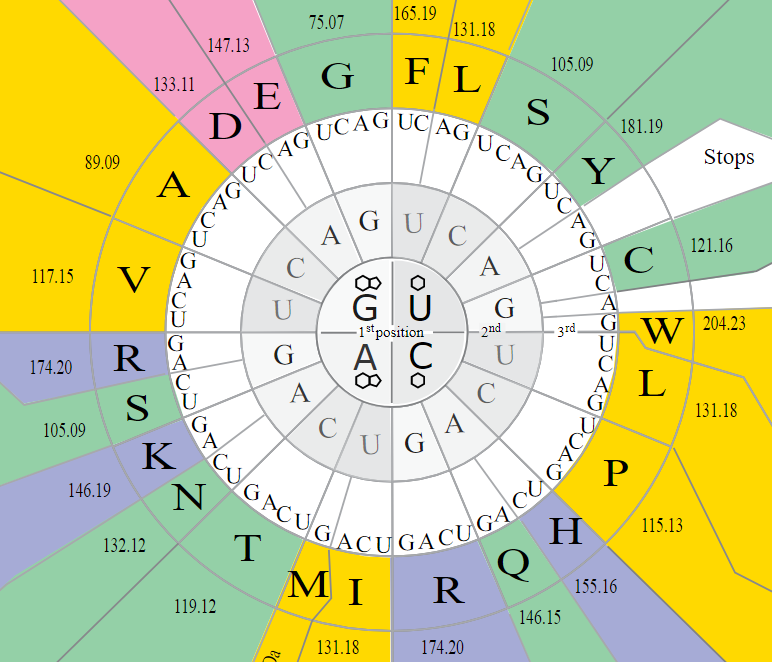
\includegraphics[width=0.6\textwidth]{imgs/Labo2/cod-gen}
\caption{Tabla de conversión ARN a aminoácido}
\label{fig:1}
\end{figure}

\subsection{Ejemplo 1}
El siguiente archivo de entrada:
\begin{lstlisting}[backgroundcolor=\color{verdito}]
UAACCUUCUACUACGUAG
\end{lstlisting}
Produce el siguiente archivo de salida:
\begin{lstlisting}[backgroundcolor=\color{verdito}]
PSTT
\end{lstlisting}

\subsection{Ejemplo 2}
El siguiente archivo de entrada:
\begin{lstlisting}[backgroundcolor=\color{verdito}]
UAACCUUCUACUACGUAG
UAGUCUCCUACGACUUUA
UAACCUUCUACUACGUAG
UAGUCUCCUACGACUUUA
\end{lstlisting}
Produce el siguiente archivo de salida:
\begin{lstlisting}[backgroundcolor=\color{verdito}]
TTPS
SPTT
TTPS
SPTT
\end{lstlisting}

\subsection{Detalles}
Cree al menos dos clases \texttt{Translator} y \texttt{FileUtil}. Los métodos mínimos para ambas clases se muestran en las tablas \ref{T1} y \ref{T2}. Además desarrolle la función \texttt{main} en un archivo aparte.


\begin{table}[H]
\begin{center}
    \begin{tabular}{ |c|c|c|c| }
    	\hline
    	\cellcolor{cl} \textbf{Tipo de retorno} & \cellcolor{cl} \textbf{Nombre del método} & \cellcolor{cl} \textbf{Argumentos} & \cellcolor{cl} \textbf{Detalle}\\ \hline \hline
         & Translator &   & Método constructor\\  \hline
         & $\sim$Translator & & Método destructor\\ \hline
         string & translate & string s & Método que traduce 1 string s\\ & & & en otro string usando las\\ & & & reglas del código genético\\ \hline
         string* & translate & string* s, int n & Método que traduce n strings\\ & & & s en otros usando las reglas\\ & & &  del código genético\\ \hline
    \end{tabular}
\end{center}
\label{T1}
\caption{Métodos de la clase \texttt{Translator}}
\end{table}


\begin{table}[H]
\begin{center}
    \begin{tabular}{ |>{\centering\arraybackslash}m{3.5cm}|>{\centering\arraybackslash}m{3.9cm}|>{\centering\arraybackslash}m{3cm}|>{\centering\arraybackslash}m{5cm}| }
    	\hline
    	\cellcolor{cl} \textbf{Tipo de retorno} & \cellcolor{cl} \textbf{Nombre del método} & \cellcolor{cl} \textbf{Argumentos} & \cellcolor{cl} \textbf{Detalle}\\ \hline \hline
         & FileUtil & string s, io\_base::openmode p & Método constructor, usa el archivo indicado por la ruta s\\ \hline
         & $\sim$FileUtil  & & Método destructor\\ \hline
         string & read & & Método que lee una línea del
\\ & & & archivo asociado al objeto\\ \hline
         string* & readLines & & Método que lee todas las líneas\\ & & & del archivo asociado al objeto\\ \hline
         int & write & string s & Método que escribe una línea
\\ & & & al archivo asociado al objeto\\ \hline
         int & write & string* s, int n & Método que escribe n líneas\\ & & & al archivo asociado al objeto\\ \hline
    \end{tabular}
\end{center}
\label{T2}
\caption{Métodos de la clase \texttt{FileUtil}}
\end{table}

Haga una corrida de prueba y genere archivos de ejemplo con entradas predefinidas para verificar la efectividad de su código.

\begin{itemize}
\item Recuerde que la idea de este laboratorio es familiarizarse con el uso de memoria dinámica, arreglos, funciones, orientación a objetos y en general la sintaxis de C++.
\item Recuerde también que por cada \texttt{new} que utilice, necesita un \texttt{delete}, sino tendrá fugas de memoria.
\item El código genético empezará y finalizará SIEMPRE con un codón de parada
\end{itemize}

\newpage

%%%%%%%%%%%%%%%%%%%%%%%%%%%%%%%%%%%%%%%%%%%%%%%%%%%%%%%%%%%%%%%%%%%%
\section{Solución}
%%%%%%%%%%%%%%%%%%%%%%%%%%%%%%%%%%%%%%%%%%%%%%%%%%%%%%%%%%%%%%%%%%%%

\subsection{Clase \texttt{FileUtil}}
Esta es la clase que se encarga del manejo de archivos; en este caso, apertura, cierre, lectura y escritura. El archivo header (\texttt{FileUtil.h}) contiene las definiciones de los métodos y atributos. En la sección pública se colocan las definiciones de los métodos constructor, destructor, los de lectura y escritura, y dos métodos auxiliares para determinar la cantidad de líneas del archivo. En la parte privada, se declaran los atributos.


\begin{minted}[linenos,autogobble,bgcolor=bg,breaklines,fontsize=\footnotesize ]{c++}
#include <string>
#include <iostream>
using namespace std;

class FileUtil
{
  public:
  	FileUtil(string s, ios_base::openmode p);
  	~FileUtil();
  	string read();
  	string* readLines();
  	int write(string s);
  	int write(string* s, int n);
    void countNumberLines();
    int getNumberLines();
  private:
    //Numero de lineas.
    int numLines;
    //Dirección de lectura.
    string ruta;
    //Modo de lectura.
  	ios_base::openmode modo;
    //Linea leida.
    string line;
    //Puntero con la direccion del arreglo de las lineas leidas.
    string* lines;

};
\end{minted}

\subsubsection{Implementación}

\begin{itemize}
\item \textbf{Método constructor:}\\
El método constructor recibe dos argumentos, que corresponden a la ruta del archivo a procesar, y el modo de procesamiento. Este modo es una variable del tipo \texttt{ios\_base::openmode}, y en este caso existen dos posibles modos válidos: \texttt{in} y \texttt{out}. Estos argumentos se asignan a los atributos ``ruta'' y ``modo'', respectivamente. Además en el constructor se inicializan los atributos ``lines'' y ``numLines''.


\begin{minted}[linenos,autogobble,bgcolor=bg,breaklines,fontsize=\footnotesize ]{c++}
FileUtil::FileUtil (string s, ios_base::openmode p)
{
  this->ruta = s;
  this->modo = p;
  this->numLines = 0;
  int n = FileUtil::getNumberLines();
  this->lines = new string[n];
}

};
\end{minted}

\item \textbf{Método destructor:}\\
En el método destructor se hace la liberación de memoria correspondiente al atributo de tipo arreglo de tamaño variable, ``lines''.
\begin{minted}[linenos,autogobble,bgcolor=bg,breaklines,fontsize=\footnotesize ]{c++}
FileUtil::~FileUtil()
{
  delete [] this->lines;
}
\end{minted}


\item \textbf{Método \texttt{read()}:}\\

Este método usa la biblioteca \texttt{fstream} para crear un objeto llamado ``myFile'', sobre el cual se ejecutan las operaciones. En este caso, se lee una única línea, y el contenido de ésta se asigna al atributo ``line'', de tipo string, que es el valor de retorno y que luego se pasará a los métodos de traducción. En este caso, se asigna directamente el valor a ``numLines'' = 1. 

\begin{minted}[linenos,autogobble,bgcolor=bg,breaklines,fontsize=\footnotesize ]{c++}
string FileUtil::read(){
  fstream myFile(this->ruta.c_str(),this->modo);
  if (myFile.is_open())
 {
    getline(myFile,this->line);
    this->numLines = 1;
    myFile.close();
  }
  return this->line;
}
\end{minted}

\item \textbf{Método \texttt{readLines()}:}\\

Este método permite leer un archivo que posee múltiples líneas de texto. Se usa una variable auxiliar ``count'' para recorrer las líneas. En cada línea leída, su contenido se asigna al atributo ``line'', y éste se agrega al arreglo de strings llamado ``lines[]'', que es el retorno de la función. De esta manera, se tiene que este método retorna un arreglo de strings que contiene todas las líneas de texto leídas del archivo de origen. 

\begin{minted}[linenos,autogobble,bgcolor=bg,breaklines,fontsize=\footnotesize ]{c++}
string* FileUtil::readLines(){
  int count = 0;
  fstream myFile(this->ruta.c_str(),this->modo);
  if (myFile.is_open())
 {
    while (getline(myFile,this->line))
    {
      this->lines[count] = this->line;
      //cout << this->line << '\n';
      count++;
    }
    myFile.close();
  }
  return this->lines;
}
\end{minted}


\item \textbf{Métodos \texttt{write()}:}

El primer método \texttt{write()} se encarga de escribir una única línea de texto en un archivo. Su argumento es un string que contiene el texto a escribir. En este caso, el valor de retorno es 0 si el proceso se llevó a cabo exitosamente, y 1 si ocurrió algún error. 

\begin{minted}[linenos,autogobble,bgcolor=bg,breaklines,fontsize=\footnotesize ]{c++}
int FileUtil::write (string s)
{
  fstream myFile(this->ruta.c_str(),this->modo);

  if (myFile.is_open())
  {
    myFile << s;
    myFile.close();
    return 0;
  }
  else
  {
    cout << "Unable to open file";
    return 1;
  }
}
\end{minted}

El segundo método llamado \texttt{write()}, recibe como argumento un arreglo de strings \texttt{s} con el texto a escribir en un archivo, y un entero \texttt{n} que indica el total de líneas que se desea escribir. Se usa un incrementador llamado ``count'' que sirve para recorrer el arreglo y accesar su contenido, asignándoselo al stream ``myFile''.

\begin{minted}[linenos,autogobble,bgcolor=bg,breaklines,fontsize=\footnotesize ]{c++}
int FileUtil::write (string* s, int n)
{
  fstream myFile(this->ruta.c_str(),this->modo);
  if (myFile.is_open())
  {
    for (int count = 0; count < n; count++)
    {
      myFile << *(s+count);
      myFile << endl;
    }
    myFile.close();
    return 0;
  }
  else
  {
    cout << "Unable to open file";
    return 1;
  }
}
\end{minted}


\item \textbf{Métodos auxiliares:}

El método \texttt{getNumberLines()} devuelve el número de líneas de texto de un archivo. Para esto, llama al método \texttt{countNumberLines()}, el cual recorre todas las líneas del archivo, incrementando un contador llamado ``numLines'' (que es un atributo de esta clase). El valor final de numLines es el retorno de este método.

\begin{minted}[linenos,autogobble,bgcolor=bg,breaklines,fontsize=\footnotesize ]{c++}
int FileUtil::getNumberLines()
{
  FileUtil::countNumberLines();
  return this->numLines;
}
\end{minted}


\begin{minted}[linenos,autogobble,bgcolor=bg,breaklines,fontsize=\footnotesize ]{c++}
void FileUtil::countNumberLines()
{
  this->numLines = 0;
  fstream myFile(this->ruta.c_str(),this->modo);
  if (myFile.is_open())
 {
    while (getline(myFile,this->line))
    {
      this->numLines++;
    }
    myFile.close();
  }
}

\end{minted}

\end{itemize}
\subsection{Clase \texttt{Translator}}

Esta clase es la que contiene los métodos encargados de la traducción de los codones. En el header (\texttt{Translator.h}) se definen los métodos y atributos.
\begin{minted}[linenos,breaklines,bgcolor=bg,fontsize=\footnotesize ]{c++}
#include <string>
#include <iostream>
using namespace std;

class Translator {
	public:
    	Translator();
    	~Translator();
    	string translate (string s);
    	string* translate (string* s, int n);
    	string asociar(int i, int j);
    	string error();
    private:
};
\end{minted}

\subsubsection{Implementación}

\begin{itemize}

\item \textbf{Método \texttt{translate(string s)}:}

Es el método principal de la clase (y de todo el programa), ya que es el que realiza toda la comparación necesaria para la traducción. Se le pasa como argumento un string que corresponde a una línea de texto, previamente obtenida de un archivo \texttt{.txt}.

Las primeras operaciones que se realizan son de conteo de cantidad de caracteres y cantidad de tríos de letras (codones) en la línea de texto.

\begin{minted}[linenos,breaklines,bgcolor=bg,fontsize=\footnotesize ]{c++}
string Translator::translate (string s) {
  string codones = s; // Codones leidos de una fila del archivo .txt
  int tamano = codones.size(); // Cantidad de letras en la fila  
  int cantidadTrios = tamano / 3; // Cantidad de grupos de tres letras
\end{minted}
Se crea el arreglo llamado ``arregloTrios'', en el cual, cada elemento será un codón. Como este arreglo es de tamaño variable, se utiliza memoria dinámica.

\begin{minted}[linenos,breaklines,bgcolor=bg,fontsize=\footnotesize ]{c++}
  string* arregloTrios;
  arregloTrios = new string[cantidadTrios];
\end{minted}

Igualmente se crea el arreglo ``traducido'', el cual va a contener las letras correspondientes a los aminoácidos, una vez terminada la traducción.

\begin{minted}[linenos,breaklines,bgcolor=bg,fontsize=\footnotesize ]{c++}
  string* traducido;
  traducido = new string[cantidadTrios-2];
\end{minted}

Posteriormente, se incluyen las rutinas de verificación de condiciones necesarias. La primera, es que la cantidad de letras en el string de origen sea múltiplo de 3; para esto, se incluye todo el código posterior dentro de un \texttt{if}. 

\begin{minted}[linenos,breaklines,bgcolor=bg,fontsize=\footnotesize ]{c++}
	if (tamano % 3 == 0 ){ 
		...
	} else {
		error();
		cout << "Error: cantidad de caracteres no es multiplo de 3." << endl;
  	}
\end{minted}

El siguiente bloque asigna a cada elemento de arregloTrios un conjunto de 3 letras del string original:

\begin{minted}[linenos,breaklines,bgcolor=bg,fontsize=\footnotesize ]{c++}
	int i = 0;
	int c = 0;
	for (int x = 0; x < cantidadTrios; x++ ){
		arregloTrios[i] = codones.substr(c, 3); // La funcion substr(a,b) guarda b letras de la string desde la posicion a
		i++;
		c += 3;
   		 }
\end{minted}

Luego, habiendo definido previamente los codones de parada válidos:

\begin{minted}[linenos,breaklines,bgcolor=bg,fontsize=\footnotesize ]{c++}
  string cdnparada1 = "UGA";
  string cdnparada2 = "UAG";
  string cdnparada3 = "UAA";
\end{minted}

Se procede a verificar que la línea de texto evaluada comience y termine con un codón de parada válido:

\begin{minted}[linenos,breaklines,bgcolor=bg,fontsize=\footnotesize ]{c++}
    if ( !(arregloTrios[0] == cdnparada1 || arregloTrios[0] == cdnparada2 || arregloTrios[0] == cdnparada3 ) ){ //Compara el trio del inicio
		error();
    cout << "Error: la hilera no tiene codones de parada validos." << endl;
		
	} else if (!(arregloTrios[cantidadTrios-1] == cdnparada1 || arregloTrios[cantidadTrios-1] == cdnparada2 || arregloTrios[cantidadTrios-1] == cdnparada3)){ //Compara el trio del final
		error();
    cout << "Error: la hilera no tiene codones de parada validos." << endl;
		
	} else { //trios de parada existen
		cout << "La hilera tiene codones de parada validos." << endl;
\end{minted}
La siguiente condición consiste en verificar que todos los caracteres contenidos en el texto sean válidos, es decir, ``A'', ``U'', ``G'' o ``C''.

\begin{minted}[linenos,breaklines,bgcolor=bg,fontsize=\footnotesize ]{c++}
		for (int d = 0; d < tamano; d++){
			letras [d] = codones.substr(d,1); //guarda las letras una por una como string
		}

		for (int t=0;t<tamano;t++){
  		// cout << letras[t] <<endl;
  		if (letras[t] == "A" || letras[t] == "C" || letras[t] == "G" || letras[t] == "U"  ) {
  			cout << letras [t] << ": Todo bien, letra valida." << endl;
  			} else {
  			error();
        cout << letras[t] << ": Error: letra no valida." << endl;
  			}
  		}  
\end{minted}

Habiéndose cumplido todas las condiciones, se procede luego con la traducción. En esta sección se empieza creando un \texttt{string} en donde se va a almacenar las letras de la traducción. Con un \texttt{for()} que ignora los tríos del principio y el final (ya se verificó que son codones de parada válidos, por lo que no se traducen) se compara cada codón del string que se quiere traducir \texttt{arregloTrios[]} con los codones de que conforman las posibles combinaciones de letras de las bases nitrogenadas. Cuando uno de estos tríos coincida se llama al método \texttt{asociar()} al que se le envían como argumentos la posición del codón que coincidió para que así asocie a cuál aminoácido corresponde. Lo que retorna la función \texttt{asociar()} se almacena en el \texttt{string} creado anteriormente, al que se le van agregando los resultados utilizando la función \texttt{append()} de las bibliotecas de C++.

\begin{minted}[linenos,breaklines,bgcolor=bg,fontsize=\footnotesize ]{c++}
string traducido;
  	for (int r = 1; r < cantidadTrios-1; r++ ){ //Ignorando el primer y ultimo trios porque ya se comprobó que son de parada
  		for (int p = 0; p < 64; p++){
  			if ( arregloTrios[r] == cdntraduccion[p] ) {
  				string letra = asociar(p, r-1);
  				traducido.append(letra);
  			}
  		}
  	}
\end{minted}


\item \textbf{Método \texttt{translate(string* s, int n)}:}

Es el método encargado de la traducción de un archivo con varias líneas de codones. Recibe como argumento un puntero \texttt{string *s} con dirección del primer elemento de un arreglo de \texttt{string}s donde se guardan las cadenas que se van a traducir. También se le envía un entero \texttt{n} que le indica al método la cantidad de elementos que posee el arreglo, es decir, la cantidad de líneas que se quieren traducir.

\begin{minted}[linenos,breaklines,bgcolor=bg,fontsize=\footnotesize ]{c++}
string* Translator::translate (string* s, int n){
  string* traduccion = new string [n];
\end{minted}
Cuando se obtienen los parámetros se reserva memoria dinámica (utilizando \texttt{new}) para un nuevo puntero que almacena la dirección de la traducción realizada,este puntero tiene una dimensión \texttt{n}, como se observa en la línea 2.

\begin{minted}[linenos,breaklines,bgcolor=bg,fontsize=\footnotesize ]{c++}
  for (int q = 0; q < n; q++ ){
    traduccion[q] = translate(s[q]);
  }
\end{minted}
Luego se procede a llamar al método \texttt{translate()} varias veces mediante un ciclo \texttt{for()}, \texttt{n} veces. En donde se le envían cada una de las líneas que se quieren traducir, y lo que retorna este método se almacena en la variable creada anteriormente.

\begin{minted}[linenos,breaklines,bgcolor=bg,fontsize=\footnotesize ]{c++}
  return traduccion;
\end{minted}

Finalmente se procede a devolver el puntero que apunta al arreglo que almacena las traducciones.

\item \textbf{Método \texttt{asociar()}:}

Método auxiliar utilizado para asociar directamente un codón (un elemento del arreglo arregloTrios[ ] con su correspondiente letra (aminoácido). Recibe la posición con la que coincidió el trío de codones, y la compara mediante un \texttt{switch()} para saber a cuál aminoácido corresponde. Cada uno de los 64 casos corresponde a un aminoácido representado por la una única letra. La función regresa esta letra en forma de \texttt{string}.

\begin{minted}[linenos,breaklines,bgcolor=bg,fontsize=\footnotesize ]{c++}
string Translator::asociar (int i, int j){
    string letra;
    switch(i){
      case 0:
        letra = "G";
  		break;
      case 1:
        letra = "G";
  		break;
      ...
      ...
      ...
      case 63:
        letra = "F";
  		break;
      }
    return letra;
}
\end{minted}


\item \textbf{Método \texttt{error()}:}

Se incluyó un método para mostrar un mensaje de error cuando se presente alguna situación indeseada en la ejecución del programa.

\begin{minted}[linenos,breaklines,bgcolor=bg,fontsize=\footnotesize ]{c++}
void Translator::error(){
  cout << "|||||||| ERROR EN LA EJECUCION DEL PROGRAMA ||||||||" << endl;
}
\end{minted}
\end{itemize}


\section{Resultados}

Una vez que se tienen todos los códigos listos y en sus respectivas carpetas, se compila con un \texttt{makefile} y se ejecuta. El programa solicita mediante la terminal que se ingrese la ruta donde se ubica el archivo \texttt{.txt} con las cadenas a traducir, y posteriormente nos solicita la ruta del archivo en donde se va a escribir la traducción. Si no se encuentra ningún problema, se crea correctamente el archivo de salida. Este archivo se puede leer con cualquier editor de texto, en la Figura \ref{fig:trans1} se muestra a la izquierda el archivo que contiene la cadena a traducir. Y a la derecha se puede observar el archivo en donde se escribió la traducción del mismo. En este caso corresponde a únicamente una línea de 4 letras. 

\begin{figure}[htbp]
\centering
\subfigure[Cadena de codones.]{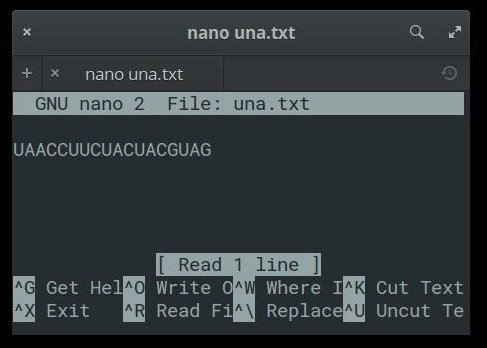
\includegraphics[width=54mm]{imgs/Labo2/INuna.jpeg}}
\subfigure[Traducción de la cadena.]{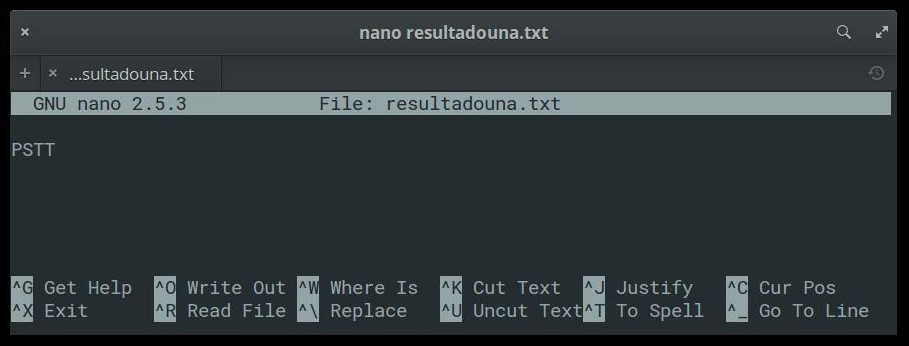
\includegraphics[width=101.5mm]{imgs/Labo2/OUTuna.jpeg}}
\caption{Traducción de una única línea.} \label{fig:trans1}
\end{figure}

Cuando al programa se le indica una ruta de un archivo con varias líneas como el que se observa en la imagen izquierda de la Figura \ref{fig:trans2}, este se ejecuta de igual manera, y escribe un archivo con la traducción correspondiente como se observa en la imagen de la derecha.

\begin{figure}[htbp]
\centering
\subfigure[Varias cadenas de codones.]{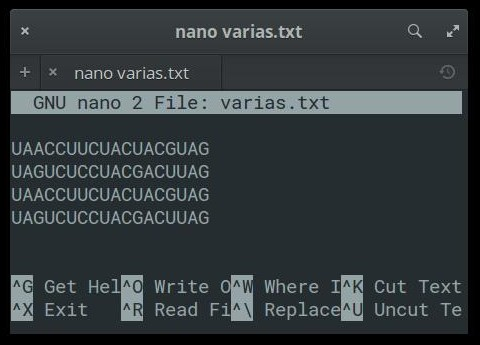
\includegraphics[width=54mm]{imgs/Labo2/INvarias.jpeg}}
\subfigure[Traducción de las cadenas.]{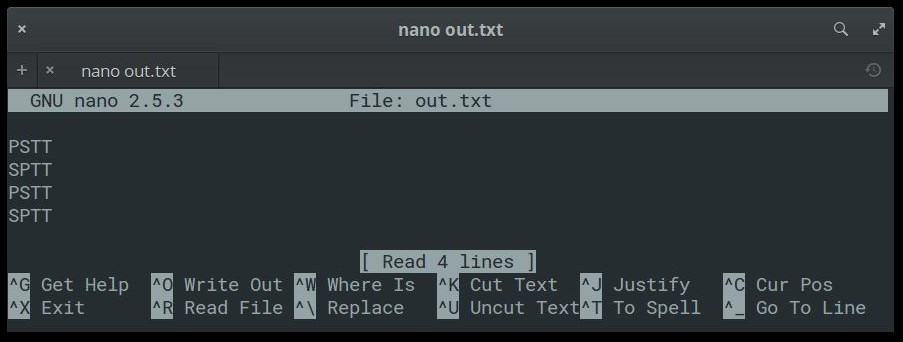
\includegraphics[width=102mm]{imgs/Labo2/OUTvarias.jpeg}}
\caption{Traducción de varias cadenas de codones.} \label{fig:trans2}
\end{figure}

\section{Conclusiones}
El objetivo principal del laboratorio se cumplió satisfactoriamente. Se logró familiarizarse con los comandos de C++ y el paradigma de programación orientada a objetos. También es importante notar el uso del concepto de reserva de memoria dinámica, así como su debida liberación después de su uso. Además se practicó la correcta documentación del código utilizando \texttt{Doxygen}, y la compilación mediante un \texttt{makefile}. 


%%%%%%%%%%%%%%%%%%
%--> LABORATORIO 3
%%%%%%%%%%%%%%%%%%
%%%%%%%%%%%%%%%%%%%%%%%%%%%%%%%%%%%%%%%%%%%%%%%%%%%%%%%%%%%%%%%%%%%%%%%%%%%%%%%%%%%%%%%%%%%%%%%%%%%%
\newpage
\section{Introducción}
%%%%%%%%%%%%%%%%%%%%%%%%%%%%%%%%%%%%%%%%%%%%%%%%%%%%%%%%%%%%%%%%%%%%%%%%%%%%%%%%%%%%%%%%%%%%%%%%%%%

Se define herencia como el proceso mediante el cual una clase adquiere las propiedades (atributos) y comportamientos (métodos) de otra clase. 

En programación orientada a objetos comprender los conceptos de herencia, polimorfismo, funciones virtuales y sobrecarga es de vital importancia para lograr aplicar el concepto de clases a la resolución de diferentes tipos de problemas en las que usar estos conceptos nos ayuda a modelar la solución de una manera más eficiente y adecuada. 

%%%%%%%%%%%%%%%%%%%%%%%%%%%%%%%%%%%%%%%%%%%%%%%%%%%%%%%%%%%%%%%%%%%%%%%%%%%%%%%%%%%%%%%%%%%%%%%%%%%
\subsection{Objetivos}
\begin{enumerate}
\item Repasar y utilizar los conceptos de herencia, polimorfismo y sobrecarga. 
\item Practicar la sobrecarga de operadores para simplificar algunas operaciones.
\item Realizar un diagrama UML que permita visualizar la relación entre clases. 
\end{enumerate}
%%%%%%%%%%%%%%%%%%%%%%%%%%%%%%%%%%%%%%%%%%%%%%%%%%%%%%%%%%%%%%%%%%%%%%%%%%%%%%%%%%%%%%%%%%%%%%%%%%%
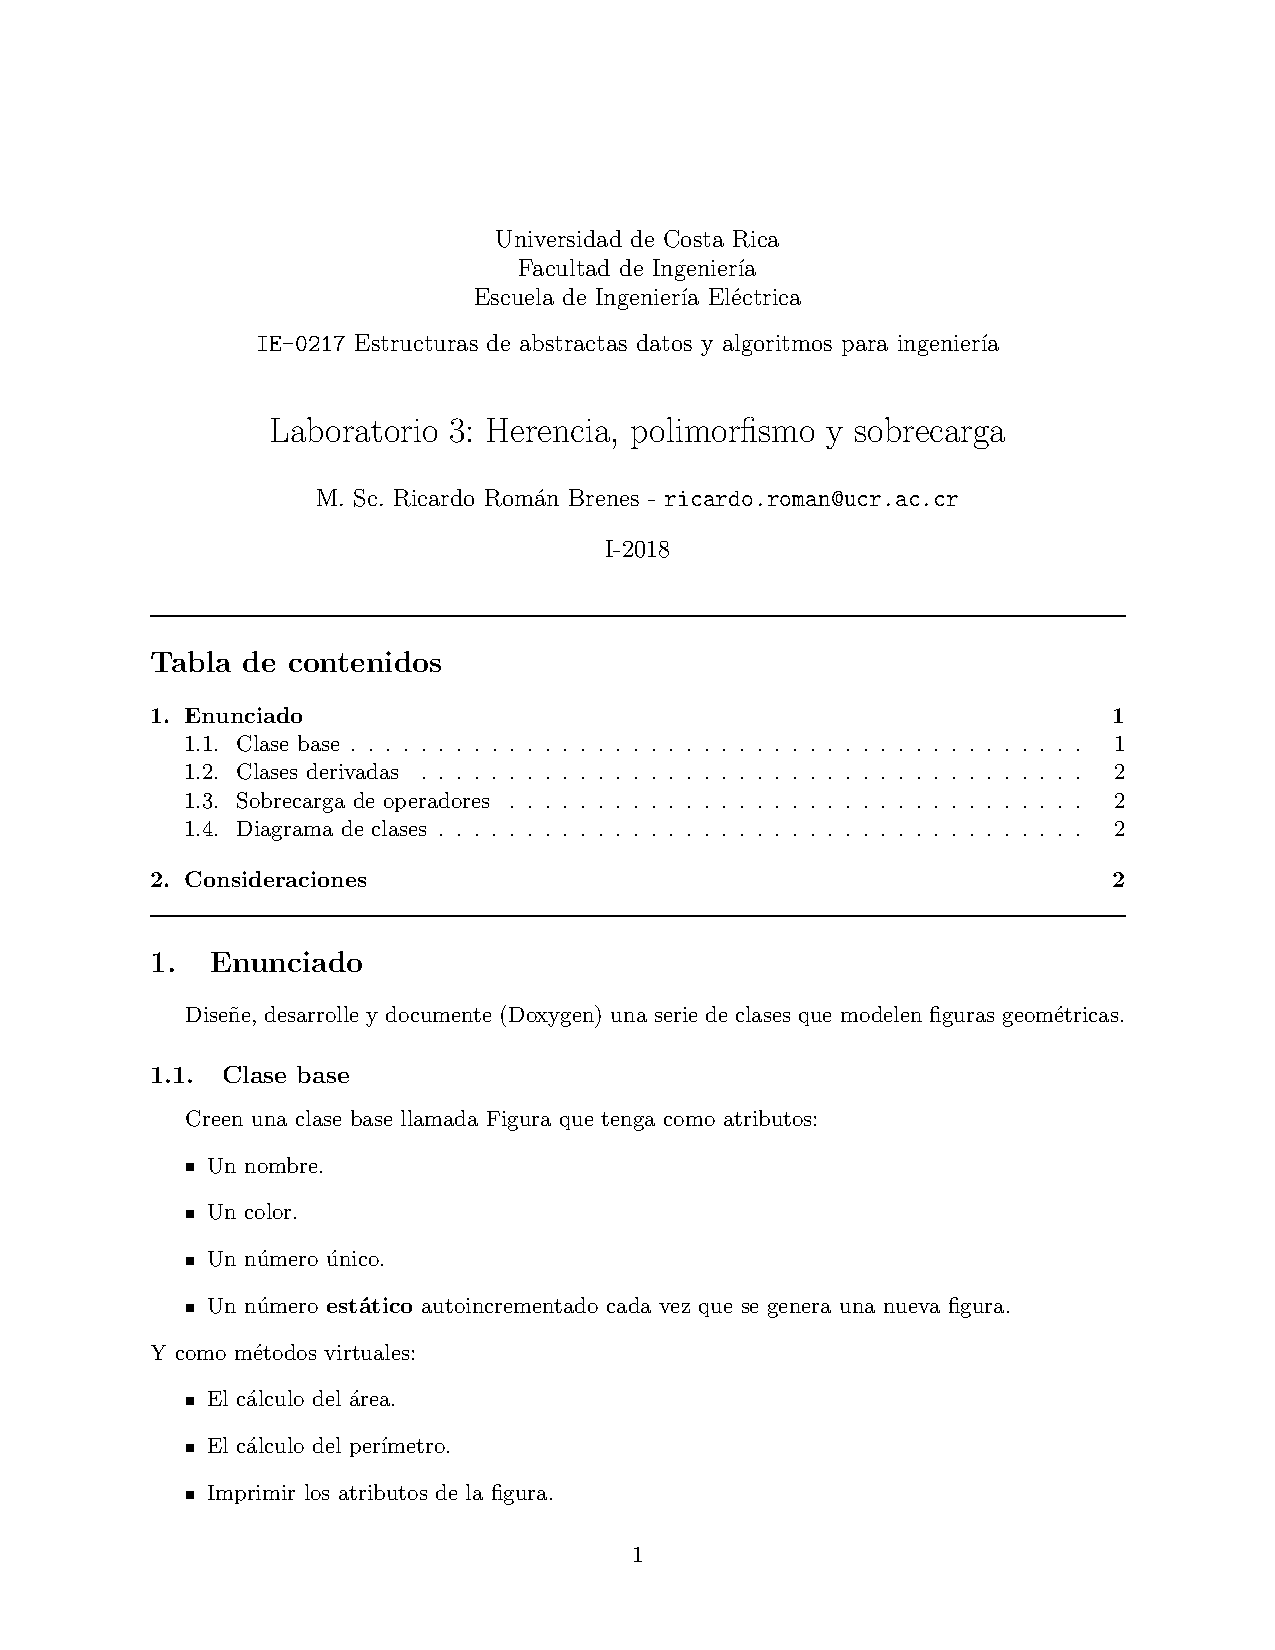
\includepdf[pages=1,pagecommand=\section{Enunciado}]{enunciados/enun3}
\includepdf[pages=2,pagecommand={}]{enunciados/enun3}
%%%%%%%%%%%%%%%%%%%%%%%%%%%%%%%%%%%%%%%%%%%%%%%%%%%%%%%%%%%%%%%%%%%%%%%%%%%%%%%%%%%%%%%%%%%%%%%%%%%

%%%%%%%%%%%%%%%%%%%%%%%%%%%%%%%%%%%%%%%%%%%%%%%%%%%%%%%%%%%%%%%%%%%%%%%%%%%%%%%%%%%%%%%%%%%%%%%%%%%
\section{Solución}
%\begin{minted}[linenos,autogobble,bgcolor=bg,breaklines,fontsize=\footnotesize ]{c++}

%\end{minted}
%%%%%%%%%%%%%%%%%%%%%%%%%%%%%%%%%%%%%%%%%%%%%%%%%%%%%%%%%%%%%%%%%%%%%%%%%%%%%%%%%%%%%%%%%%%%%%%%%%%
\subsection{Clase base: \texttt{Figure()}}
La clase \texttt{Figure()} es la clase base del programa, de donde las demás clases heredan. En el \textit{header} \texttt{Figure.h} se definen los métodos y atributos de la clase. En la sección pública se colocan las definiciones de los métodos constructor, destructor, así como los métodos virtuales para calcular el área, el perímetro, y la función encargada de imprimir los datos de la clase. Se declaran los atributos como protegidos, en estos se incluye el nombre, el color, un número único para el objeto, y un número estático que se incrementa cada vez que se genera una figura, para esto se implementa un método más.

\begin{minted}[linenos,autogobble,bgcolor=bg,breaklines,fontsize=\footnotesize ]{c++}
#include <string>
#include <iostream>
using namespace std;
#ifndef FIGURE_H
#define FIGURE_H

///@class Figure
class Figure {
  public:
    Figure();
    ~Figure();
    virtual double area() = 0 ; 
    virtual double perimetro() = 0; 
    virtual void imprimir() = 0;
  protected:
    int getNumAutoInc();
    string nombre;
    string color;
    int numUnico;
    static int numAutoInc; 
  private:
};
#endif
\end{minted}

\subsection{Clase derivada: \texttt{Rectangle()}}

La clase \texttt{Rectangle()} hereda de la clase base; como se observa a la hora de declararlo mediante la línea \texttt{class Rectangle : public Figure}. En el archivo \texttt{Rectangle.h} se observan los métodos que contiene esta clase. Para los cálculos respectivos a un rectángulo, se declaran dos variables protegidas de tipo \texttt{double} para almacenar el largo y el ancho de la figura.
\begin{minted}[linenos,autogobble,bgcolor=bg,breaklines,fontsize=\footnotesize ]{c++}
#include <string>
#include <iostream>
#include "../include/Figure.h"
using namespace std;
#ifndef RECTANGLE_H
#define RECTANGLE_H

///@class Rectangle
class Rectangle : public Figure {
  public:
    Rectangle();
    Rectangle(string nombre, string color, int numUnico, double largo, double ancho);
    Rectangle(const Rectangle& r);
    ~Rectangle();
    double area();
    double perimetro();
    void imprimir();
    void operator~();
    void operator!();
    void operator=(const Rectangle& r);
  protected:
    double largo;
    double ancho;
  private:
};
#endif
\end{minted}

\subsubsection{Métodos de \texttt{Rectangle()}}
\begin{itemize}
\item \textbf{Constructor vacío:}

	Cuando se crea un objeto de tipo \texttt{Rectangle} sin pasarle ningún argumento, se utiliza este constructor. Aquí se le solicita al usuario que ingrese los datos necesarios para crear el objeto con sus atributos bien definidos. Se solicita el nombre, el color, el número único y las medidas de los lado, todo lo anterior se guarda en las variables de los atributos respectivos utilizando el operador \texttt{this->}.
    \begin{minted}[linenos,autogobble,bgcolor=bg,breaklines,fontsize=\footnotesize ]{c++}
Rectangle::Rectangle(){
  cout << endl <<"Ingrese el nombre del rectangulo:  ";
  cin >> this->nombre;
  cout << endl << "Ingrese el color del rectangulo:  ";
  cin >> this->color;
  cout << endl << "Ingrese un numero unico para identificar el rectangulo:  ";
  cin >> this->numUnico;
  cout << endl << "Ingrese la medidad del lado largo del rectangulo:  ";
  cin >> this->largo;
  cout << endl << "Ingrese la medidad del ancho del rectangulo:  ";
  cin >> this->ancho;
}   
    \end{minted}
    
\item \textbf{Constructor con parámetros:}

	El constructor con parámetros se utiliza cuando se crea un objeto y se le pasan los atributos como argumentos al método.
	\begin{minted}[linenos,autogobble,bgcolor=bg,breaklines,fontsize=\footnotesize ]{c++}
Rectangle::Rectangle(string nombre, string color, int numUnico, double largo, double ancho) {
  this->nombre = nombre;
  this->color = color;
  this->numUnico = numUnico;
  this->largo = largo;
  this->ancho = ancho;
}
   \end{minted}

\item \textbf{Constructor por copia:}

Para crear un objeto inicializándolo con otro ya existente. Se pasa una referencia al objeto existente, y se copian sus atributos en el nuevo objeto.

\begin{minted}[linenos,autogobble,bgcolor=bg,breaklines,fontsize=\footnotesize ]{c++}
Rectangle::Rectangle(const Rectangle &copyRectangle){
  this->nombre    = copyRectangle.nombre;
  this->color     = copyRectangle.color;
  this->numUnico  = copyRectangle.numUnico;
  this->largo     = copyRectangle.largo;
  this->ancho     = copyRectangle.ancho;
}
\end{minted}

\item \textbf{Área y perímetro:}

	Los dos métodos para calcular el área y el perímetro simplemente en el \texttt{return} realizan la operación necesaria para obtener el resultado. Para obtener las medidas de los lados se utilizan los atributos utilizando el puntero \texttt{this->}. Por el tipo de cálculo a realizar, las funciones devuelven el resultado tipo \texttt{double}.
    
	\begin{minted}[linenos,autogobble,bgcolor=bg,breaklines,fontsize=\footnotesize ]{c++}
double Rectangle::area(){
  return (this->largo*this->ancho);
}
\end{minted}

	\begin{minted}[linenos,autogobble,bgcolor=bg,breaklines,fontsize=\footnotesize ]{c++}
double Rectangle::perimetro(){
  return ((2*(this->largo))+(2*(this->ancho)));
}
\end{minted}

\item \textbf{Método imprimir:}

	Imprime todos los datos del objeto.
    	\begin{minted}[linenos,autogobble,bgcolor=bg,breaklines,fontsize=\footnotesize ]{c++}
void Rectangle::imprimir() {
  cout << "Nombre: " << this->nombre << endl;
  cout << "Color: " << this->color << endl;
  cout << "Número Único: " << this->numUnico << endl;
  cout << "Largo: " << this->largo << endl;
  cout << "Ancho: " << this->ancho << endl;
  cout << "Número Autoincrementado: " << this->numAutoInc << endl;
}
\end{minted}

\item \textbf{Sobrecarga de operadores}\\
Se implementa la sobrecarga de los operadores \texttt{!, \~} y \texttt{=}. El operador \texttt{!} se utiliza para calcular el área y el perímetro; \texttt{\~} se utiliza para imprimir los datos del objeto, y el operador \texttt{=} se utiliza para igualar o copiar un objeto en otro.

\begin{minted}[linenos,autogobble,bgcolor=bg,breaklines,fontsize=\footnotesize ]{c++}
void Rectangle::operator~(){
  imprimir();
}
void Rectangle::operator!(){
  cout << "Area: " << area() << endl;
  cout << "Perimetro: " << perimetro() << endl;
}
void Rectangle::operator=(const Rectangle& r)
{
  this->nombre    = r.nombre;
  this->color     = r.color;
  this->numUnico  = r.numUnico;
  this->largo     = r.largo;
  this->ancho     = r.ancho;
}
\end{minted}


\end{itemize}



\subsection{Clase derivada: \texttt{Triangle()}}

\begin{minted}[linenos,autogobble,bgcolor=bg,breaklines,fontsize=\footnotesize ]{c++}
#include <string>
#include <iostream>
#include "../include/Figure.h"
#ifndef TRIANGLE_H
#define TRIANGLE_H

class Triangle : public Figure
{
  public:
    Triangle();
    Triangle(string n, string c, int num, double l1, double l2, double l3);
    Triangle(const Triangle& r);
    ~Triangle();
    double area();
    double perimetro();
    void imprimir();
    void operator~();
    void operator!();
    void operator=(const Triangle& t);
  private:
	  double lado1;
	  double lado2;
	  double lado3;
	  string tipo;	//tipo de triangulo
	  void initIDs();	//para pedir valores de atributos al usuario
  	void initLados(); //para pedir valores de los lados al usuario
  	bool desigualdad(double a, double b, double c); //teorema de la desigualdad para ver si con lados ingresados se puede formar un triangulo
  	bool verifLados(double l1, double l2, double l3);
  	void verifTipo(double l1, double l2, double l3);
  };

#endif

\end{minted}

\subsubsection{Métodos de \texttt{Triangle()}}

\begin{itemize}
\item \textbf{Constructor vacío:}\\
Si se crea una instancia de \texttt{Triangle} utilizando el constructor vacío, se llamará a los métodos que se encargan de inicializar los atributos correspondientes. De esta manera, no se permite que existan objetos sin alguno de los atributos asignado.
\begin{minted}[linenos,autogobble,bgcolor=bg,breaklines,fontsize=\footnotesize ]{c++}
Triangle::Triangle(){
	initIDs();
	initLados();
	verifTipo(this->lado1,this->lado2,this->lado3);
}
\end{minted}

\item \textbf{Constructor con parámetros:}\\
Se puede crear un objeto \texttt{Triangle} pasándole los atributos en el constructor, en un orden específico. En este caso, se debe llamar a un método que verifica si los lados con los que se desea construir este objeto son válidos (más adelante se explica de qué se trata esto).
\begin{minted}[linenos,autogobble,bgcolor=bg,breaklines,fontsize=\footnotesize ]{c++}
Triangle::Triangle(string n, string c, int num, double l1, double l2, double l3){
	if (verifLados(l1,l2,l3) == false){
		initLados();
	}
	else {
		this->lado1 = l1;
		this->lado2 = l2;
		this->lado3 = l3;
	}
	this->nombre = n;
	this->color = c;
	this->numUnico = num;
	verifTipo(this->lado1,this->lado2,this->lado3);
}
\end{minted}

\item \textbf{Constructor por copia:}\\
Para crear un objeto inicializándolo con otro ya existente. Se pasa una referencia al objeto existente. 

\begin{minted}[linenos,autogobble,bgcolor=bg,breaklines,fontsize=\footnotesize ]{c++}
Triangle::Triangle(const Triangle &copy){
  this->nombre    = copy.nombre;
  this->color     = copy.color;
  this->numUnico  = copy.numUnico;
  this->lado1     = copy.lado1;
  this->lado2     = copy.lado2;
  this->lado3     = copy.lado3;
  this->tipo      = copy.tipo;
}
\end{minted}


\item \textbf{Inicializador de identificadores (\texttt{initIDs()})}\\
Así se denominó al método que solicita al usuario los valores de los atributos \texttt{nombre}, \texttt{color} y \texttt{numUnico}, para asignárselos al objeto creado. No se hace verificación de tipos. 

\begin{minted}[linenos,autogobble,bgcolor=bg,breaklines,fontsize=\footnotesize ]{c++}
void Triangle::initIDs(){
	string n, c;
	int num;
	cout << endl << "Ingrese el nombre del triangulo:  ";
	cin >> n;
	cout << endl << "Ingrese el color del triangulo:  ";
	cin >> c;
	cout << endl << "Ingrese un numero unico para identificar el triangulo: ";
	cin >> num;
	this->nombre = n;
	this->color = c;
	this->numUnico = num;
}
\end{minted}

\item \textbf{Método \texttt{initLados()}}\\
Solicita al usuario los valores de los lados, de tipo \texttt{double}. Antes de asignarle estos valores al objeto creado, utiliza el método \texttt{verifLados()} para determinar si son valores válidos. El ciclo \texttt{do ... while} permite ejecutar la solicitud al usuario, y luego verificar si se cumple la condición; de no ser así, la solicitud se vuelve a realizar.

\begin{minted}[linenos,autogobble,bgcolor=bg,breaklines,fontsize=\footnotesize ]{c++}
void Triangle::initLados(){
	double l1, l2, l3;
	do {
		cout << endl <<"Ingrese el primer lado: ";
		cin >> l1;
		cout << endl << "Ingrese el segundo lado:  ";
		cin >> l2;
		cout << endl << "Ingrese el tercer lado:  ";
		cin >> l3;
	} while (verifLados(l1,l2,l3)==false);
	this->lado1 = l1;
	this->lado2 = l2;
	this->lado3 = l3;
}
\end{minted}

\item \textbf{Método \texttt{verifLados()}}\\
Este método verifica si los valores que se quiere asignar a los lados del triángulo creado, son valores válidos; esto es, si cumplen el teorema de la desigualdad triangular. Este teorema establece que los lados l1, l2 y l3 forman un triángulo si la suma de cualesquiera dos de ellos es mayor al lado restante. Este teorema se implementa aquí con otro método llamado \texttt{desigualdad()}, que retorna un valor booleano. Se indica en un mensaje si los lados ingresados son válidos.

\begin{minted}[linenos,autogobble,bgcolor=bg,breaklines,fontsize=\footnotesize ]{c++}
bool Triangle::verifLados(double l1, double l2, double l3){
	if (desigualdad(l1,l2,l3) == true){
		cout << endl << "Lados válidos" << endl << endl;
		return true;
	}
	else{
		cout << endl<< "Los lados ingresados (" << l1 << "," << l2 << "," << l3 << ") no pueden formar un triángulo. Ingrese lados válidos." << endl;
		return false;
	}
}

bool Triangle::desigualdad(double a, double b, double c){
	if ((a<b+c) && (b<a+c) && (c<a+b)){
		return true;
	}
	else {
		return false;
	}
}
\end{minted}

\item \textbf{Método \texttt{verifTipo()}}\\
Evalúa los lados del triángulo para determinar si este es ``equilátero'', ``isósceles'' o ``escaleno'', y asigna el valor resultante al atributo \texttt{tipo}.

\begin{minted}[linenos,autogobble,bgcolor=bg,breaklines,fontsize=\footnotesize ]{c++}
void Triangle::verifTipo(double l1, double l2, double l3){
	if (l1 == l2 && l2 == l3){
		this->tipo="equilatero";
	}
	else if ((l1==l2)||(l1==l3)||(l2==l3)){
		this->tipo="isosceles";
	}
	else {
		this->tipo="escaleno";
	}
}
\end{minted}

\item \textbf{Métodos \texttt{perimetro()} y \texttt{area()}}\\
El método \texttt{perimetro()} devuelve la suma de los lados, mientras que \texttt{area()} calcula el área a partir de los lados utilizando la fórmula de Herón:

\begin{equation}
A = \sqrt[]{s(s-a)(s-b)(s-c)}
\end{equation}

Donde $s$ es el valor del semiperímetro, es decir, la mitad del valor retornado por \texttt{perimetro()}. Para este cálculo se utilizó la función \texttt{sqrt()} de la biblioteca \texttt{math.c}. 

\begin{minted}[linenos,autogobble,bgcolor=bg,breaklines,fontsize=\footnotesize ]{c++}
double Triangle::perimetro(){
	return (this->lado1+this->lado2+this->lado3);
}

double Triangle::area(){
	double a = this->lado1, b = this->lado2, c = this->lado3;
	double semip = perimetro()/2;
	double heron = (semip*(semip-a)*(semip-b)*(semip-c));
	return sqrt(heron);
}
\end{minted}

\item \textbf{Método \texttt{imprimir()}}\\
Imprime en pantalla todos los atributos del objeto.

\begin{minted}[linenos,autogobble,bgcolor=bg,breaklines,fontsize=\footnotesize ]{c++}
void Triangle::imprimir() {
	cout << "Nombre: " << this->nombre << endl;
	cout << "Color: " << this->color << endl;
	cout << "Número Único: " << this->numUnico << endl;
	cout << "Tipo: " << this->tipo << endl;
	cout << "Lado 1: " << this->lado1 << endl;
	cout << "Lado 2: " << this->lado2 << endl;
	cout << "Lado 3: " << this->lado3 << endl;
	cout << "Número Autoincrementado: " << this->numAutoInc << endl;
}
\end{minted}

\item \textbf{Sobrecarga de operadores}\\
Se implementa la sobrecarga de los operadores \texttt{!, \~} y \texttt{=}.

\begin{minted}[linenos,autogobble,bgcolor=bg,breaklines,fontsize=\footnotesize ]{c++}
void Triangle::operator~(){
  imprimir();
}

void Triangle::operator!(){
  cout << "Area: " << area() << endl;
  cout << "Perimetro: " << perimetro() << endl;
}

void Triangle::operator=(const Triangle& t){
  this->nombre		= t.nombre;
  this->color		= t.color;
  this->numUnico	= t.numUnico;
  this->lado1		= t.lado1;
  this->lado2		= t.lado2;
  this->lado3		= t.lado3;
  this->tipo		= t.tipo;
}
\end{minted}

\end{itemize}

\subsection{Clase derivada: \texttt{Circle()}}
Como se observa a la hora de declarar la clase mediante la línea \texttt{class Circle : public Figure}, la clase \texttt{Circle()} hereda de la clase base. En el archivo \texttt{Circle.h} se observan los métodos que contiene esta clase. Para los cálculos respectivos del círculo, se declara una variable privada de tipo \texttt{double} para almacenar el radio de la figura.

\subsubsection{Métodos de \texttt{Circle()}}
\begin{minted}[linenos,autogobble,bgcolor=bg,breaklines,fontsize=\footnotesize ]{c++}
#include <string>
#include <iostream>
#include "../include/Figure.h"
using namespace std;
#ifndef CIRCLE_H
#define CIRCLE_H

class Circle : public Figure
{
  public:
    Circle();
    Circle(string nombre, string color, int numUnico, double radio);
    // Circle(const Circle& r);
    ~Circle();
    double area();
    double perimetro();
    void imprimir();
    void operator~();
    void operator!();
    void operator=(const Circle& r);
    //void operator=(Circle r);
  protected:
  private:
    double radio;
};
#endif
\end{minted}

\begin{itemize}
\item \textbf{Métodos constructores:}

	Para crear un nuevo objeto de tipo \texttt{Circle} se implementaron dos constructores, uno de ellos vacío que conforme se ejecuta se le piden al usuario los valores de los atributos del objeto. El otro constructor recibe como argumentos los parámetros mencionados. También se implementa el constructor por copia.
    
\begin{minted}[linenos,autogobble,bgcolor=bg,breaklines,fontsize=\footnotesize ]{c++}
Circle::Circle()
{
  cout << endl <<"Ingrese el nombre del círculo: ";
  cin >> this->nombre;
  cout << endl << "Ingrese el color del círculo: ";
  cin >> this->color;
  cout << endl << "Ingrese un número único para identificar el círculo: ";
  cin >> this->numUnico;
  cout << endl << "Ingrese la medida del radio del círculo: ";
  cin >> this->radio;
}
Circle::Circle(string nombre, string color, int numUnico, double radio)
{
  this->nombre    = nombre;
  this->color     = color;
  this->numUnico  = numUnico;
  this->radio     = radio;
}
\end{minted}

\item \textbf{Área y perímetro:}

	Los dos métodos para calcular el área y el perímetro simplemente en el \texttt{return} realizan la operación necesaria para obtener el resultado. Para obtener las medidas de los lados se utilizan los atributos utilizando el puntero \texttt{this->}. Por el tipo de cálculo a realizar, las funciones devuelven el resultado tipo \texttt{double}. Es importante destacar que para el cálculo del área se debe multiplicar por $\pi$, por lo que se define al inicio del archivo utilizando \texttt{\#define}.
    
	\begin{minted}[linenos,autogobble,bgcolor=bg,breaklines,fontsize=\footnotesize ]{c++}
    #define PI 3.14159265358979323846
\end{minted}
    
	\begin{minted}[linenos,autogobble,bgcolor=bg,breaklines,fontsize=\footnotesize ]{c++}
double Circle::area()
{
  return (PI*this->radio*this->radio);
}
\end{minted}

	\begin{minted}[linenos,autogobble,bgcolor=bg,breaklines,fontsize=\footnotesize ]{c++}
double Circle::perimetro()
{
  return (2.0*this->radio*PI);
}
\end{minted}

\item \textbf{Método imprimir y sobrecarga de los operadores \texttt{=} , \texttt{!} , \texttt{\~} :}

Al igual que en las clases anteriores se implementa un método para imprimir los datos del objetos. Además los operadores se definen para imprimir los datos del objeto, para calcular el área y el perímetro, y para igual o crear una copia de un objeto.

\begin{minted}[linenos,autogobble,bgcolor=bg,breaklines,fontsize=\footnotesize ]{c++}
void Circle::imprimir()
{
  cout << "Nombre: " << this->nombre << endl;
  cout << "Color: " << this->color << endl;
  cout << "Número Único: " << this->numUnico << endl;
  cout << "Radio: " << this->radio << endl;
  cout << "Número Autoincrementado: " << this->numAutoInc << endl;
}
\end{minted}
\begin{minted}[linenos,autogobble,bgcolor=bg,breaklines,fontsize=\footnotesize ]{c++}
void Circle::operator~()
{
  imprimir();
}
void Circle::operator!()
{
  cout << "Area: " << area() << endl;
  cout << "Perimetro: " << perimetro() << endl;
}
void Circle::operator=(const Circle& r)
{
  this->nombre    = r.nombre;
  this->color     = r.color;
  this->numUnico  = r.numUnico;
  this->radio     = r.radio;
}
\end{minted}


\end{itemize}

\subsection{Diagrama de clases.}
En la Figura \ref{fig:dia} se puede observar el diagrama de las clases implementadas. Las clases derivadas \texttt{Rectangle}, \texttt{Triangle} y \texttt{Circle} heredan de la clase base \texttt{Figure}, como se observa en la Figura \ref{fig:dia} mediante una flecha. Además se pueden observar los atributos y métodos que conforman cada una de ellas.
\begin{figure}[H]
  \centering
    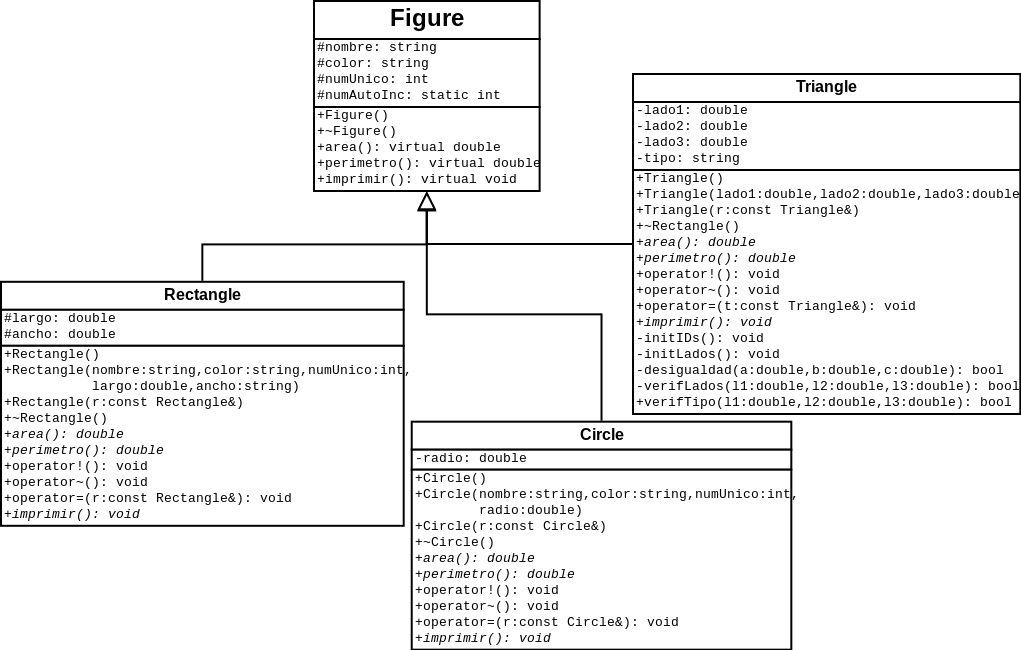
\includegraphics[width=\textwidth]{imgs/Labo3/Diagram1.png}
  \caption{Diagrama de clases}
  \label{fig:dia}
\end{figure}

%%%%%%%%%%%%%%%%%%%%%%%%%%%%%%%%%%%%%%%%%%%%%%%%%%%%%%%%%%%%%%%%%%%%%%%%%%%%%%%%%%%%%%%%%%%%%%%%%%%
\newpage
\section{Resultados}
%%%%%%%%%%%%%%%%%%%%%%%%%%%%%%%%%%%%%%%%%%%%%%%%%%%%%%%%%%%%%%%%%%%%%%%%%%%%%%%%%%%%%%%%%%%%%%%%%%%
Para observar los resultados de la implementación de las clases descritas, se creó un programa \texttt{main} en el que se crean algunos objetos. 

Para comprobar la funcionalidad de la clase \texttt{Circle}, se crea un objeto con el constructor vacío, lo cual causa que el programa solicite al usuario que ingrese los valores de los atributos:

\begin{minted}[linenos,autogobble,bgcolor=bg,breaklines,fontsize=\footnotesize ]{c++}
Circle circulo1 = Circle();
\end{minted}

Luego de esto se imprime los datos de información de la figura, área y perímetro, haciendo uso de la sobrecarga de los operadores $!$ y $\sim$. Posteriormente, se crea otra clase, pero esta vez pasándole los parámetros de los atributos a través del constructor:

\begin{minted}[linenos,autogobble,bgcolor=bg,breaklines,fontsize=\footnotesize ]{c++}
Circle circulo2("Circulo #2","Rojo",3,3.4);
\end{minted}

Por último, se comprueba el resultados de sobrecargar el operador = al igualar el primer circulo creado con el segundo. Los resultados de estas pruebas se pueden ver en la Figura \ref{fig:CIRC}.

\begin{figure}[H]
\centering
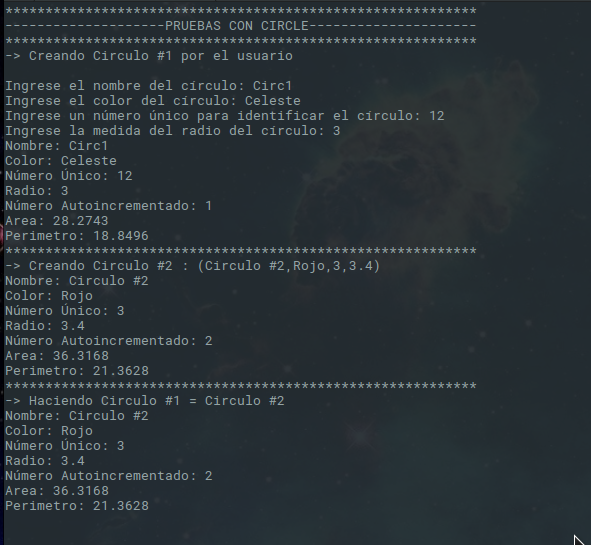
\includegraphics[width=.7\textwidth]{imgs/Labo3/CIRC}
\caption{Resultado de la implementación de la clase \texttt{Circle}}
\label{fig:CIRC}
\end{figure}

Una prueba similar se realizó para comprobar las funcionalidad de la clase \texttt{Rectangle} y los resultados se pueden ver en la Figura \ref{fig:RECT}.

\begin{figure}[H]
\centering
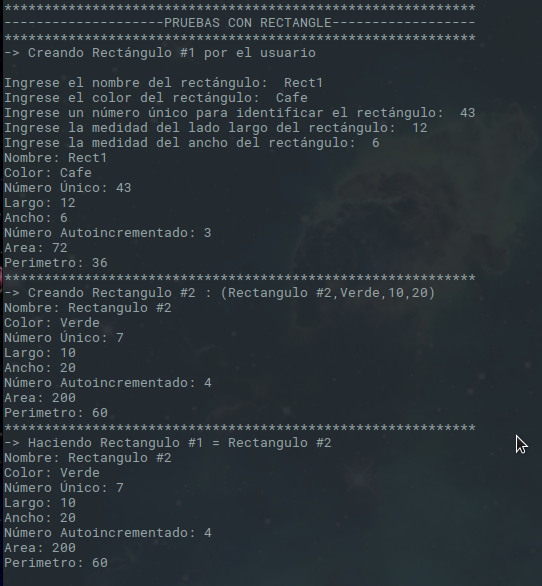
\includegraphics[width=.7\textwidth]{imgs/Labo3/RECT}
\caption{Resultado de la implementación de la clase \texttt{Rectangle}}
\label{fig:RECT}
\end{figure}

En la clase \texttt{Triangle}, también se hace una verificación para comprobar que los datos ingresados son válidos. En la Figura \ref{fig:TRI1}, se logra observar que si se ingresa lados que no cumplen para ser un triángulo, se solicita al usuario volver a ingresar datos.

\begin{figure}[H]
\centering
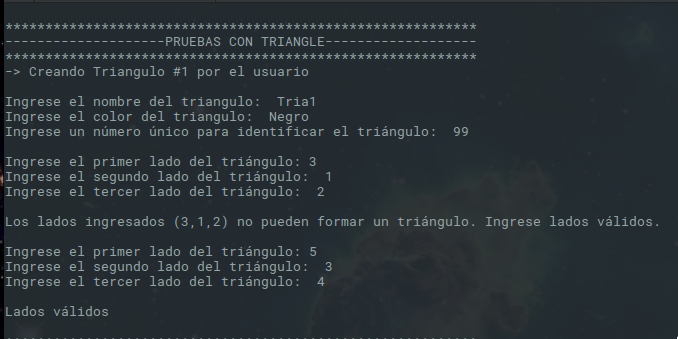
\includegraphics[width=.7\textwidth]{imgs/Labo3/TRI1}
\caption{Resultado de la implementación de la clase \texttt{Triangle}}
\label{fig:TRI1}
\end{figure}

Por último, se realizó la misma que para el círculo y rectángulo y los resultados se pueden ver en la Figura \ref{fig:TRI2}.

\begin{figure}[H]
\centering
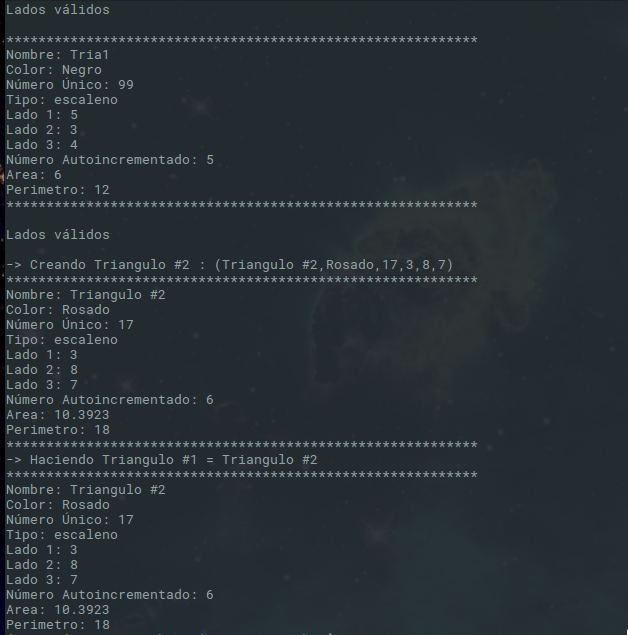
\includegraphics[width=.7\textwidth]{imgs/Labo3/TRI2}
\caption{Resultado de la implementación de la clase \texttt{Triangle}}
\label{fig:TRI2}
\end{figure}

Para correr toda la prueba es necesario ejecutar en la terminal el siguiente comando:

\begin{minted}[linenos,autogobble,bgcolor=bg,breaklines,fontsize=\footnotesize ]{bash}
make test
\end{minted}

%%%%%%%%%%%%%%%%%%%%%%%%%%%%%%%%%%%%%%%%%%%%%%%%%%%%%%%%%%%%%%%%%%%%%%%%%%%%%%%%%%%%%%%%%%%%%%%%%%%
\newpage
\section{Conclusiones}
 Como conclusiones se tiene que:
 
\begin{itemize}
\item A partir de una clase base se logra crear clases derivadas que contienen métodos y atributos heredados de la clase base, con esto se logra comprender el concepto de herencia en programación orientada a objetos.
\item Se implementó cuatro clases, con las cuales se logra crear círculos, rectángulos y triángulos y calcular su respectiva área y perímetro. 
\item Se logra sobrecargar operadores para darles diferentes usos y simplificar así la notación de las operaciones con objetos.
\item Se crea un diagrama UML con ejemplifica de mejor manera la jerarquía de las cuatro clases creadas en este proyecto.
\end{itemize}
%%%%%%%%%%%%%%%%%%%%%%%%%%%%%%%%%%%%%%%%%%%%%%%%%%%%%%%%%%%%%%%%%%%%%%%%%%%%%%%%%%%%%%%%%%%%%%%%%%%


%%%%%%%%%%%%%%%%%%
%--> LABORATORIO 4
%%%%%%%%%%%%%%%%%%
%%%%%%%%%%%%%%%%%%%%%%%%%%%%%%%%%%%%%%%%%%%%%%%%%%%%%%%%%%%%%%%
% --> INTRODUCCIÓN
%%%%%%%%%%%%%%%%%%%%%%%%%%%%%%%%%%%%%%%%%%%%%%%%%%%%%%%%%%%%%%
\section{Introducción}

Según \cite{R1} la programación genérica está mucho más centrada en los algoritmos que en los datos, y su postulado fundamental puede sintetizarse en una palabra: generalización. Significa que, en la medida de lo posible, los algoritmos deben ser parametrizados al máximo y expresados de la forma más independiente posible de detalles concretos, permitiendo así que puedan servir para la mayor variedad posible de tipos y estructuras de datos.

%%%%%%%%%%%%%%%%%%%%%%%%%%%%%%%%%%%%%%%%%%%%%%%%%%%%%%%%%%%%%%
% --> OBJETIVOS
%%%%%%%%%%%%%%%%%%%%%%%%%%%%%%%%%%%%%%%%%%%%%%%%%%%%%%%%%%%%%%
\subsection{Objetivos}

A continuación, se enlistan los objetivos de este laboratorio.

%%%%%%%%%%%%%%%%%%%%%%%%%%%%%%%%%%%%%%%%%%%%%%%%%%%%%%%%%%%%%%
% --> OBJETIVO GENERAL
%%%%%%%%%%%%%%%%%%%%%%%%%%%%%%%%%%%%%%%%%%%%%%%%%%%%%%%%%%%%%%
\subsubsection{Objetivo General}
\begin{itemize}
\item Diseñar una serie de clases con plantillas que permitan hacer operaciones básicas con enteros. reales, fracciones, polinomios y matrices.
\end{itemize}

%%%%%%%%%%%%%%%%%%%%%%%%%%%%%%%%%%%%%%%%%%%%%%%%%%%%%%%%%%%%%%
% --> OBJETIVOS ESPECÍFICOS
%%%%%%%%%%%%%%%%%%%%%%%%%%%%%%%%%%%%%%%%%%%%%%%%%%%%%%%%%%%%%%
\subsubsection{Objetivos Específicos}
\begin{itemize}
\item 
\item 
\item 
\end{itemize}

%%%%%%%%%%%%%%%%%%%%%%%%%%%%%%%%%%%%%%%%%%%%%%%%%%%%%%%%%%%%%%
% --> ENUNCIADO
%%%%%%%%%%%%%%%%%%%%%%%%%%%%%%%%%%%%%%%%%%%%%%%%%%%%%%%%%%%%%%
\newpage

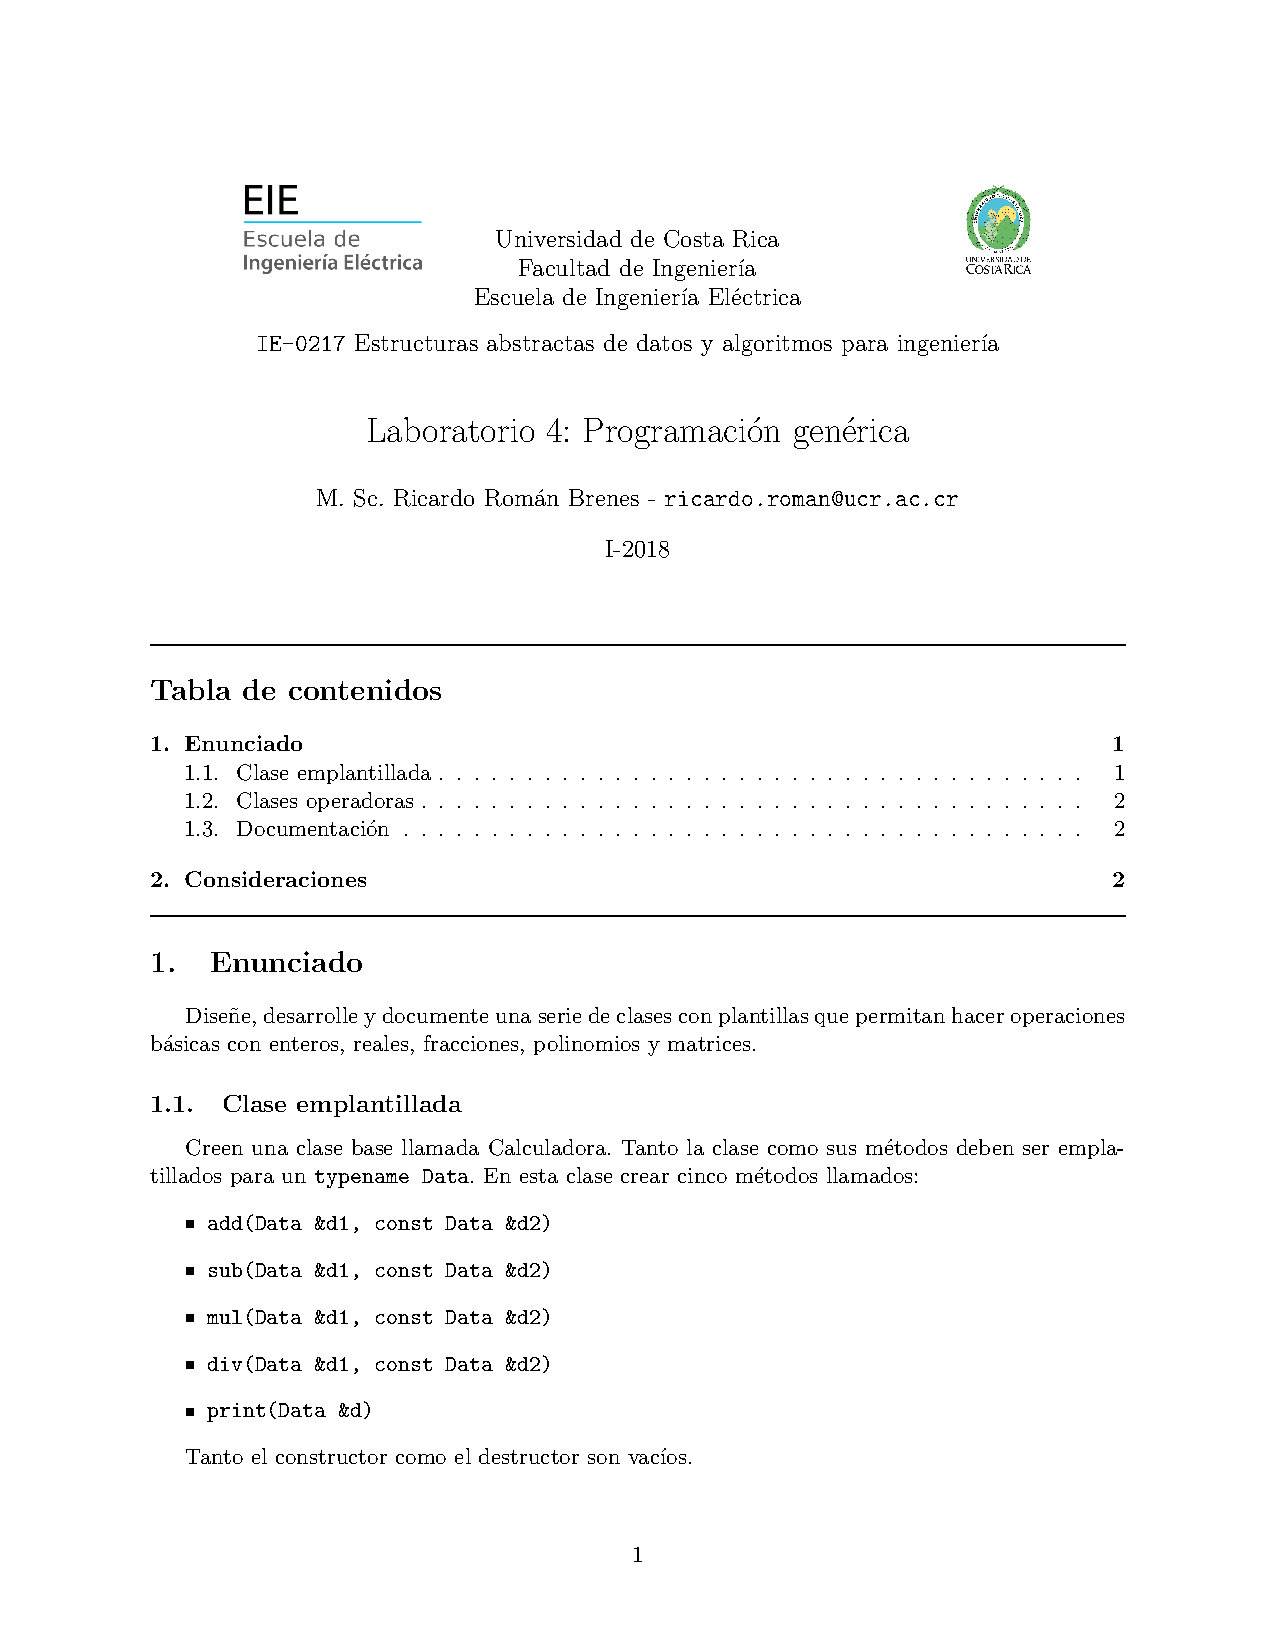
\includepdf[pages=1,pagecommand=\section{Enunciado}, scale=0.8]{enunciados/enun4} 
\includepdf[pages=2,pagecommand={},scale=0.8]{enunciados/enun4}

%%%%%%%%%%%%%%%%%%%%%%%%%%%%%%%%%%%%%%%%%%%%%%%%%%%%%%%%%%%%%%
% --> SOLUCIÓN
%%%%%%%%%%%%%%%%%%%%%%%%%%%%%%%%%%%%%%%%%%%%%%%%%%%%%%%%%%%%%%
\section{Solución}

%%%%%%%%%%%%%%%%%%%%%%%%%%%%%%%%%%%%%%%%%%%%%%%%%%%%%%%%%%%%%%
% --> CLASE POLINOMIO
%%%%%%%%%%%%%%%%%%%%%%%%%%%%%%%%%%%%%%%%%%%%%%%%%%%%%%%%%%%%%%
\subsection{Clase Polinomio}

La clase \texttt{Polynomial} realiza operaciones básicas de polinomios de grado n. En este archivo \texttt{.h} se declaran todas las funciones necesarias, así como dos variables necesarias para la ejecución, una tipo \texttt{int} para almacenar el tamaño del polinomio, es decir, la cantidad de coeficientes que posee. Y otra variable tipo \texttt{double*} para almacenar estos coeficientes, esto es un puntero que básicamente funciona como un \texttt{array}.

\begin{minted}[linenos,autogobble,bgcolor=bg,breaklines,fontsize=\footnotesize ]{c++}
class Polynomial
{
	public:
		Polynomial	(int Grado,double Coeficientes[]);
		Polynomial	(const Polynomial &l_cCopyPolynomial);
		~Polynomial	();
		Polynomial 	operator+(const Polynomial &P);
		Polynomial 	operator-(const Polynomial &P);
		Polynomial 	operator*(const Polynomial &P);
		Polynomial	operator/(const Polynomial &P);
		void 				operator~(void);
	protected:
		double* m_pCoefPolinomio;
	private:
		int m_iTamPolinomio;

};

\end{minted}

\subsubsection{Métodos de \texttt{Polynomial()}.}
\begin{itemize}
    \item \textbf{Método constructor:}
    
    El método constructor por defecto requiere de dos argumentos, uno es el grado del polinomio, y el otro es un arreglo del tipo \texttt{double} con los coeficientes que conforman el polinomio.  
\end{itemize}

%%%%%%%%%%%%%%%%%%%%%%%%%%%%%%%%%%%%%%%%%%%%%%%%%%%%%%%%%%%%%%
% --> CLASE FRACCIÓN
%%%%%%%%%%%%%%%%%%%%%%%%%%%%%%%%%%%%%%%%%%%%%%%%%%%%%%%%%%%%%%
\subsection{Clase Fracción}

\begin{minted}[linenos,autogobble,bgcolor=bg,breaklines,fontsize=\footnotesize ]{c++}
class Fraction
{
	public:
		Fraction();
		Fraction(int l_iNum, int l_iDen);
		Fraction(const Fraction &l_cCopyFraction);
		~Fraction();
		Fraction operator+(const Fraction &rhs);
		Fraction operator-(const Fraction &rhs);
		Fraction operator*(const Fraction &rhs);
		Fraction operator/(const Fraction &rhs);
		void operator~();
	protected:
	private:
		int m_iNumerador;
		int m_iDenominador;
		void checkDen();
};
\end{minted}


%%%%%%%%%%%%%%%%%%%%%%%%%%%%%%%%%%%%%%%%%%%%%%%%%%%%%%%%%%%%%%
% --> CLASE MATRIZ
%%%%%%%%%%%%%%%%%%%%%%%%%%%%%%%%%%%%%%%%%%%%%%%%%%%%%%%%%%%%%%
\subsection{Clase Matriz}

\begin{minted}[linenos,autogobble,bgcolor=bg,breaklines,fontsize=\footnotesize ]{c++}
class Matrix
{
	public:
		Matrix		(int l_iRowSize, int l_iColSize, bool l_bFlag);
		Matrix		(double* l_pMatrix, int l_iRowSize, int l_iColSize);
		Matrix		(const Matrix &l_cCopyMat);
		~Matrix		();
		Matrix 		operator+(const Matrix &rhs);
		Matrix 		operator-(const Matrix &rhs);
		Matrix 		operator*(const Matrix &rhs);
		Matrix 		operator/(const Matrix &rhs);
		int 			GetRowSize();
		int 			GetColsSize();
		double 		GetMatValue(int l_iRow, int l_iCol);
		void  		SetMatValue(int l_iRC, double l_dValue);
		void 			operator~(void);
	protected:
	private:
		double* 	m_pMatrix;
		int 			m_iRows;
		int 			m_iCols;
};
\end{minted}

%%%%%%%%%%%%%%%%%%%%%%%%%%%%%%%%%%%%%%%%%%%%%%%%%%%%%%%%%%%%%%
% --> CLASE CALCULADORA
%%%%%%%%%%%%%%%%%%%%%%%%%%%%%%%%%%%%%%%%%%%%%%%%%%%%%%%%%%%%%%
\subsection{Clase Calculadora}

\begin{minted}[linenos,autogobble,bgcolor=bg,breaklines,fontsize=\footnotesize ]{c++}
#ifndef CALCULATOR_H
#define CALCULATOR_H

#include <iostream>
#include <string>
#include <math.h>
#include "fraction.h"
#include "matrix.h"
#include "polynomial.h"

using namespace std;

template<typename Data>
class Calculator
{
	public:
		Calculator(){};
		~Calculator(){};
		Data add(Data &d1, const Data &d2) {return d1+d2;};
		Data sub(Data &d1, const Data &d2) {return d1-d2;};
		Data mul(Data &d1, const Data &d2) {return d1*d2;};
		Data div(Data &d1, const Data &d2) {return d1/d2;};
		void print(Data &d){~d;};
	protected:
	private:
};

#endif //CALCULATOR_H
\end{minted}

%%%%%%%%%%%%%%%%%%%%%%%%%%%%%%%%%%%%%%%%%%%%%%%%%%%%%%%%%%%%%%
% --> MAIN
%%%%%%%%%%%%%%%%%%%%%%%%%%%%%%%%%%%%%%%%%%%%%%%%%%%%%%%%%%%%%%
\subsection{Programa Principal}

\begin{minted}[linenos,autogobble,bgcolor=bg,breaklines,fontsize=\footnotesize ]{c++}
class Matrix
{
	public:
		Matrix		(int l_iRowSize, int l_iColSize, bool l_bFlag);
		Matrix		(double* l_pMatrix, int l_iRowSize, int l_iColSize);
		Matrix		(const Matrix &l_cCopyMat);
		~Matrix		();
		Matrix 		operator+(const Matrix &rhs);
		Matrix 		operator-(const Matrix &rhs);
		Matrix 		operator*(const Matrix &rhs);
		Matrix 		operator/(const Matrix &rhs);
		int 			GetRowSize();
		int 			GetColsSize();
		double 		GetMatValue(int l_iRow, int l_iCol);
		void  		SetMatValue(int l_iRC, double l_dValue);
		void 			operator~(void);
	protected:
	private:
		double* 	m_pMatrix;
		int 			m_iRows;
		int 			m_iCols;
};
\end{minted}

%%%%%%%%%%%%%%%%%%%%%%%%%%%%%%%%%%%%%%%%%%%%%%%%%%%%%%%%%%%%%%
% --> RESULTADOS
%%%%%%%%%%%%%%%%%%%%%%%%%%%%%%%%%%%%%%%%%%%%%%%%%%%%%%%%%%%%%%
\section{Resultados}


%%%%%%%%%%%%%%%%%%%%%%%%%%%%%%%%%%%%%%%%%%%%%%%%%%%%%%%%%%%%%%
% --> CONCLUSIONES
%%%%%%%%%%%%%%%%%%%%%%%%%%%%%%%%%%%%%%%%%%%%%%%%%%%%%%%%%%%%%%
\section{Conclusiones}


Como conclusiones se tiene que:

\begin{itemize}
\item fd
\end{itemize}


%%%%%%%%%%%%%%%%%%%%%%%%%%%%%%%%%%%%%%%%%%%%%%%%%%%%%%%%%%%%%%
% --> BIBLIOGRAFIA
%%%%%%%%%%%%%%%%%%%%%%%%%%%%%%%%%%%%%%%%%%%%%%%%%%%%%%%%%%%%%%
\begin{thebibliography}{IEEE}
\bibitem{R1} Talens, S. \textbf{\textit{Curso de programación en C++}}. EUI (UPV) Valencia, 17 al 28 de Julio de 1995. 
\end{thebibliography}


%%%%%%%%%%%%%%%%%%
%--> PROPUESTA PROYECTO 0
%%%%%%%%%%%%%%%%%%
%%%%%%%%%%%%%%%%%%%%%%%%%%%%%%%%%%%%%%%%%%%%%%%%%%%%%%%%%%%%%%%
% --> ENUNCIADO
%%%%%%%%%%%%%%%%%%%%%%%%%%%%%%%%%%%%%%%%%%%%%%%%%%%%%%%%%%%%%%
\section{Enunciado}
El objetivo de este proyecto es familiarizar al estudiante con la programación forma de una estructura de datos básica y/o algoritmo en el lenguaje C++, así como su análisis y presentación. Particularmente en este proyecto se crearan imágenes digitales a partir de archivos binarios.

Se deben tomar archivos binarios de cualquier  índole y calcular el tamaño máximo que puede crearse con sus bytes una imagen X × Y píxeles (no necesariamente cuadrada), tomando en cuenta que cada píxel de dicha imagen esta representado por 3 bytes que representan intensidad de colores rojo, verde y azul, cuyos valores varían entre 0 y 255. Su programa debe tener la capacidad de escribir imágenes en formatos PNG, JPEG, GIF, BMP. Puede utilizar bibliotecas de terceros para implementar esta ultima funcionalidad.
%%%%%%%%%%%%%%%%%%%%%%%%%%%%%%%%%%%%%%%%%%%%%%%%%%%%%%%%%%%%%%
% --> RESEÑA DEL ALGORITMO/ESTRUCTURA
%%%%%%%%%%%%%%%%%%%%%%%%%%%%%%%%%%%%%%%%%%%%%%%%%%%%%%%%%%%%%%
\section{Reseña del algoritmo/estructura}

Una imagen digital en formato RGB se forma por combinación de tres canales. Cada canal se corresponde con un color primario: Red (rojo), Green (verde), y Blue (azul), en donde se asigna un valor de intensidad a cada color que oscila entre 0 y 255, por lo que cada valor de color debe ser guardo en 8 bits o un byte. De la combinación surgen hasta 16,7 millones de colores, que son capaces de describir la mayoría de las imágenes a nivel digital.

En la figura \ref{fig:matrizRGB}, se puede observar con mayor claridad este concepto.

\begin{figure}[H]
\centering
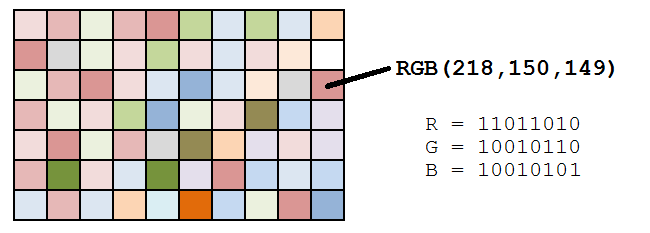
\includegraphics[width=0.6\textwidth]{imgs/proyecto0/matrix.png}
\caption{Imágenes en formato PNG}
\label{fig:matrizRGB}
\end{figure}

Existen en la actualidad una gran cantidad de formatos de archivo que permiten visualizar imágenes digitales que utilizan el mapeo RGB. Esto permite que sea posible implementar algún método que convierta un archivo binario, extrayendo su información en forma de bits puros, mapearlo a RGB, y presentarlo en uno de estos  estándar, de manera que se pueda visualizar con algún dispositivo digital capaz de abrir la imagen. Entre los estándares más comunes se encuentran BMP, PNG, JPG y GIF.

%ESTO SUENA RARO, VOY A TRATAR DE REFRASEARLO   Para generar estas imágenes a partir de un archivo binario de 1 y 0, existen en la actualidad una gran cantidad de formatos de imágenes que nos permite pasar de un archivo binario a una imagen con un formato estándar el cual se puede visualizar con algún dispositivo digital capaz de abrir la imagen con un formato especifico>>> NO LO SÉ, RICK. Entre los estándares más comunes se encuentran BMP, PNG, JPG y GIF. 

A continuación se presenta una breve descripición de las características básicas de los distintos formatos de imagénes que se pretenden usar en este proyecto:

\begin{itemize}
    \item \textbf{PNG}: Las imágenes \textit{Portable Network Graphics}, según \cite{R2} es un formato de imagen sin pérdida que se publicó en 1996. PNG no se diseñó para uso profesional, sino para transferir imágenes en Internet, y solo admite imágenes de nivel de grises e imágenes rgb (también imágenes de color basadas en paletas).
    %---------------------------------------------------------------------
    \item \textbf{JPEG}: Los archivos en formato \textit{Joint Photographic Experts Group}, según \cite{R2} es un formato de imagen que fue aprobado como estándar internacional en 1994. JPEG es usualmente con pérdida, pero también puede ser sin pérdida y se ha convertido en un formato popular para la representación de imágenes en Internet. El estándar define tanto los algoritmos para codificar y decodificar como formato de almacenamiento. JPEG divide la imagen en bloques de 8 × 8 y transforma cada bloquear con una Transformada de Coseno Discreta. Estos valores corresponden a valores más altos 359 frecuencias (variaciones rápidas de color) se establecen en 0 a menos que sean bastante grande, ya que esto no se nota mucho por la percepción humana. Los valores DCT perturbados luego están codificados por una variación de la codificación de Huffman. JPEG también puede usar aritmética codificación, pero esto aumenta los tiempos de codificación y decodificación, con solo alrededor del $\percent[5]$ de mejora en la relación de compresión. El nivel de compresión en imágenes JPEG es seleccionado por el usuario y puede resultar en artefactos conspicuos
    si está configurado demasiado alto. JPEG es especialmente propenso a artefactos en áreas donde la intensidad cambia rápidamente de píxel a píxel. La extensión de un archivo JPEG es .jpg o .jpeg
    %---------------------------------------------------------------------
    \item \textbf{GIF}: El formato \textit{Graphics Interchange Format} fue desarrollado en 1987 por CompuServe Incorporated, principalmente para su uso en Internet. Según \cite{R3}, este formato admite profundidades de color de 1 bit (monocromo) a 8 bits (256 colores) y almacena siempre las imágenes en forma comprimida, utilizando compresión LZW sin pérdida. Otras características compatibles incluyen entrelazado y transparencia.
    %---------------------------------------------------------------------
    \item \textbf{BMP}: El formato \textit{BitMap} fue desarrollado por Microsoft como el formato nativo del sistema operativo Windows. Las versiones del formato han coincidido con las versiones de Windows, la primera versión que aparece en 1985 con Windows 1.0. Según \cite{R3} es un formato  que admite profundidades de color de 1 bit a 32 bits y proporciona compresión RLE opcional sin pérdida.
\end{itemize}

En el cuadro \ref{T:T111}, se muestra un resumen de los distintos formatos: 

\begin{table}[H]
\begin{center}
    \begin{tabular}{ |>{\centering\arraybackslash}m{4cm}|>{\centering\arraybackslash}m{5.5cm}|>{\centering\arraybackslash}m{5.5cm}| }
    	\hline
    	\cellcolor{cl} \textbf{Formato} & \cellcolor{cl} \textbf{Ventajas} & \cellcolor{cl} \textbf{Desventajas}\\ \hline \hline
    	PNG (\textit{Portable Network Graphics}) & Es mejor cuando la imagen tiene grandes áreas uniformemente coloreadas; robusto& Muchos navegadores antiguos actualmente no son compatibles con el formato de archivo PNG. \\
    	\hline
    	JPEG (\textit{Joint Photographic Experts Group}) & Pequeños archivos: la compresión no afecta de manera apreciable la calidad de la imagen & - \\
    	\hline
    	GIF (\textit{Graphics Interchange Format}) & Soporta animaciones & Limitado a 256 colores, sin función real en comparación con otros formatos.\\
    	\hline
    	BMP (\textit{BitMap}) &Son ampliamente usados en los programas de Windows&Son archivos grandes y sin comprimir.\\
    	\hline
    \end{tabular}
\end{center}
\label{T:T111}
\caption{Resumen de características de los formatos de imágenes. \cite{R1}}
\end{table}


%%%%%%%%%%%%%%%%%%%%%%%%%%%%%%%%%%%%%%%%%%%%%%%%%%%%%%%%%%%%%%
% --> FUNCIONAMIENTO DEL ALGORITMO
%%%%%%%%%%%%%%%%%%%%%%%%%%%%%%%%%%%%%%%%%%%%%%%%%%%%%%%%%%%%%%
\section{Funcionamiento del algoritmo/estructura}
El programa constará de varias clases y métodos para la lectura, traducción y escritura. Se utilizará una estructura de herencia, donde se tendrán las siguientes clases y métodos:
%------------------------------
\subsection{Clase Base Píxeles}
%------------------------------
Esta clase contendrá un método encargado de leer un archivo .txt con la ruta del archivo de entrada que contiene los datos en binario del código que se quiere representar mediante una imagen. Con este código también se calcula el tamaño en bytes del archivo de entrada, para esto se utilizará una biblioteca como \texttt{fstream} con su método \texttt{read()}, o bien utilizando la función \texttt{stat} de la biblioteca \texttt{sys/stat.h}. Una vez se tenga lo anterior, se almacenarán los datos de la hilera de entrada en un arreglo o vector, sobre el cual se trabajará. Por tal razón, es posible que esta clase cuente con los siguientes métodos:

    
\begin{itemize}
    %\item \textbf{Clase base:} 
    %Esta clase contendrá un método encargado de leer un archivo .txt con la ruta del archivo de entrada que contiene los datos en binario del código que se quiere representar mediante una imagen. Con este código también se calcula el tamaño en bytes del archivo de entrada, para esto se utilizará una biblioteca como \texttt{fstream} con su método \texttt{read()}, o bien utilizando la función \texttt{stat} de la biblioteca \texttt{sys/stat.h} \cite{R7}. Una vez se tenga lo anterior, se almacenarán los datos de la hilera de entrada en un arreglo o vector, sobre el cual se trabajará. 
    \item \textbf{Método de formato:} 
    Esta función tomará el arreglo a trabajar y calculará si tiene el tamaño suficiente para generar una imagen, además definirá la relación de aspecto de la imagen . Los formatos a utilizar serán los más comunes, como lo son 16:9, 4:3, 3:2 y 1:1. En caso de que se tenga una cantidad suficiente de bytes para generar la imagen, pero falten o sobren datos, se truncará el arreglo, y se eliminarán los últimos bytes de éste.
    \item \textbf{Método del algoritmo de traducción:} Esta función será la más importante debido a que es la encargada de traducir de un binario a una imagen. Para la traducción se utilizará el modelo RGB, en donde las imágenes son representadas por los colores rojo, verde y azul. Cada uno de estos colores se representa con un número binario que va de 0 a 255 en base decimal, o en binario, de 00000000 a 11111111 \cite{R5}. El valor más bajo representa la tonalidad más oscura del color, y el valor más alto representa la tonalidad más clara. Para la traducción se tomará el arreglo y se analizará, bloques de 24bits, o lo que es lo mismo, 3 bytes consecutivos. Cada triada se tomará de manera que los primeros 8 bits en binario sean la tonalidad de rojo; los siguientes 8 bits la tonalidad verde y los siguientes la tonalidad en azul. Cada triada con sus respectivos tres valores RGB corresponde a un píxel de la imagen. Una vez que se completa la traducción, el método devuelve un arreglo o hilera RGB listo para su representación visual.
    %\item \textbf{Generación de la imagen:} 
\end{itemize}

%Las clases derivadas deben ser capaces 

%------------------------------
\subsection{Clase Derivada BMP} 
%------------------------------

Esta clase debe ser capaz de tomar el unsigned char *rgb o el archivo binario ya convertido en formato RGB y guardarlo en una ruta especificada por la string filename. Según la investigación realiada, para lograr esto se deben definir los atributos necesarios del header de un archivo en formato BMP y además esta clase debe ser capaz de lograr al menos el siguiente método:
 
\begin{itemize}
    \item \textbf{Método guardar array RGB en formato BMP}: este método debe ser capaz de tomar los atributos de esta clase y hacer uso de la función \texttt{fwrite()}, lograr escribir la imagen en formato BMP.
\end{itemize}

En este caso no es necesario usar una biblioteca de terceros, ya que todas las funciones necesarias se encuentran dentro de las librería estandar de C++, esto se puede ya que este formato no hace de ningún método de comprensión de los datos para generar la imagen. 

%------------------------------
\subsection{Clase Derivada PNG}
%------------------------------

Esta clase contiene funciones capaces de trabajar el formato PNG. Para esto se puede utilizar la biblioteca \texttt{libpng}.

\begin{itemize}
    \item \textbf{Método guardar array RGB en formato PNG}: este método debe ser capaz de abrir en el archivo RGB del espacio de trabajo mediante un puntero, debe crear la imagen y guardarla.
\end{itemize}

% PNG -> libpng-dev -> sudo apt-get install libpng-dev \cite{R6}

%------------------------------
\subsection{Clase Derivada JPEG}
%------------------------------
Esta clase contiene funciones capaces de trabajar el formato JPEG con su algoritmo de compresión. Para esto se puede utilizar la biblioteca \texttt{libjpeg}, toda esta biblioteca está escrita completamente en C, por lo que su uso en C++ no debe de generar problemas.

\begin{itemize}
    \item \textbf{Método guardar array RGB en formato JPEG}: este método debe ser capaz de abrir en el archivo RGB del espacio de trabajo mediante un puntero y aplicarle la compresión de acuerdo a la calidad deseada. Al final debe crear la imagen y guardarla.
\end{itemize}

% PNG -> libjpeg-dev -> sudo apt-get install libjpeg-dev 

%------------------------------
\subsection{Clase Derivada GIF}
%------------------------------
Para implementar las funcionalidades de esta clase se puede utilizar la biblioteca \texttt{Magick++}. Ésta es parte del paquete \texttt{ImageMagick}, y provee una muy amplia gama de clases y métodos para trabajar con imágenes, y soporta gran cantidad de formatos. En este caso, nos interesa generar una imagen en formato GIF a partir del arreglo de pixeles obtenido anteriormente.

Otra alternativa es utilizar la biblioteca \texttt{giflib}, que permite convertir directamente imágenes en formato GIF a tripletas RGB de 24 bits y viceversa \cite{R8}.

\begin{itemize}
    \item \textbf{Método guardar array RGB en formato GIF}: Si se utiliza la herramienta \texttt{Magick++}, es posible crear un objeto de la clase \texttt{Image}, pasándole como parámetros sus dimensiones, el formato de mapeo de los pixeles (en este caso, RGB), el tipo de dato que guarda los pixeles (float, char, integer...) y el arreglo de datos que generará la imagen \cite{R9}. 
\end{itemize}

%%%%%%%%%%%%%%%%%%%%%%%%%%%%%%%%%%%%%%%%%%%%%%%%%%%%%%%%%%%%%%
% --> EXPERIMENTOS QUE SE REALIZARAN
%%%%%%%%%%%%%%%%%%%%%%%%%%%%%%%%%%%%%%%%%%%%%%%%%%%%%%%%%%%%%%
\section{Experimentos que se realizarán}


Para comprobar la funcionalidad del programa se ejecutará varias veces con diferentes entradas. En donde se variará el largo del archivo binario para comprobar cómo responde y cómo maneja casos especiales como no tener una cantidad suficiente de bytes, también se probará la respuesta ante posibles casos de error como si se presentase un símbolo diferente a un 1 o un 0. 

Otra de las pruebas a realizar corresponde a generar desde un mismo archivo imágenes con diferentes dimensiones, si se tiene la cantidad suficiente de datos.

Un caso importante que experimentar es utilizar como base el mismo archivo binario para crear una imagen de las mismas dimensiones pero en cada uno de los distintos formatos BMP, JPEG, GIF y PNG, y así observar si se obtiene la misma imagen de salida o si se obtiene un resultado distinto.



%%%%%%%%%%%%%%%%%%%%%%%%%%%%%%%%%%%%%%%%%%%%%%%%%%%%%%%%%%%%%%
% --> BIBLIOGRAFIA
%%%%%%%%%%%%%%%%%%%%%%%%%%%%%%%%%%%%%%%%%%%%%%%%%%%%%%%%%%%%%%
\begin{thebibliography}{IEEE}
\bibitem{R1} Luca, M. \textbf{\textit{A Basic Summary of Image Formats}}.  Visto el 5 de Mayo del 2018 en: \url{http://www.student.montefiore.ulg.ac.be/~merciadri/docs/papers/image-formats.pdf}.

\bibitem{R2} Autor Desconocido. \textbf{\textit{Digital images and image formats}}. Visto el 5 de Mayo del 2018 en: \url{http://www.uio.no/studier/emner/matnat/math/MAT-INF1100/h08/kompendiet/images.pdf}.

\bibitem{R3} Brown, A. \textbf{\textit{Graphics File Formats}}. 2008. THe National Archives. Visto el 5 de Mayo del 2018 en: \url{https://www.nationalarchives.gov.uk/documents/graphic-file-formats.pdf}.

\bibitem{R4} PNG. \textit{\textbf{Official documentation of libpng}}. Visto el 5 de Mayo del 2018 en: \url{http://www.libpng.org/pub/png/libpng.html}. 

\bibitem{R5} Kumar, T. Verma, K. \textbf{\textit{A Theory Based on Conversion of RGB image to Gray
image}}. 2010. International Journal of Computer Applications, Vol. 7. No. 2. Visto el 5 de Mayo del 2018 en: \url{https://www.researchgate.net/profile/Karun_Verma/publication/46286639_A_Theory_Based_on_Conversion_of_RGB_image_to_Gray_image/links/5704a3b008ae44d70ee0662c.pdf}.

\bibitem{R6} Greensted, A. \textbf{\textit{Creating PNGs with libpng}}. Visto el 5 de Mayo del 2018 en: \url{http://www.labbookpages.co.uk/software/imgProc/libPNG.html}.

\bibitem{R7} Autor Desconocido. \textbf{\textit{C++ Binary File I/O}}. Visto el 5 de Mayo del 2018 en: \url{http://courses.cs.vt.edu/~cs2604/fall00/binio.html}

\bibitem{R8} Raymon, E. \textbf{\textit{Introduction to GIFLIB}}. Visto el 5 de Mayo del 2018 en: \url{http://giflib.sourceforge.net/intro.html}

\bibitem{R9} Autor desconocido. \textbf{\textit{Magick::Image Class}}. Visto el 5 de Mayo del 2018 en: \url{https://www.imagemagick.org/api/Image++.php}



\end{thebibliography}

%%%%%%%%%%%%%%%%%%
%--> LABORATORIO 5
%%%%%%%%%%%%%%%%%%
%%%%%%%%%%%%%%%%%%%%%%%%%%%%%%%%%%%%%%%%%%%%%%%%%%%%%%%%%%%%%%%%%%%%%%%%%%%%%%%%%%%%%%%%%%%%%%%%%%%%
\section{Introducción}
%%%%%%%%%%%%%%%%%%%%%%%%%%%%%%%%%%%%%%%%%%%%%%%%%%%%%%%%%%%%%%%%%%%%%%%%%%%%%%%%%%%%%%%%%%%%%%%%%%%


%%%%%%%%%%%%%%%%%%%%%%%%%%%%%%%%%%%%%%%%%%%%%%%%%%%%%%%%%%%%%%%%%%%%%%%%%%%%%%%%%%%%%%%%%%%%%%%%%%%
\subsection{Objetivos}
\begin{enumerate}
\item 
\item 
\item 
\item 
\end{enumerate}
%%%%%%%%%%%%%%%%%%%%%%%%%%%%%%%%%%%%%%%%%%%%%%%%%%%%%%%%%%%%%%%%%%%%%%%%%%%%%%%%%%%%%%%%%%%%%%%%%%%
\section{Enunciado}
%%%%%%%%%%%%%%%%%%%%%%%%%%%%%%%%%%%%%%%%%%%%%%%%%%%%%%%%%%%%%%%%%%%%%%%%%%%%%%%%%%%%%%%%%%%%%%%%%%%

%%%%%%%%%%%%%%%%%%%%%%%%%%%%%%%%%%%%%%%%%%%%%%%%%%%%%%%%%%%%%%%%%%%%%%%%%%%%%%%%%%%%%%%%%%%%%%%%%%%
\section{Solución}
%%%%%%%%%%%%%%%%%%%%%%%%%%%%%%%%%%%%%%%%%%%%%%%%%%%%%%%%%%%%%%%%%%%%%%%%%%%%%%%%%%%%%%%%%%%%%%%%%%%


\begin{minted}[linenos,autogobble,bgcolor=bg,breaklines,fontsize=\footnotesize ]{c++}
#include <string>
#include <iostream>
using namespace std;

class FileUtil
{
  public:
  	FileUtil(string s, ios_base::openmode p);
  	~FileUtil();
  	string read();
  	string* readLines();
  	int write(string s);
  	int write(string* s, int n);
    void countNumberLines();
    int getNumberLines();
  private:
    //Numero de lineas.
    int numLines;
    //Dirección de lectura.
    string ruta;
    //Modo de lectura.
  	ios_base::openmode modo;
    //Linea leida.
    string line;
    //Puntero con la direccion del arreglo de las lineas leidas.
    string* lines;

};
\end{minted}


%%%%%%%%%%%%%%%%%%%%%%%%%%%%%%%%%%%%%%%%%%%%%%%%%%%%%%%%%%%%%%%%%%%%%%%%%%%%%%%%%%%%%%%%%%%%%%%%%%%
\section{Resultados}
%%%%%%%%%%%%%%%%%%%%%%%%%%%%%%%%%%%%%%%%%%%%%%%%%%%%%%%%%%%%%%%%%%%%%%%%%%%%%%%%%%%%%%%%%%%%%%%%%%%


%%%%%%%%%%%%%%%%%%%%%%%%%%%%%%%%%%%%%%%%%%%%%%%%%%%%%%%%%%%%%%%%%%%%%%%%%%%%%%%%%%%%%%%%%%%%%%%%%%%
\section{Conclusiones}
%%%%%%%%%%%%%%%%%%%%%%%%%%%%%%%%%%%%%%%%%%%%%%%%%%%%%%%%%%%%%%%%%%%%%%%%%%%%%%%%%%%%%%%%%%%%%%%%%%%

%%%%%%%%%%%%%%%%%%
%--> LABORATORIO 6
%%%%%%%%%%%%%%%%%%
%%%%%%%%%%%%%%%%%%%%%%%%%%%%%%%%%%%%%%%%%%%%%%%%%%%%%%%%%%%%%%%
% --> INTRODUCCIÓN
%%%%%%%%%%%%%%%%%%%%%%%%%%%%%%%%%%%%%%%%%%%%%%%%%%%%%%%%%%%%%%
\section{Introducción}


%%%%%%%%%%%%%%%%%%%%%%%%%%%%%%%%%%%%%%%%%%%%%%%%%%%%%%%%%%%%%%
% --> OBJETIVOS
%%%%%%%%%%%%%%%%%%%%%%%%%%%%%%%%%%%%%%%%%%%%%%%%%%%%%%%%%%%%%%
\subsection{Objetivos}



%%%%%%%%%%%%%%%%%%%%%%%%%%%%%%%%%%%%%%%%%%%%%%%%%%%%%%%%%%%%%%
% --> OBJETIVO GENERAL
%%%%%%%%%%%%%%%%%%%%%%%%%%%%%%%%%%%%%%%%%%%%%%%%%%%%%%%%%%%%%%
\subsubsection{Objetivo General}
\begin{itemize}
\item 
\end{itemize}

%%%%%%%%%%%%%%%%%%%%%%%%%%%%%%%%%%%%%%%%%%%%%%%%%%%%%%%%%%%%%%
% --> OBJETIVOS ESPECÍFICOS
%%%%%%%%%%%%%%%%%%%%%%%%%%%%%%%%%%%%%%%%%%%%%%%%%%%%%%%%%%%%%%
\subsubsection{Objetivos Específicos}
\begin{itemize}
\item 
\item 
\item 
\item
\item 
\end{itemize}

%%%%%%%%%%%%%%%%%%%%%%%%%%%%%%%%%%%%%%%%%%%%%%%%%%%%%%%%%%%%%%
% --> ENUNCIADO
%%%%%%%%%%%%%%%%%%%%%%%%%%%%%%%%%%%%%%%%%%%%%%%%%%%%%%%%%%%%%%
%\newpage

%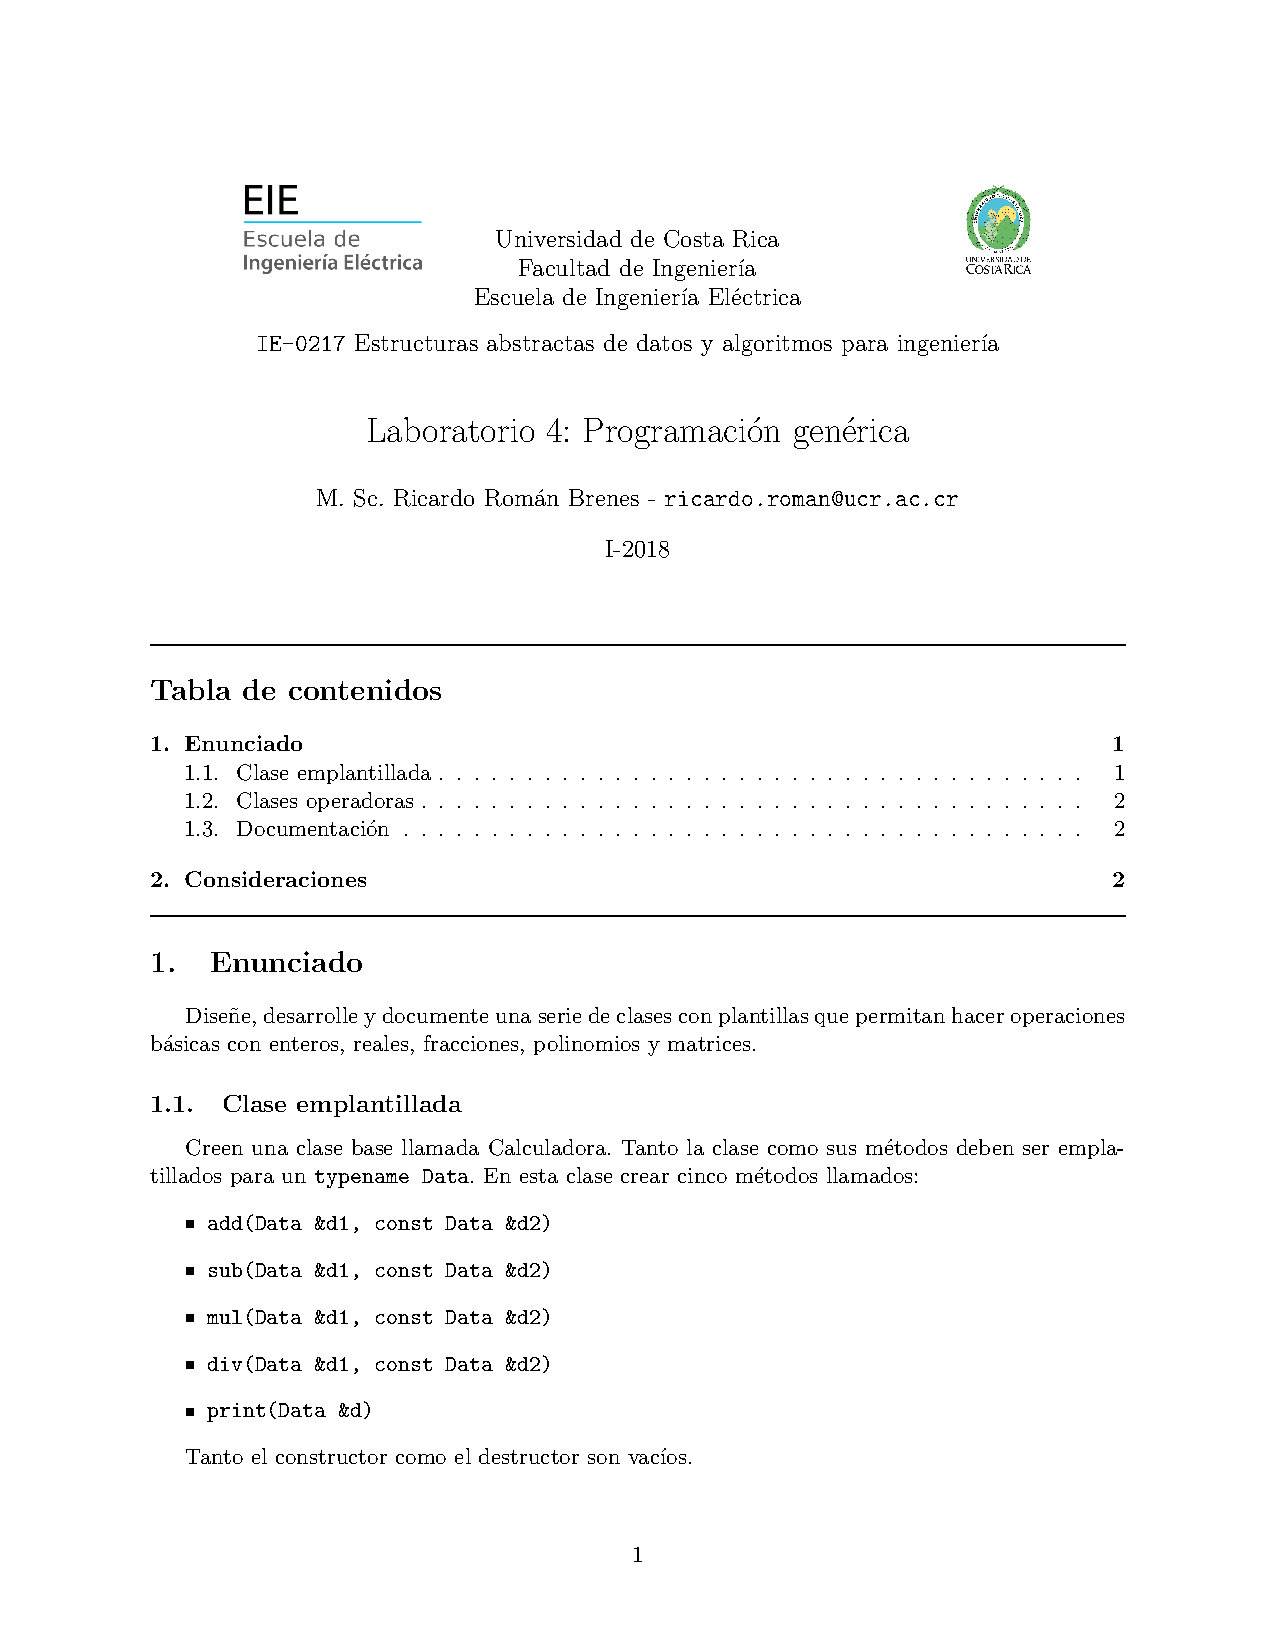
\includepdf[pages=1,pagecommand=\section{Enunciado}, scale=0.8]{enunciados/enun4} 
%\includepdf[pages=2,pagecommand={},scale=0.8]{enunciados/enun4}

%%%%%%%%%%%%%%%%%%%%%%%%%%%%%%%%%%%%%%%%%%%%%%%%%%%%%%%%%%%%%%
% --> SOLUCIÓN
%%%%%%%%%%%%%%%%%%%%%%%%%%%%%%%%%%%%%%%%%%%%%%%%%%%%%%%%%%%%%%
\section{Solución}


\begin{minted}[linenos,autogobble,bgcolor=bg,breaklines,fontsize=\footnotesize ]{c++}
#include <string>
#include <iostream>
using namespace std;

class FileUtil
{
  public:
  	FileUtil(string s, ios_base::openmode p);
  	~FileUtil();
  	string read();
  	string* readLines();
  	int write(string s);
  	int write(string* s, int n);
    void countNumberLines();
    int getNumberLines();
  private:
    //Numero de lineas.
    int numLines;
    //Dirección de lectura.
    string ruta;
    //Modo de lectura.
  	ios_base::openmode modo;
    //Linea leida.
    string line;
    //Puntero con la direccion del arreglo de las lineas leidas.
    string* lines;

};
\end{minted}



%%%%%%%%%%%%%%%%%%%%%%%%%%%%%%%%%%%%%%%%%%%%%%%%%%%%%%%%%%%%%%
% --> RESULTADOS
%%%%%%%%%%%%%%%%%%%%%%%%%%%%%%%%%%%%%%%%%%%%%%%%%%%%%%%%%%%%%%
\section{Resultados}



%%%%%%%%%%%%%%%%%%%%%%%%%%%%%%%%%%%%%%%%%%%%%%%%%%%%%%%%%%%%%%
% --> CONCLUSIONES
%%%%%%%%%%%%%%%%%%%%%%%%%%%%%%%%%%%%%%%%%%%%%%%%%%%%%%%%%%%%%%
\section{Conclusiones}


Como conclusiones se tiene que:

\begin{itemize}
\item 
\item 
\item 
\item 
\end{itemize}


%%%%%%%%%%%%%%%%%%%%%%%%%%%%%%%%%%%%%%%%%%%%%%%%%%%%%%%%%%%%%%
% --> BIBLIOGRAFIA
%%%%%%%%%%%%%%%%%%%%%%%%%%%%%%%%%%%%%%%%%%%%%%%%%%%%%%%%%%%%%%
\begin{thebibliography}{IEEE}
\bibitem{R1} Talens, S. \textbf{\textit{Curso de programación en C++}}. EUI (UPV) Valencia, 17 al 28 de Julio de 1995. 

\bibitem{R2} Raffo, E. \textbf{\textit{Programación genérica en C++, usando Metaprogramación}}. 2007. Sistemas de Informática. 
\end{thebibliography}



%%%%%%%%%%%%%%%%%%
%--> PROYECTO 0
%%%%%%%%%%%%%%%%%%
%%%%%%%%%%%%%%%%%%%%%%%%%%%%%%%%%%%%%%%%%%%%%%%%%%%%%%%%%%%%%%%
% --> ENUNCIADO
%%%%%%%%%%%%%%%%%%%%%%%%%%%%%%%%%%%%%%%%%%%%%%%%%%%%%%%%%%%%%%
\section{Enunciado}
El objetivo de este proyecto es familiarizar al estudiante con la programación forma de una estructura de datos básica y/o algoritmo en el lenguaje C++, así como su análisis y presentación. Particularmente en este proyecto se crearan imágenes digitales a partir de archivos binarios.

Se deben tomar archivos binarios de cualquier  índole y calcular el tamaño máximo que puede crearse con sus bytes una imagen X × Y píxeles (no necesariamente cuadrada), tomando en cuenta que cada píxel de dicha imagen esta representado por 3 bytes que representan intensidad de colores rojo, verde y azul, cuyos valores varían entre 0 y 255. Su programa debe tener la capacidad de escribir imágenes en formatos PNG, JPEG, GIF, BMP. Puede utilizar bibliotecas de terceros para implementar esta ultima funcionalidad.
%%%%%%%%%%%%%%%%%%%%%%%%%%%%%%%%%%%%%%%%%%%%%%%%%%%%%%%%%%%%%%
% --> RESEÑA DEL ALGORITMO/ESTRUCTURA
%%%%%%%%%%%%%%%%%%%%%%%%%%%%%%%%%%%%%%%%%%%%%%%%%%%%%%%%%%%%%%
\section{Reseña del algoritmo/estructura}

Una imagen digital en formato RGB se forma por combinación de tres canales. Cada canal se corresponde con un color primario: Red (rojo), Green (verde), y Blue (azul), en donde se asigna un valor de intensidad a cada color que oscila entre 0 y 255, por lo que cada valor de color debe ser guardo en 8 bits o un byte. De la combinación surgen hasta 16,7 millones de colores, que son capaces de describir la mayoría de las imágenes a nivel digital.

En la figura \ref{fig:matrizRGB}, se puede observar con mayor claridad este concepto.

\begin{figure}[H]
\centering
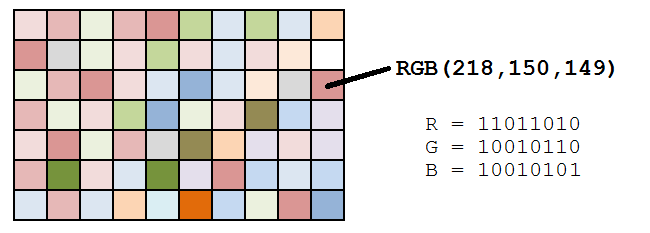
\includegraphics[width=0.6\textwidth]{imgs/proyecto0/matrix.png}
\caption{Imágenes en formato PNG}
\label{fig:matrizRGB}
\end{figure}

Existen en la actualidad una gran cantidad de formatos de archivo que permiten visualizar imágenes digitales que utilizan el mapeo RGB. Esto permite que sea posible implementar algún método que convierta un archivo binario, extrayendo su información en forma de bits puros, mapearlo a RGB, y presentarlo en uno de estos  estándar, de manera que se pueda visualizar con algún dispositivo digital capaz de abrir la imagen. Entre los estándares más comunes se encuentran BMP, PNG, JPG y GIF.

%ESTO SUENA RARO, VOY A TRATAR DE REFRASEARLO   Para generar estas imágenes a partir de un archivo binario de 1 y 0, existen en la actualidad una gran cantidad de formatos de imágenes que nos permite pasar de un archivo binario a una imagen con un formato estándar el cual se puede visualizar con algún dispositivo digital capaz de abrir la imagen con un formato especifico>>> NO LO SÉ, RICK. Entre los estándares más comunes se encuentran BMP, PNG, JPG y GIF. 

A continuación se presenta una breve descripción de las características básicas de los distintos formatos de imagénes que se pretenden usar en este proyecto:

\begin{itemize}
    \item \textbf{PNG}: Las imágenes \textit{Portable Network Graphics}, según \cite{R2} es un formato de imagen sin pérdida que se publicó en 1996. PNG no se diseñó para uso profesional, sino para transferir imágenes en Internet, y solo admite imágenes de nivel de grises e imágenes rgb (también imágenes de color basadas en paletas).
    %---------------------------------------------------------------------
    \item \textbf{JPEG}: Los archivos en formato \textit{Joint Photographic Experts Group}, según \cite{R2} es un formato de imagen que fue aprobado como estándar internacional en 1994. JPEG es usualmente con pérdida, pero también puede ser sin pérdida y se ha convertido en un formato popular para la representación de imágenes en Internet. El estándar define tanto los algoritmos para codificar y decodificar como formato de almacenamiento. JPEG divide la imagen en bloques de 8 × 8 y transforma cada bloquear con una Transformada de Coseno Discreta. Estos valores corresponden a valores más altos 359 frecuencias (variaciones rápidas de color) se establecen en 0 a menos que sean bastante grande, ya que esto no se nota mucho por la percepción humana. Los valores DCT perturbados luego están codificados por una variación de la codificación de Huffman. JPEG también puede usar aritmética codificación, pero esto aumenta los tiempos de codificación y decodificación, con solo alrededor del $\percent[5]$ de mejora en la relación de compresión. El nivel de compresión en imágenes JPEG es seleccionado por el usuario y puede resultar en artefactos conspicuos
    si está configurado demasiado alto. JPEG es especialmente propenso a artefactos en áreas donde la intensidad cambia rápidamente de píxel a píxel. La extensión de un archivo JPEG es .jpg o .jpeg
    %---------------------------------------------------------------------
    \item \textbf{GIF}: El formato \textit{Graphics Interchange Format} fue desarrollado en 1987 por CompuServe Incorporated, principalmente para su uso en Internet. Según \cite{R3}, este formato admite profundidades de color de 1 bit (monocromo) a 8 bits (256 colores) y almacena siempre las imágenes en forma comprimida, utilizando compresión LZW sin pérdida. Otras características compatibles incluyen entrelazado y transparencia.
    %---------------------------------------------------------------------
    \item \textbf{BMP}: El formato \textit{BitMap} fue desarrollado por Microsoft como el formato nativo del sistema operativo Windows. Las versiones del formato han coincidido con las versiones de Windows, la primera versión que aparece en 1985 con Windows 1.0. Según \cite{R3} es un formato  que admite profundidades de color de 1 bit a 32 bits y proporciona compresión RLE opcional sin pérdida.
\end{itemize}

En el cuadro \ref{T:T111}, se muestra un resumen de los distintos formatos: 

\begin{table}[H]
\begin{center}
    \begin{tabular}{ |>{\centering\arraybackslash}m{4cm}|>{\centering\arraybackslash}m{5.5cm}|>{\centering\arraybackslash}m{5.5cm}| }
    	\hline
    	\cellcolor{cl} \textbf{Formato} & \cellcolor{cl} \textbf{Ventajas} & \cellcolor{cl} \textbf{Desventajas}\\ \hline \hline
    	PNG (\textit{Portable Network Graphics}) & Es mejor cuando la imagen tiene grandes áreas uniformemente coloreadas; robusto& Muchos navegadores antiguos actualmente no son compatibles con el formato de archivo PNG. \\
    	\hline
    	JPEG (\textit{Joint Photographic Experts Group}) & Pequeños archivos: la compresión no afecta de manera apreciable la calidad de la imagen & - \\
    	\hline
    	GIF (\textit{Graphics Interchange Format}) & Soporta animaciones & Limitado a 256 colores, sin función real en comparación con otros formatos.\\
    	\hline
    	BMP (\textit{BitMap}) &Son ampliamente usados en los programas de Windows&Son archivos grandes y sin comprimir.\\
    	\hline
    \end{tabular}
\end{center}
\label{T:T111}
\caption{Resumen de características de los formatos de imágenes. \cite{R1}}
\end{table}


%%%%%%%%%%%%%%%%%%%%%%%%%%%%%%%%%%%%%%%%%%%%%%%%%%%%%%%%%%%%%%
% --> FUNCIONAMIENTO DEL ALGORITMO
%%%%%%%%%%%%%%%%%%%%%%%%%%%%%%%%%%%%%%%%%%%%%%%%%%%%%%%%%%%%%%
\section{Funcionamiento del algoritmo/estructura}
El programa se constituye de cuatro clases, una principal encargada de la lectura y apertura del archivo, y tres clases más encargadas de la escritura en determinado formato.
%------------------------------
\subsection{Clase Base \texttt{Pixeles}}
%------------------------------
La clase base \texttt{Pixeles} es a encargada de la apertura y lectura del archivo a trabajar. El método más importante es el encargado de abrir el archivo binario, a esta función le denominamos \texttt{void OpenBinary(const char * path)}, la cual recibe la ruta del archivo a leer. Además de las funciones la clase tiene tres variables protegidas para almacenar el largo y el ancho de la imagen, y una tercera variable que se encarga de almacenar el arreglo en formato RGB que se extrae del binario.

\begin{minted}[linenos,autogobble,bgcolor=bg,breaklines,fontsize=\footnotesize ]{c++}
class Pixeles
{
  public:
    Pixeles();
	void setDimensions(long double size);
    void OpenBinary(const char * path);
    int GetWidth();
    int GetHeight();
    unsigned char * GetArrayRGB();
    ~Pixeles();
  protected:
  private:
    unsigned char * m_pInputImage;
    int m_iWidth;
    int m_iHeight;
};
\end{minted}

\subsubsection{Métodos de \texttt{Pixeles}}
\begin{itemize}
    \item \textbf{Método constructor:} El método constructor para esta clase crea un objeto con los parámetros de largo y ancho iniciados en cero.
    \item \textbf{Método destructor:} Este método destruye el objeto creado y libera la memoria reservada para el arreglo RGB.
    \item \textbf{setDimensions(long double size):} Esta función en la encargada de calcular las dimensiones de la imagen, el formato utilizado fue de 1:1, es decir una imagen cuadrada, por lo tanto solo se necesita calcular la raíz cuadrada del tamaño del arreglo.
    
    \begin{minted}[linenos,autogobble,bgcolor=bg,breaklines,fontsize=\footnotesize ]{c++}
void Pixeles::setDimensions(long double size)
{
	int sqroot;
	sqroot = sqrt(size);
	cout << "la raiz es: " << sqroot << endl;
    this->m_iWidth = sqroot;
    this->m_iHeight = sqroot;
}
\end{minted}

    \item \textbf{Métodos que retornan las variables de la clase:} Como se mencionó anteriormente, la clase utiliza tres variables globales, para obtener estos valores se crearon tres funciones con un simple \texttt{return} de cada tipo.
    
    \begin{minted}[linenos,autogobble,bgcolor=bg,breaklines,fontsize=\footnotesize ]{c++}
int Pixeles::GetWidth(){ return this->m_iWidth;}
int Pixeles::GetHeight(){ return this->m_iHeight;}
unsigned char * Pixeles::GetArrayRGB(){ return this->m_pInputImage;}
\end{minted}
    \item \textbf{void OpenBinary(const char * path):} Este es el método más importante de la clase porque es el encargado de abrir y leer el binario. Este método recibe la ruta del archivo a leer y se encarga de abrirlo y almacenar los datos de interés. Para esto se utiliza un objeto de tipo \texttt{FILE}, con el cual se pueden utilizar las funciones \texttt{fread()}, \texttt{fseek()},\texttt{fputs()} y \texttt{ftell()} para leer el archivo y guardar los datos requeridos en la variable \texttt{m\_pInputImage}, así como para obtener el tamaño del archivo y las dimensiones. Es importante destacar que el arreglo \texttt{m\_pInputImage} se compone de datos tipo \texttt{unsigned char}, es decir bits con valores de 0 a 255. Además, no está de más recordar que toda la memoria reservada se libera al final de la ejecución.
    
    \begin{minted}[linenos,autogobble,bgcolor=bg,breaklines,fontsize=\footnotesize ]{c++}
void Pixeles::OpenBinary(const char * filename)
{
  FILE * pFile;
  unsigned long lSize;
  char * buffer;
  size_t result;

  pFile = fopen ( filename, "rb" );
  if (pFile==NULL) {fputs ("File error",stderr); exit (1);}

  fseek (pFile , 0 , SEEK_END);
  lSize = ftell (pFile);
  rewind (pFile);
  
  long double cantPixeles = lSize/3;
  setDimensions(cantPixeles);

  buffer = new char [lSize];
  if (buffer == NULL) {fputs ("Memory error",stderr); exit (2);}

  result = fread (buffer,1,lSize,pFile);
  if (result != lSize) {fputs ("Reading error",stderr); exit (3);}

  this->m_pInputImage = new unsigned char[this->m_iWidth*this->m_iHeight*3];

  for(long i = 0; i<this->m_iWidth*this->m_iHeight*3; i++)
  {
    this->m_pInputImage[i] = (unsigned char)buffer[i];
    //cout<< +this->m_pInputImage[i] <<endl;
  }
  fclose (pFile);
  delete [] buffer;
}
    \end{minted}
    
\end{itemize}
%Las clases derivadas deben ser capaces 

%------------------------------
\subsection{Clas BMP} 
%------------------------------

Esta clase tiene atributos que definen la altura y el ancho de la imagen a generar, y métodos que se encargan dar formato al arreglo de datos generado por la clase pixeles para convertirlo en una imagen en formato BMP, lacual se guarda en una ruta especificada por el string \texttt{filename}. Según la investigación realizada, para lograr esto se deben definir los atributos necesarios del header de un archivo en formato BMP (metadatos).

En este caso no es necesario usar una biblioteca de terceros, ya que todas las funciones necesarias se encuentran dentro de las librería estándar de C++, esto se puede ya que este formato no hace de ningún método de compresión de los datos para generar la imagen. 

\begin{minted}[linenos,autogobble,bgcolor=bg,breaklines,fontsize=\footnotesize ]{c++}
class BMP
{
  public:
    BMP(int width, int heigh);
    BMP(int width, int height, unsigned char * arrayRGB);
    BMP(const BMP &copyBMP);
    void ReadRGBImageFromBMPFile(string filename);
    unsigned char * GetArrayRGB();
    void SetArrayRGB(unsigned char * arrayRGB);
    bool SaveRGBImageInBMPFile(string filename);
    ~BMP();
  protected:
  private:
    unsigned char * m_pInputImage; /* Array with data RGB of the image */
    char m_sType[2];       /* "BM" */
    int m_iFileSize;       /* Size of file in bytes */
    int m_iReserved;       /* set to 0 */
    int m_iOffBits;        /* Byte offset to actual bitmap data (= 54) */
    int m_iSize;           /* Size of BITMAPINFOHEADER, in bytes (= 40) */
    int m_iWidth;          /* Width of image, in pixels */
    int m_iHeight;         /* Height of images, in pixels */
    short m_sPlanes;       /* Number of planes in target device (set to 1) */
    short m_sBitCount;     /* Bits per pixel (24 in this case) */
    int m_iCompression;    /* Type of compression (0 if no compression) */
    int m_iSizeImage;      /* Image size, in bytes (0 if no compression) */
    int m_iXPelsPerMeter;  /* Resolution in pixels/meter of display device */
    int m_iYPelsPerMeter;  /* Resolution in pixels/meter of display device */
    int m_iClrUsed;        /* Number of colors in the color table (if 0, use
                           maximum allowed by BitCount) */
    int m_iClrImportant;   /* Number of important colors.  If 0, all colors
                           are important */
};
\end{minted}

Esta clase tiene dos constructores con parámetros y un constructor por copia, además de un método llamado \texttt{SaveRGBImageInBMPFile()} que se encarga de generar y almacenar la imagen creada a partir de un arreglo creado por otro método, \texttt{SetArrayRGB()}, el cual tiene un formato tal que sus elementos constituyen los valores de 0 a 255, en binario, en secuencia R-G-B-R-G-B-R...

\begin{minted}[linenos,autogobble,bgcolor=bg,breaklines,fontsize=\footnotesize ]{c++}
void BMP::SetArrayRGB(unsigned char * arrayRGB)
{
  if (sizeof(this->m_pInputImage) != sizeof(arrayRGB)){
    cout<< "Error: Couldn't set array RGB, because it has different dimensions."<<endl;
    return;
  }

  for (int i = 0; i<this->m_iHeight; i++){
      for (int j = 0; j<this->m_iWidth * 3; j += 3){
          int index = (i * this->m_iWidth * 3) + (j);
          this->m_pInputImage[index + 0] = arrayRGB[index + 0];
          this->m_pInputImage[index + 1] = arrayRGB[index + 1];
          this->m_pInputImage[index + 2] = arrayRGB[index + 2];
      }
  }
}
\end{minted}

La creación del archivo de imagen se basa en un objeto del tipo \texttt{FILE}, que se usa como un stream de salida en modo \texttt{"wb"} (\textit{write binary}), y utilizando la función \texttt{fwrite} se guardan en este stream los bytes individualmente, comenzando por los metadatos, seguido de los datos del arreglo anteriormente creado.

\begin{minted}[linenos,autogobble,bgcolor=bg,breaklines,fontsize=\footnotesize ]{c++}
bool BMP::SaveRGBImageInBMPFile(string filename){
  if (this->m_pInputImage==NULL) return 0;
  if (this->m_iWidth==0) return 0;
  if (this->m_iHeight==0) return 0;

  int i, j, jj, ipos;
  int bytesPerLine;
  unsigned char *line;
  unsigned char *ptempImage;

  FILE *file;

  // The length of each line must be a multiple of 4 bytes
  bytesPerLine = (3 * (this->m_iWidth + 1) / 4) * 4;

  strcpy(this->m_sType,"BM");
  this->m_iFileSize = this->m_iOffBits + bytesPerLine*this->m_iHeight;
  this->m_iReserved = 0;
  //(más asignación de variables (metadatos)...)
  this->m_iClrUsed = 0;
  this->m_iClrImportant = 0;

  file = fopen (filename.c_str(), "wb");
  if (file == NULL) return(0);

  fwrite(&this->m_sType, 2, 1, file);
  fwrite(&this->m_iFileSize, 4, 1, file);
  fwrite(&this->m_iReserved, 4, 1, file);
  //(más escritura de metadatos...)
  fwrite(&this->m_iClrUsed, 4, 1, file);
  fwrite(&this->m_iClrImportant, 4, 1, file);

  line = new unsigned char [bytesPerLine];
  if (line == NULL)
  {
      cout<< "Error: Can't allocate memory for BMP file."<<endl;
      return(0);
  }

  //Cambiando posición del sistema de coordenadas de la esquina inferior izquierda a la esquina superior izquierda.
  ptempImage = new unsigned char [this->m_iWidth*this->m_iHeight*3];
  for (i=0;i<this->m_iWidth*this->m_iHeight*3;i++) ptempImage[i]=0;
  jj=0;
  for (j=this->m_iHeight-1;j>=0;j--){
      for (i=0;i<this->m_iWidth;i++){
          ptempImage[jj*3*this->m_iWidth+3*i]= this->m_pInputImage[j*3*this->m_iWidth+3*i];
          ptempImage[jj*3*this->m_iWidth+3*i+1]= this->m_pInputImage[j*3*this->m_iWidth+3*i+1];
          ptempImage[jj*3*this->m_iWidth+3*i+2]= this->m_pInputImage[j*3*this->m_iWidth+3*i+2];
      }
      jj++;
  }

  for (i = this->m_iHeight - 1; i >= 0; i--){
      for (j = 0; j < this->m_iWidth; j++){
          ipos = 3*(this->m_iWidth * i + j);
          line[3*j] = ptempImage[ipos+2];
          line[3*j+1] = ptempImage[ipos+1];
          line[3*j+2] = ptempImage[ipos];
      }
      fwrite(line, bytesPerLine, 1, file);
  }
  delete [] line;
  fclose(file);
  delete [] ptempImage;
  return(1);
}

\end{minted}

%------------------------------
\subsection{Clase PNG}
%------------------------------

Para la clase PNG se utilizó la biblioteca \texttt{libpng}, la cual se incluyó mediante el encabezado \texttt{\#include <png.h>}. Esta clase se constituye de varios métodos y variables, en donde destaca el método \texttt{bool SaveRGBImageInPNGFile(string filename, const char *title)} encargado de crear la imagen en formato PNG a partir de una entrada RGB.

\begin{minted}[linenos,autogobble,bgcolor=bg,breaklines,fontsize=\footnotesize ]{c++}
class PNG
{
  public:
    PNG(int width, int height);
    PNG(int width, int height, unsigned char * arrayRGB);
    PNG(const PNG &copyPNG);
    unsigned char * GetArrayRGB();
    void SetArrayRGB(unsigned char * arrayRGB);
    bool SaveRGBImageInPNGFile(string filename, const char *title);
    ~PNG();
  protected:
  private:
    unsigned char * m_pInputImage; /* Array with data RGB of the image */
    int m_iWidth;          /* Width of image, in pixels */
    int m_iHeight;         /* Height of images, in pixels */
};
\end{minted}

\subsubsection{Métodos de \texttt{PNG}}
\begin{itemize}
    \item \textbf{Métodos constructores:} La clase posee dos constructores distintos, uno recibe únicamente los valores del largo y el ancho de la imagen, y el otro constructor recibe además el arreglo RGB que se va a utilizar. Ambos métodos reservan la memoria necesaria para ese arreglo que se va a trabajar.
    
    \begin{minted}[linenos,autogobble,bgcolor=bg,breaklines,fontsize=\footnotesize ]{c++}
PNG::PNG(int width, int height)
{
  this->m_iWidth = width;
  this->m_iHeight = height;
  this->m_pInputImage =  new unsigned char[width*height*3];
  cout << "/* constructor png */" << endl;
}
PNG::PNG(int width, int height, unsigned char * arrayRGB)
{
  this->m_iWidth = width;
  this->m_iHeight = height;
  this->m_pInputImage = new unsigned char[width*height*3];
  SetArrayRGB(arrayRGB);
  cout << "/* constructor png */" << endl;
}
    \end{minted}

    \item \textbf{Método para obtener el arreglo RGB:} Se creó un método que simplemente regresa el arreglo RGB.
    
    \item \textbf{void SetArrayRGB(unsigned char * arrayRGB):} Este método se encarga de tomar los valores del arreglo RGB ingresado y copiarlos en el arreglo local que se utiliza para trabajar. Además verifica que la memoria reservada (el tamaño) concuerde.
    
    \begin{minted}[linenos,autogobble,bgcolor=bg,breaklines,fontsize=\footnotesize ]{c++}
void PNG::SetArrayRGB(unsigned char * arrayRGB)
{
  if (sizeof(this->m_pInputImage) != sizeof(arrayRGB))
  {
    cout<< "Error: Couldn't set array RGB, because it has differents dimensions."<<endl;
    return;
  }
  for (int i = 0; i<this->m_iHeight; i++)
  {
      int jj = 0;
      for (int j = this->m_iWidth * 3; j>0; j -= 3)
      {
          int index = (i * this->m_iWidth * 3) + (j);
          int pos = (i * this->m_iWidth * 3) + (jj);
          //cout << (long *)arrayRGB[index + 0]<< '\n';
          this->m_pInputImage[pos + 0] = arrayRGB[this->m_iHeight * this->m_iWidth * 3  - index + 0];
          this->m_pInputImage[pos + 1] = arrayRGB[this->m_iHeight * this->m_iWidth * 3  - index + 1];
          this->m_pInputImage[pos + 2] = arrayRGB[this->m_iHeight * this->m_iWidth * 3  -index + 2];
          jj+=3;
      }
  }
}
    \end{minted}
    
    \item \textbf{bool SaveRGBImageInPNGFile(string filename, const char *title):} Este es el método más importante de la clase debido a que es el que efectivamente va a escribir la imagen deseada. Para este método se utiliza \texttt{FILE} y sus funciones para abrir el archivo y extraer la información. La parte principal del funcionamiento del programa se da mediante el uso de las funciones propias de la biblioteca \texttt{libpng}, como por ejemplo \texttt{png\_init\_io(png\_ptr, fp)} o \texttt{png\_write\_info(png\_ptr, info\_ptr)}. Para la utilización de estos comandos se siguió completamente la documentación de la biblioteca. 
    
     \begin{minted}[linenos,autogobble,bgcolor=bg,breaklines,fontsize=\footnotesize ]{c++}
     
bool PNG::SaveRGBImageInPNGFile(string filename, const char *title)
{
  if (this->m_pInputImage==NULL) return 0;
  if (this->m_iWidth==0) return 0;
  if (this->m_iHeight==0) return 0;

	bool code = 0;
	FILE *fp = NULL;
	png_structp png_ptr = NULL;
	png_infop info_ptr = NULL;
	png_bytep row = NULL;

	// Open file for writing (binary mode)
	fp = fopen(filename.c_str(), "wb");
	if (fp == NULL)
  {
		cout<< "Error: Couldn't open file"<<filename<< "for writing."<<endl;
		code = 1;
		goto finalise;
	}

	// Initialize write structure
	png_ptr = png_create_write_struct(PNG_LIBPNG_VER_STRING, NULL, NULL, NULL);
	if (png_ptr == NULL)
  {
		cout<< "Error: Couldn't allocate write struct."<<endl;
		code = 1;
		goto finalise;
	}

	// Initialize info structure
	info_ptr = png_create_info_struct(png_ptr);
	if (info_ptr == NULL)
  {
    cout<< "Error: Couldn't allocate info struct."<<endl;
		code = 1;
		goto finalise;
	}
	// Setup Exception handling
	if (setjmp(png_jmpbuf(png_ptr)))
  {
		cout <<"Error: Problem during png creation."<<endl;
		code = 1;
		goto finalise;
	}
	png_init_io(png_ptr, fp);
	// Write header (8 bit colour depth)
	png_set_IHDR(png_ptr, info_ptr, this->m_iWidth, this->m_iHeight, 8,
      PNG_COLOR_TYPE_RGB, PNG_INTERLACE_NONE,
			PNG_COMPRESSION_TYPE_BASE, PNG_FILTER_TYPE_BASE);
	// Set title
	if (title != NULL)
  {
		png_text title_text;
		title_text.compression = PNG_TEXT_COMPRESSION_NONE;
		title_text.key = (char *)"Title";
		title_text.text = (char *)title;
		png_set_text(png_ptr, info_ptr, &title_text, 1);
	}

	png_write_info(png_ptr, info_ptr);

	// Allocate memory for one row (3 bytes per pixel - RGB)
	row = (png_bytep) malloc(3 * this->m_iWidth * sizeof(png_byte));

	// Write image data
	//int x, y;
	for (int y=0 ; y<this->m_iHeight ; y++)
  {
		for (int x=0 ; x<this->m_iWidth*3; x+=3)
    {
      int index = (y * this->m_iWidth * 3) + (x);
      row[x+0] = this->m_pInputImage[index + 0];
      row[x+1] = this->m_pInputImage[index + 1];
      row[x+2] = this->m_pInputImage[index + 2];
		}
		png_write_row(png_ptr, row);
	}
	// End write
	png_write_end(png_ptr, NULL);

	finalise:
	if (fp != NULL) fclose(fp);
	if (info_ptr != NULL) png_free_data(png_ptr, info_ptr, PNG_FREE_ALL, -1);
	if (png_ptr != NULL) png_destroy_write_struct(&png_ptr, (png_infopp)NULL);
	if (row != NULL) free(row);
	return code;
}
    \end{minted}
    
\end{itemize}

%------------------------------
\subsection{Clase JPG}
%------------------------------
Esta clase contiene métodos que utilizan la biblioteca \texttt{jpeglib} de trabajar el formato JPEG con su algoritmo de compresión. Toda esta biblioteca está escrita completamente en C. 

Los atributos de la clase JPG son las dimensiones y el arreglo de datos de entrada, y los métodos incluyen uno para generar el arreglo formateado a R-G-B (\texttt{SetArrayRGB()}), y otro (\texttt{SaveRGBImageInJPGFile()}) que hace uso de la funcionalidad de \texttt{jpeglib} para guardar la imagen generada.

\begin{minted}[linenos,autogobble,bgcolor=bg,breaklines,fontsize=\footnotesize ]{c++}
class JPG
{
  public:
    JPG(int width, int height);
    JPG(int width, int height, unsigned char * arrayRGB);
    JPG(const JPG &copyJPG);
    unsigned char * GetArrayRGB();
    void SetArrayRGB(unsigned char * arrayRGB);
    bool SaveRGBImageInJPGFile(string filename, bool color, int quality);
    ~JPG();
  protected:
  private:
    unsigned char * m_pInputImage; /* Array with data RGB of the image */
    int m_iWidth;          /* Width of image, in pixels */
    int m_iHeight;         /* Height of images, in pixels */
};
\end{minted}

Él método \texttt{SetArrayRGB()} funciona exactamente de la misma manera que en las clases anteriores. 

En el caso del método (\texttt{SaveRGBImageInJPGFile()}), se encontró que la documentación de \texttt{jpeglib} es muy completa y facilitó el uso de las funciones para producir la imagen de salida.

\begin{minted}[linenos,autogobble,bgcolor=bg,breaklines,fontsize=\footnotesize ]{c++}
bool JPG::SaveRGBImageInJPGFile(string filename, bool color, int quality){
    unsigned char * tmp;
	if (!color){
	    tmp = (unsigned char*)new unsigned char[this->m_iWidth*this->m_iHeight];
	    if (tmp==NULL){
	        cout<< "Error: Can't allocate memory for JPG file."<<endl;
	        return FALSE;
	    }
	    int row,col;
	    for (row=0; row<this->m_iHeight;row++){
	        for (col=0;col<this->m_iWidth;col++){
	            unsigned char pRed, pGrn, pBlu;
	            pRed = this->m_pInputImage[row * 3 * this->m_iWidth + col * 3 + 0];
	            pGrn = this->m_pInputImage[row * 3 * this->m_iWidth + col * 3 + 1];
	            pBlu = this->m_pInputImage[row * 3 * this->m_iWidth + col * 3 + 2];
	            // luminance
	            int lum = (int)(.299 * (double)(pRed) + .587 * (double)(pGrn) + .114 * (double)(pBlu));
	            unsigned char pGray = (unsigned char)lum;
	            tmp[row * this->m_iWidth + col] = pGray;
	       }
	   }
    }

	struct jpeg_compress_struct cinfo;
	FILE * outfile = NULL;			/* target file */

	/* Step 1: allocate and initialize JPEG compression object */
	cinfo.err = jpeg_std_error(&jerr.pub);
	jerr.pub.error_exit = my_error_exit;

	/* Establish the setjmp return context for my_error_exit to use. */
	if (setjmp(jerr.setjmp_buffer)){ //error code
	   jpeg_destroy_compress(&cinfo);
	   if (outfile!=NULL)
	        fclose(outfile);
	   if (!color){
	        delete [] tmp;
	   }
	return FALSE;
	}

	/* Now we can initialize the JPEG compression object. */
	jpeg_create_compress(&cinfo);

	/* Step 2: specify data destination (eg, a file) */
	if ((outfile = fopen(filename.c_str(), "wb")) == NULL){
	    cout<< "Error: Couldn't open file"<<filename<< "for writing."<<endl;
	    return FALSE;
	}
	jpeg_stdio_dest(&cinfo, outfile);
	/* Step 3: set parameters for compression */

	cinfo.image_width = this->m_iWidth;
	cinfo.image_height = this->m_iHeight;
	if (color){
	    cinfo.input_components = 3;		/* # of color components per pixel */
	    cinfo.in_color_space = JCS_RGB; 	/* colorspace of input image */
	} else {
	    cinfo.input_components = 1;		/* # of color components per pixel */
	    cinfo.in_color_space = JCS_GRAYSCALE; 	/* colorspace of input image */
	}
    jpeg_set_defaults(&cinfo);
    
    jpeg_set_quality(&cinfo, quality, TRUE /* limit to baseline-JPEG values */);
    
    /* Step 4: Start compressor */
    
    /* TRUE ensures that we will write a complete interchange-JPEG file */
    jpeg_start_compress(&cinfo, TRUE);
    
    /* Step 5: while (scan lines remain to be written): jpeg_write_scanlines(...); */
    
    /* Here we use the library's state variable cinfo.next_scanline as the loop counter*/
    while (cinfo.next_scanline < cinfo.image_height){
        unsigned char *outRow;
        if (color){
      		outRow = this->m_pInputImage + (cinfo.next_scanline * this->m_iWidth * 3);
      	} else {
      		outRow = tmp + (cinfo.next_scanline * this->m_iWidth );
      	}
        (void) jpeg_write_scanlines(&cinfo, &outRow, 1);
    }
    
    /* Step 6: Finish compression and close the output file*/
    jpeg_finish_compress(&cinfo);
    fclose(outfile);
    
    /* Step 7: release JPEG compression object */
      jpeg_destroy_compress(&cinfo);
    
      if (!color) delete [] tmp;
  return TRUE;
}

\end{minted}

% PNG -> libjpeg-dev -> sudo apt-get install libjpeg-dev 

%------------------------------
\subsection{Clase GIF}
%------------------------------
Para implementar la escritura en formato GIF se trató de utilizar la biblioteca \texttt{giflib}, pero debido a la mala documentación de la misma, y la escasez de información respecto a ella no se pudo implementar de manera satisfactoria. También se intentó utilizar el paquete \texttt{Magick++} de \texttt{ImageMagick}, pero de igual manera no se logró crear una imagen en formato GIF.

%%%%%%%%%%%%%%%%%%%%%%%%%%%%%%%%%%%%%%%%%%%%%%%%%%%%%%%%%%%%%%
% --> EXPERIMENTOS QUE SE REALIZARAN
%%%%%%%%%%%%%%%%%%%%%%%%%%%%%%%%%%%%%%%%%%%%%%%%%%%%%%%%%%%%%%
\section{Experimentos realizados}

Para ejemplificar la funcionalidad de las clases creadas se realizó un programa principal, que toma como parámetro la ruta del archivo binario que se utiliza como entrada (\textit{filepath}), y a partir del cual se generan las imágenes correspondientes en los 3 formatos implementados. Se crea un objeto de la clase Pixeles, y se ejecuta su método \texttt{OpenBinary(filepath)}, para obtener las dimensiones de la imagen que se puede generar y el arreglo de datos.

Luego se instancian las clases BMP, JPG y PNG para efectivamente crear las imágenes en cada formato, las cuales luego se almacenan en un directorio dado.

Aquí también se incluyó código para medir los tiempos de ejecución en milisegundos de los algoritmos de generación de cada imagen. Para esto, se utiliza la biblioteca \texttt{chrono}, que provee de distintos tipos de relojes (clocks). En este caso, se utilizó el reloj de tipo \texttt{high\_resolution\_clock}, con el cual se hace un \textit{time point} antes y después del segmento de código que se quiere cronometrar. Luego el template \texttt{duration} representa el intervalo de tiempo transcurrido y, con el método \texttt{count()}, se transforma este valor a segundos.


\begin{minted}[linenos,autogobble,bgcolor=bg,breaklines,fontsize=\footnotesize ]{c++}
#include <iostream>
#include <chrono>
#include "../include/bmp.hpp"
#include "../include/png.hpp"
#include "../include/jpg.hpp"
#include "../include/gif.hpp"
#include "../include/pixeles.hpp"

using  namespace std;

int main(int argc, char const *argv[]){
  if (argc == 0){
    cout << "/* Ingrese una ruta del archivo binario */" << '\n';
    return 0;
  }
  const char * filepath = argv[1];
  Pixeles PIX;
  PIX.OpenBinary(filepath);

  cout<<"***************************************************************"<<endl;
  BMP TestBMP(PIX.GetWidth(),PIX.GetHeight(),PIX.GetArrayRGB());

  auto t0 = chrono::high_resolution_clock::now();
  TestBMP.SaveRGBImageInBMPFile("./output/outBMP.bmp");
  auto t1 = chrono::high_resolution_clock::now();
  chrono::duration<double> TimeWriteBMP = t1 - t0;
  cout << "Tiempo ejecución de BMP: " << (TimeWriteBMP.count()*1000) << " ms" << endl;

  cout<<"***************************************************************"<<endl;
  PNG TestPNG(PIX.GetWidth(),PIX.GetHeight(),PIX.GetArrayRGB());

  auto t2 = chrono::high_resolution_clock::now();
  TestPNG.SaveRGBImageInPNGFile("./output/outPNG.png","Test");
  auto t3 = chrono::high_resolution_clock::now();
  chrono::duration<double> TimeWritePNG = t3 - t2;
  cout << "Tiempo ejecución de PNG: " << (TimeWritePNG.count()*1000) << " ms" << endl;

  cout<<"***************************************************************"<<endl;
  JPG TestJPG(PIX.GetWidth(),PIX.GetHeight(),PIX.GetArrayRGB());

  auto t4 = chrono::high_resolution_clock::now();
  TestJPG.SaveRGBImageInJPGFile("./output/outJPG.jpg",1,75);
  auto t5 = chrono::high_resolution_clock::now();
  chrono::duration<double> TimeWriteJPG = t5 - t4;
  cout << "Tiempo ejecución de JPG: " << (TimeWriteJPG.count()*1000) << " ms" << endl;

  cout<<"***************************************************************"<<endl;

  return 0;
}
\end{minted}

Finalmente, se probó la funcionalidad del programa al ejecutar un comando \texttt{make run file = ruta\_de\_archivo\_de\_entrada}, con lo cual fue posible almacenar las imágenes generadas y abrirlas automáticamente. Se realizó este procedimiento pasando como entrada diferentes archivos con extensiones \texttt{.pdf}, \texttt{.o}, \texttt{.mp3} y \texttt{.bmp}.

%%%%%%%%%%%%%%%%%%%%%%%%%%%%%%%%%%%%%%%%%%%%%%%%%%%%%%%%%%%%%%
% --> RESULTADOS OBTENIDOS
%%%%%%%%%%%%%%%%%%%%%%%%%%%%%%%%%%%%%%%%%%%%%%%%%%%%%%%%%%%%%%
\section{Resultados obtenidos}
En las siguientes figuras se observan las imágenes obtenidas al ejecutar el programa utilizando como entrada archivos binarios de diferentes extensiones.

\begin{figure}[H]
\centering
\begin{tabular}{c c c}
\subfloat[Imagen en formato JPG]
{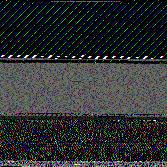
\includegraphics[width=0.3\textwidth]{imgs/proyecto0/boutJPG.jpg}}
&
\subfloat[Imagen en formato PNG]
{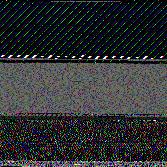
\includegraphics[width=0.3\textwidth]{imgs/proyecto0/boutPNG.png}}
&
\subfloat[Imagen en formato BMP]
{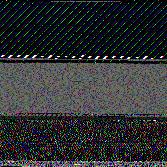
\includegraphics[width=0.3\textwidth]{imgs/proyecto0/boutPNG.png}}
\\
\end{tabular}
\caption{Imágenes obtenidas de un binario .o.}
\label{F:oo}
\end{figure}

%salida del pdf


\begin{figure}[H]
\centering
\begin{tabular}{c c c}
\subfloat[Imagen en formato JPG]
{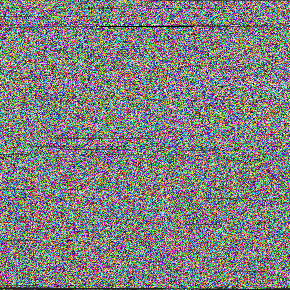
\includegraphics[width=0.3\textwidth]{imgs/proyecto0/outPNG-pdf}}
&
\subfloat[Imagen en formato PNG]
{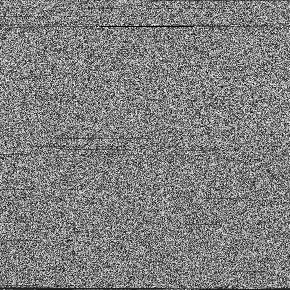
\includegraphics[width=0.3\textwidth]{imgs/proyecto0/outJPG-pdf}}
&
\subfloat[Imagen en formato BMP]
{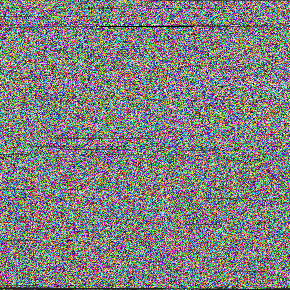
\includegraphics[width=0.3\textwidth]{imgs/proyecto0/outPNG-pdf}}
\\
\end{tabular}
\caption{Imágenes obtenidas de un binario .pdf}
\label{F:pdf}
\end{figure}

\begin{figure}[H]
\centering
\begin{tabular}{c c c}
\subfloat[Imagen en formato JPG]
{\includegraphics[width=0.3\textwidth]{imgs/proyecto0/outPNG-mp3}}
&
\subfloat[Imagen en formato PNG]
{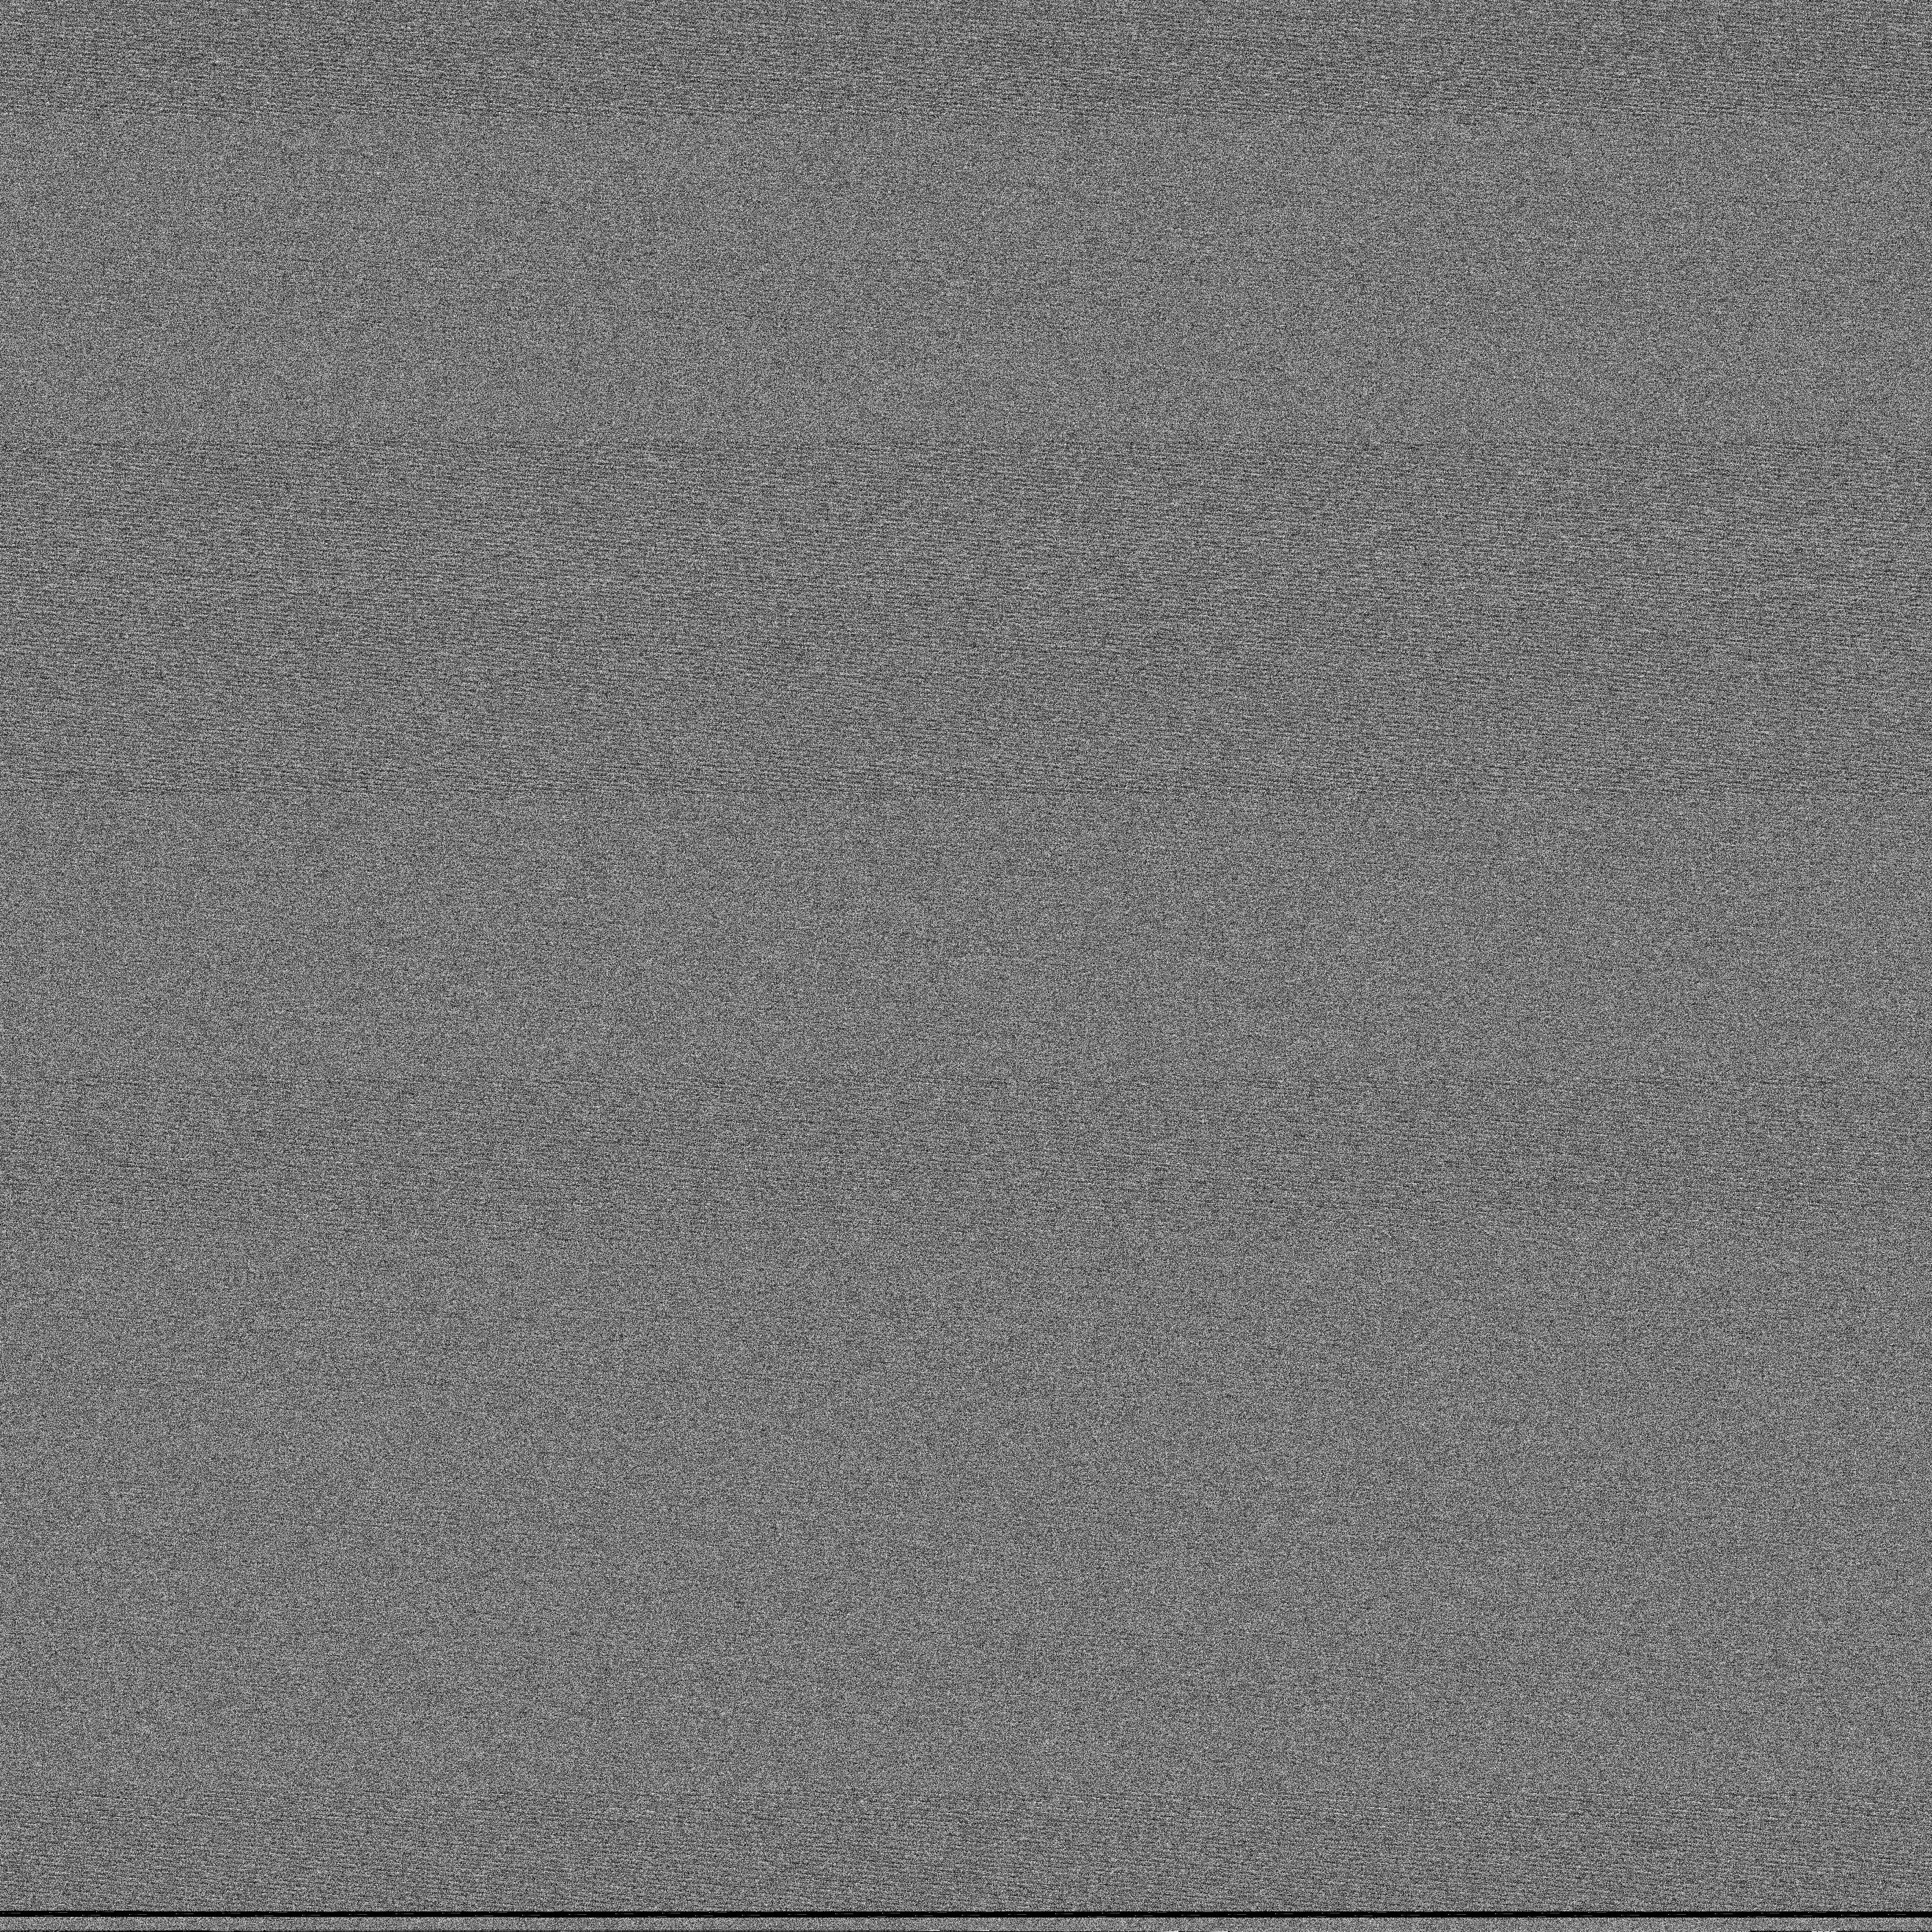
\includegraphics[width=0.3\textwidth]{imgs/proyecto0/outJPG-mp3}}
&
\subfloat[Imagen en formato BMP]
{\includegraphics[width=0.3\textwidth]{imgs/proyecto0/outPNG-mp3}}
\\
\end{tabular}
\caption{Imágenes obtenidas de un binario .mp3}
\label{F:mp3}
\end{figure}

\begin{figure}[H]
\centering
\begin{tabular}{c c c}
\subfloat[Imagen en formato JPG]
{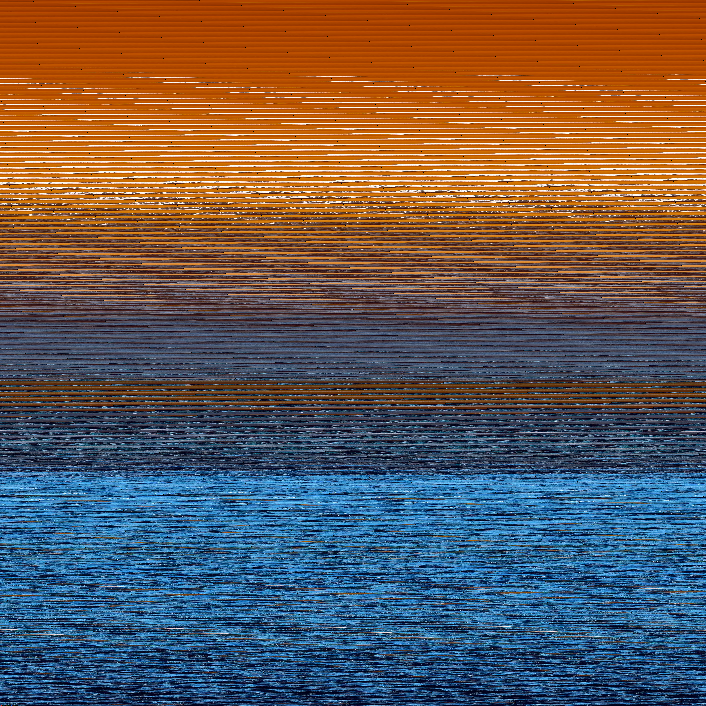
\includegraphics[width=0.3\textwidth]{imgs/proyecto0/outPNG-bmp}}
&
\subfloat[Imagen en formato PNG]
{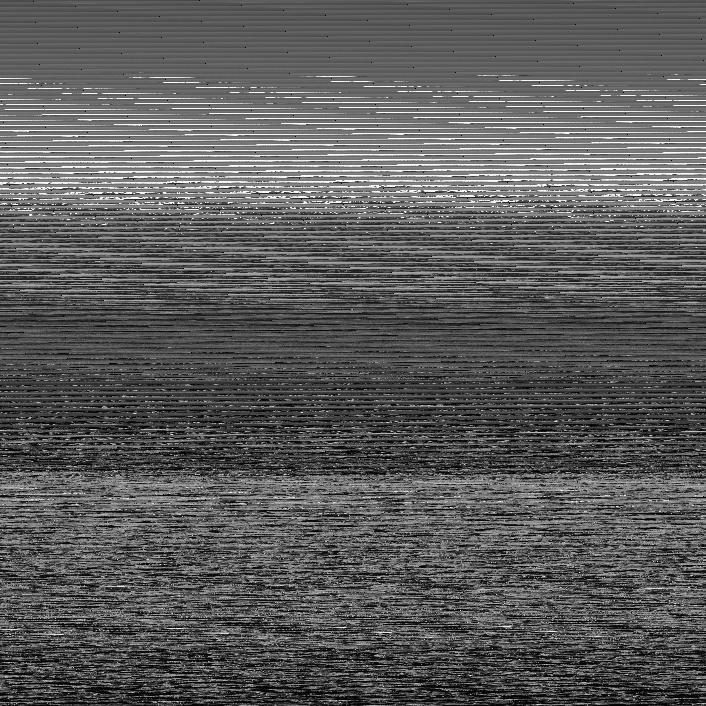
\includegraphics[width=0.3\textwidth]{imgs/proyecto0/outJPG-bmp}}
&
\subfloat[Imagen en formato BMP]
{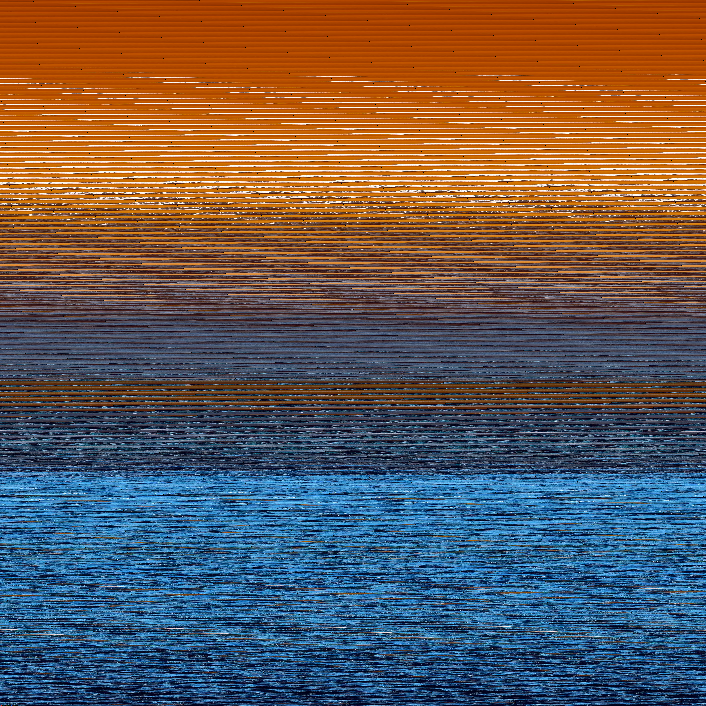
\includegraphics[width=0.3\textwidth]{imgs/proyecto0/outPNG-bmp}}
\\
\end{tabular}
\caption{Imágenes obtenidas de un binario .bmp}
\label{F:bmp}
\end{figure}

%%%%%%%%%%%%%%%%%%%%%%%%%%%%%%%%%%%%%%%%%%%%%%%%%%%%%%%%%%%%%%
% --> ANÁLISIS DE TIEMPOS DE EJECUCIÓN 
%%%%%%%%%%%%%%%%%%%%%%%%%%%%%%%%%%%%%%%%%%%%%%%%%%%%%%%%%%%%%%
\section{Análisis de tiempos de ejecución} 

Al ejecutar el código y crear las imágenes en los distintos formatos se calcula el tiempo de ejecución de cada algoritmo. Se realizaron diez mediciones, y de esta se sacó el promedio que tardó cada función. Se puede notar que la creación de las imágenes en formato BMP y JPEG tienen tiempos muy parecidos, alrededor de 4 segundos. Curiosamente, la creación de la imagen PNG tardó mucho más, un promedio de 21 segundos. La diferencia entre estos tiempos de ejecución está relacionada directamente con la compresión que utiliza cada formato; así como las funciones internas no estudiadas de cada biblioteca utilizada.

\begin{table}[H]
\begin{center}
    \begin{tabular}{ |>{\centering\arraybackslash}m{3cm}|>{\centering\arraybackslash}m{3cm}|>{\centering\arraybackslash}m{3cm}|>{\centering\arraybackslash}m{3cm}| }
    	\hline
    	\cellcolor{cl} \textbf{Tiempo} & \cellcolor{cl} \textbf{BMP} & \cellcolor{cl} \textbf{PNG}  & \cellcolor{cl} \textbf{JPG} \\ \hline \hline
        $T_1$ & 4,38060 & 20,21500 & 4,44193 \\ \hline
        $T_2$ & 4,67325 & 19,40460 & 5,91329 \\ \hline
        $T_3$ & 4,42406 & 24,98370 & 2,36694 \\ \hline
        $T_4$ & 4,34032 & 20,21500 & 2,48694 \\ \hline
        $T_5$ & 4,89789 & 27,75670 & 2,99915 \\ \hline
        $T_6$ & 4,31651 & 19,26920 & 8,54429 \\ \hline
        $T_7$ & 4,22170 & 19,00760 & 1,88674 \\ \hline
        $T_8$ & 4,57719 & 23,82840 & 2,23887 \\ \hline
        $T_9$ & 4,30820 & 21,26630 & 1,95731 \\ \hline
     $T_{10}$ & 4,28089 & 20,12690 & 5,81021 \\ \hline
        \textbf{Prom} & \textbf{4,94206} & \textbf{21,65671 } & \textbf{3,386453} \\ \hline
    \end{tabular}
\end{center}
\label{T:Time}
\caption{Resumen de características de los formatos de imágenes. \cite{R1}}
\end{table}




%%%%%%%%%%%%%%%%%%%%%%%%%%%%%%%%%%%%%%%%%%%%%%%%%%%%%%%%%%%%%%
% --> CONCLUSIONESS 
%%%%%%%%%%%%%%%%%%%%%%%%%%%%%%%%%%%%%%%%%%%%%%%%%%%%%%%%%%%%%%
\section{Conclusiones} 

Como conclusiones se tiene que:
\begin{itemize}
    \item Se logró entender la compresión y el formato de PNG, BMP, JPEG.
    \item Se comprende el modelo de color RGB.
    \item Se logra la lectura en binario permite obtener información en bits y darle cualquier formato para su uso.
     \item Utilización de  bibliotecas de terceros con buena documentación.
    \item Se comprendió cómo se enlazan bibliotecas estáticamente con la creación del programa
\end{itemize}

%%%%%%%%%%%%%%%%%%%%%%%%%%%%%%%%%%%%%%%%%%%%%%%%%%%%%%%%%%%%%%
% --> BIBLIOGRAFIA
%%%%%%%%%%%%%%%%%%%%%%%%%%%%%%%%%%%%%%%%%%%%%%%%%%%%%%%%%%%%%%
\begin{thebibliography}{IEEE}
\bibitem{R1} Luca, M. \textbf{\textit{A Basic Summary of Image Formats}}.  Visto el 5 de Mayo del 2018 en: \url{http://www.student.montefiore.ulg.ac.be/~merciadri/docs/papers/image-formats.pdf}.

\bibitem{R2} Autor Desconocido. \textbf{\textit{Digital images and image formats}}. Visto el 5 de Mayo del 2018 en: \url{http://www.uio.no/studier/emner/matnat/math/MAT-INF1100/h08/kompendiet/images.pdf}.

\bibitem{R3} Brown, A. \textbf{\textit{Graphics File Formats}}. 2008. THe National Archives. Visto el 5 de Mayo del 2018 en: \url{https://www.nationalarchives.gov.uk/documents/graphic-file-formats.pdf}.

\bibitem{R4} PNG. \textit{\textbf{Official documentation of libpng}}. Visto el 5 de Mayo del 2018 en: \url{http://www.libpng.org/pub/png/libpng.html}. 

\bibitem{R5} Kumar, T. Verma, K. \textbf{\textit{A Theory Based on Conversion of RGB image to Gray
image}}. 2010. International Journal of Computer Applications, Vol. 7. No. 2. Visto el 5 de Mayo del 2018 en: \url{https://www.researchgate.net/profile/Karun_Verma/publication/46286639_A_Theory_Based_on_Conversion_of_RGB_image_to_Gray_image/links/5704a3b008ae44d70ee0662c.pdf}.

\bibitem{R6} Greensted, A. \textbf{\textit{Creating PNGs with libpng}}. Visto el 5 de Mayo del 2018 en: \url{http://www.labbookpages.co.uk/software/imgProc/libPNG.html}.

\bibitem{R7} Autor Desconocido. \textbf{\textit{C++ Binary File I/O}}. Visto el 5 de Mayo del 2018 en: \url{http://courses.cs.vt.edu/~cs2604/fall00/binio.html}

\bibitem{R8} Raymon, E. \textbf{\textit{Introduction to GIFLIB}}. Visto el 5 de Mayo del 2018 en: \url{http://giflib.sourceforge.net/intro.html}

\bibitem{R9} Autor desconocido. \textbf{\textit{Magick::Image Class}}. Visto el 5 de Mayo del 2018 en: \url{https://www.imagemagick.org/api/Image++.php}

\end{thebibliography}
-


%%%%%%%%%%%%%%%%%%
%--> LABORATORIO 7
%%%%%%%%%%%%%%%%%%
%%%%%%%%%%%%%%%%%%%%%%%%%%%%%%%%%%%%%%%%%%%%%%%%%%%%%%%%%%%%%%%
% --> INTRODUCCIÓN
%%%%%%%%%%%%%%%%%%%%%%%%%%%%%%%%%%%%%%%%%%%%%%%%%%%%%%%%%%%%%%
\section{Introducción}


%%%%%%%%%%%%%%%%%%%%%%%%%%%%%%%%%%%%%%%%%%%%%%%%%%%%%%%%%%%%%%
% --> OBJETIVOS
%%%%%%%%%%%%%%%%%%%%%%%%%%%%%%%%%%%%%%%%%%%%%%%%%%%%%%%%%%%%%%
\subsection{Objetivos}



%%%%%%%%%%%%%%%%%%%%%%%%%%%%%%%%%%%%%%%%%%%%%%%%%%%%%%%%%%%%%%
% --> OBJETIVO GENERAL
%%%%%%%%%%%%%%%%%%%%%%%%%%%%%%%%%%%%%%%%%%%%%%%%%%%%%%%%%%%%%%
\subsubsection{Objetivo General}
\begin{itemize}
\item 
\end{itemize}

%%%%%%%%%%%%%%%%%%%%%%%%%%%%%%%%%%%%%%%%%%%%%%%%%%%%%%%%%%%%%%
% --> OBJETIVOS ESPECÍFICOS
%%%%%%%%%%%%%%%%%%%%%%%%%%%%%%%%%%%%%%%%%%%%%%%%%%%%%%%%%%%%%%
\subsubsection{Objetivos Específicos}
\begin{itemize}
\item 
\item 
\item 
\item
\item 
\end{itemize}

%%%%%%%%%%%%%%%%%%%%%%%%%%%%%%%%%%%%%%%%%%%%%%%%%%%%%%%%%%%%%%
% --> ENUNCIADO
%%%%%%%%%%%%%%%%%%%%%%%%%%%%%%%%%%%%%%%%%%%%%%%%%%%%%%%%%%%%%%
%\newpage

%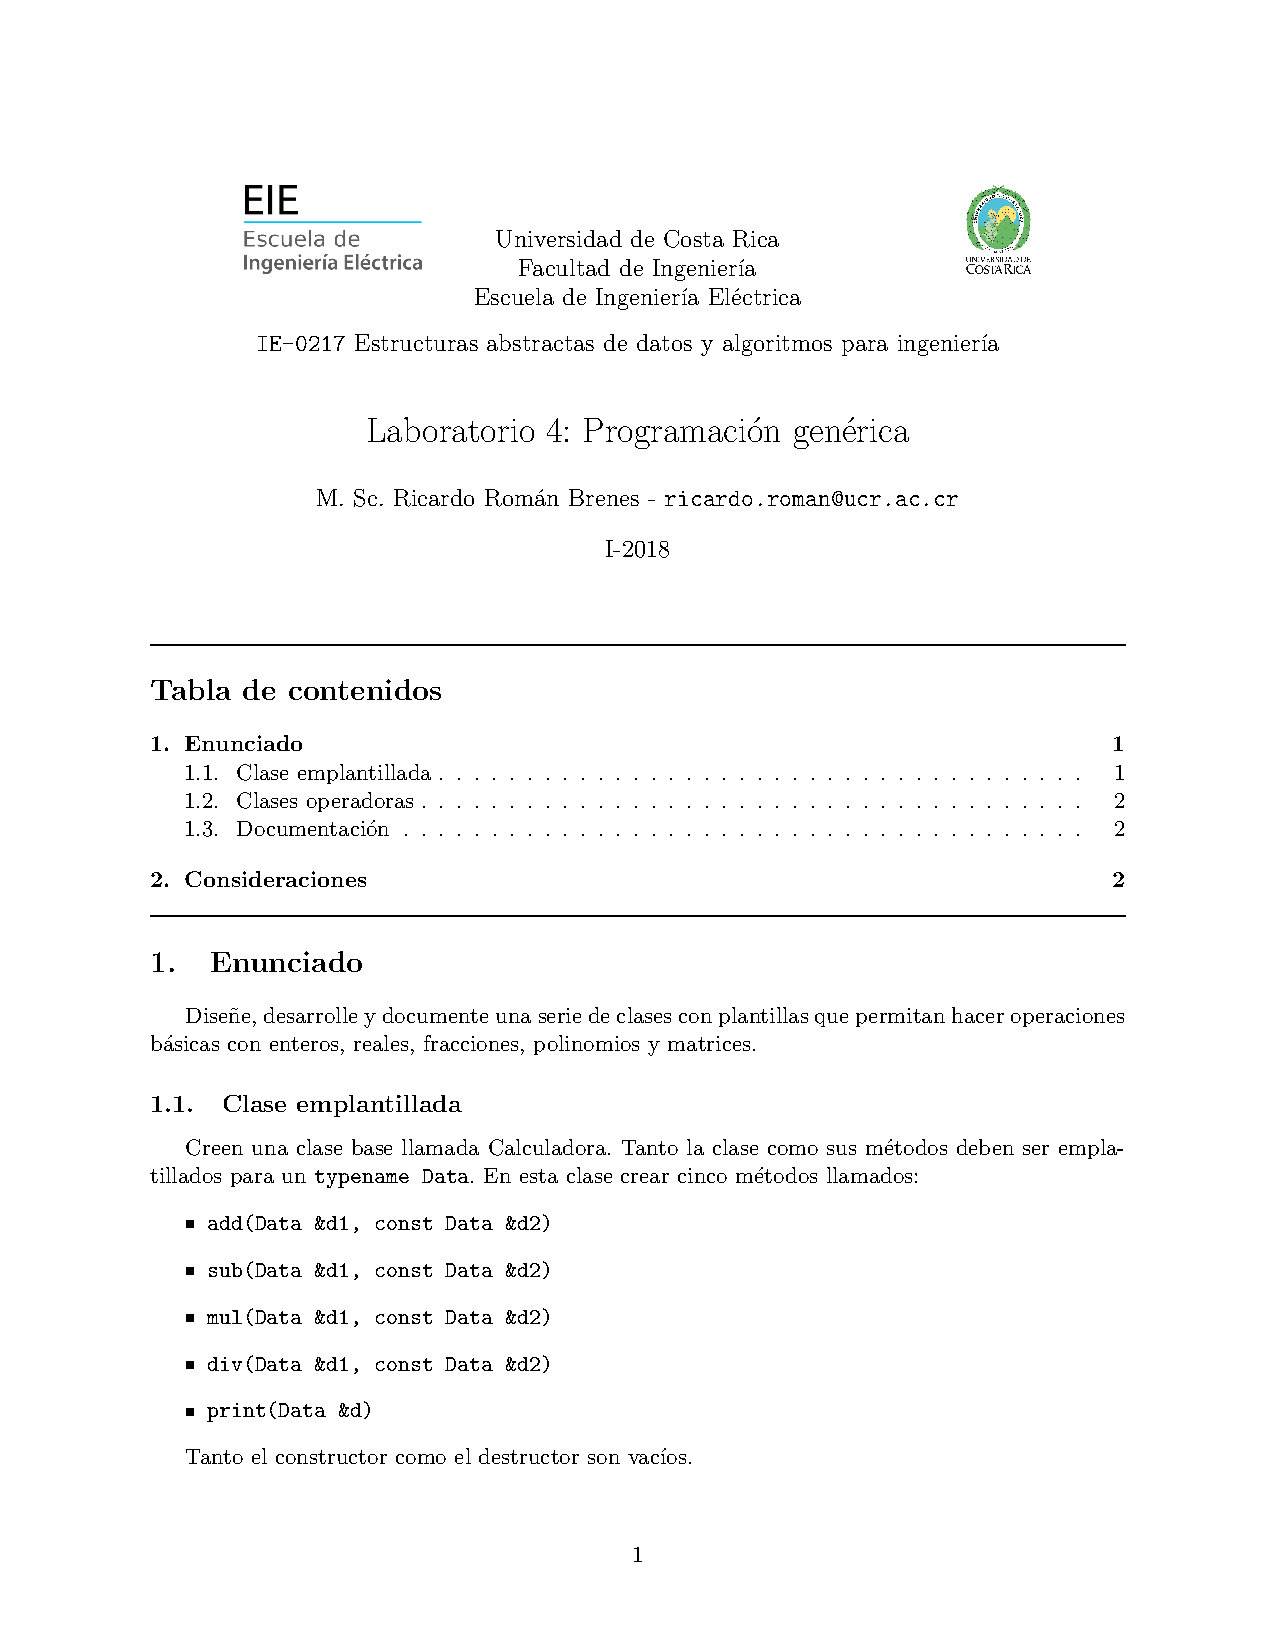
\includepdf[pages=1,pagecommand=\section{Enunciado}, scale=0.8]{enunciados/enun4} 
%\includepdf[pages=2,pagecommand={},scale=0.8]{enunciados/enun4}

%%%%%%%%%%%%%%%%%%%%%%%%%%%%%%%%%%%%%%%%%%%%%%%%%%%%%%%%%%%%%%
% --> SOLUCIÓN
%%%%%%%%%%%%%%%%%%%%%%%%%%%%%%%%%%%%%%%%%%%%%%%%%%%%%%%%%%%%%%
\section{Solución}


\begin{minted}[linenos,autogobble,bgcolor=bg,breaklines,fontsize=\footnotesize ]{c++}
#include <string>
#include <iostream>
using namespace std;

class FileUtil
{
  public:
  	FileUtil(string s, ios_base::openmode p);
  	~FileUtil();
  	string read();
  	string* readLines();
  	int write(string s);
  	int write(string* s, int n);
    void countNumberLines();
    int getNumberLines();
  private:
    //Numero de lineas.
    int numLines;
    //Dirección de lectura.
    string ruta;
    //Modo de lectura.
  	ios_base::openmode modo;
    //Linea leida.
    string line;
    //Puntero con la direccion del arreglo de las lineas leidas.
    string* lines;

};
\end{minted}



%%%%%%%%%%%%%%%%%%%%%%%%%%%%%%%%%%%%%%%%%%%%%%%%%%%%%%%%%%%%%%
% --> RESULTADOS
%%%%%%%%%%%%%%%%%%%%%%%%%%%%%%%%%%%%%%%%%%%%%%%%%%%%%%%%%%%%%%
\section{Resultados}



%%%%%%%%%%%%%%%%%%%%%%%%%%%%%%%%%%%%%%%%%%%%%%%%%%%%%%%%%%%%%%
% --> CONCLUSIONES
%%%%%%%%%%%%%%%%%%%%%%%%%%%%%%%%%%%%%%%%%%%%%%%%%%%%%%%%%%%%%%
\section{Conclusiones}


Como conclusiones se tiene que:

\begin{itemize}
\item 
\item 
\item 
\item 
\end{itemize}


%%%%%%%%%%%%%%%%%%%%%%%%%%%%%%%%%%%%%%%%%%%%%%%%%%%%%%%%%%%%%%
% --> BIBLIOGRAFIA
%%%%%%%%%%%%%%%%%%%%%%%%%%%%%%%%%%%%%%%%%%%%%%%%%%%%%%%%%%%%%%
\begin{thebibliography}{IEEE}
\bibitem{R1} Talens, S. \textbf{\textit{Curso de programación en C++}}. EUI (UPV) Valencia, 17 al 28 de Julio de 1995. 

\bibitem{R2} Raffo, E. \textbf{\textit{Programación genérica en C++, usando Metaprogramación}}. 2007. Sistemas de Informática. 
\end{thebibliography}



%%%%%%%%%%%%%%%%%%
%--> LABORATORIO 8
%%%%%%%%%%%%%%%%%%
%%%%%%%%%%%%%%%%%%%%%%%%%%%%%%%%%%%%%%%%%%%%%%%%%%%%%%%%%%%%%%%
% --> INTRODUCCIÓN
%%%%%%%%%%%%%%%%%%%%%%%%%%%%%%%%%%%%%%%%%%%%%%%%%%%%%%%%%%%%%%
\section{Introducción}


%%%%%%%%%%%%%%%%%%%%%%%%%%%%%%%%%%%%%%%%%%%%%%%%%%%%%%%%%%%%%%
% --> OBJETIVOS
%%%%%%%%%%%%%%%%%%%%%%%%%%%%%%%%%%%%%%%%%%%%%%%%%%%%%%%%%%%%%%
\subsection{Objetivos}



%%%%%%%%%%%%%%%%%%%%%%%%%%%%%%%%%%%%%%%%%%%%%%%%%%%%%%%%%%%%%%
% --> OBJETIVO GENERAL
%%%%%%%%%%%%%%%%%%%%%%%%%%%%%%%%%%%%%%%%%%%%%%%%%%%%%%%%%%%%%%
\subsubsection{Objetivo General}
\begin{itemize}
\item 
\end{itemize}

%%%%%%%%%%%%%%%%%%%%%%%%%%%%%%%%%%%%%%%%%%%%%%%%%%%%%%%%%%%%%%
% --> OBJETIVOS ESPECÍFICOS
%%%%%%%%%%%%%%%%%%%%%%%%%%%%%%%%%%%%%%%%%%%%%%%%%%%%%%%%%%%%%%
\subsubsection{Objetivos Específicos}
\begin{itemize}
\item 
\item 
\item 
\item
\item 
\end{itemize}

%%%%%%%%%%%%%%%%%%%%%%%%%%%%%%%%%%%%%%%%%%%%%%%%%%%%%%%%%%%%%%
% --> ENUNCIADO
%%%%%%%%%%%%%%%%%%%%%%%%%%%%%%%%%%%%%%%%%%%%%%%%%%%%%%%%%%%%%%
%\newpage

%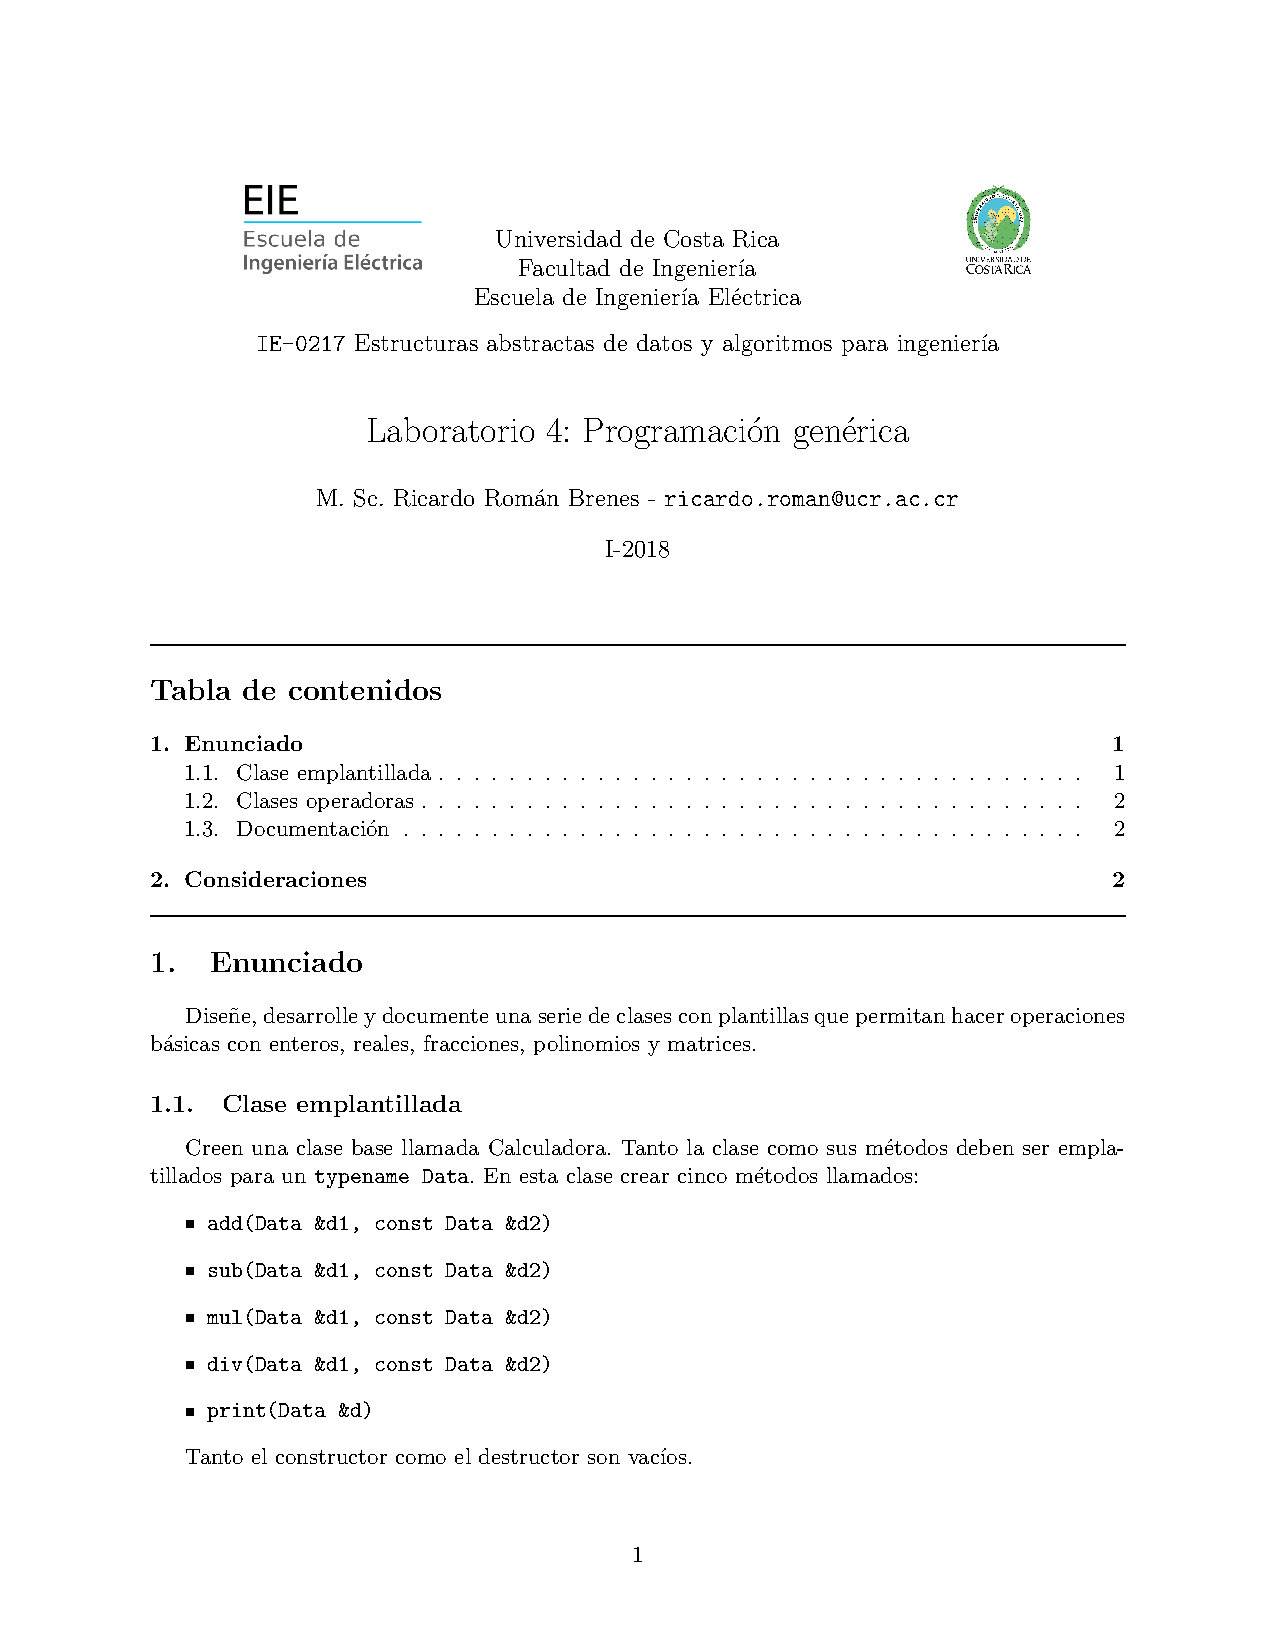
\includepdf[pages=1,pagecommand=\section{Enunciado}, scale=0.8]{enunciados/enun4} 
%\includepdf[pages=2,pagecommand={},scale=0.8]{enunciados/enun4}

%%%%%%%%%%%%%%%%%%%%%%%%%%%%%%%%%%%%%%%%%%%%%%%%%%%%%%%%%%%%%%
% --> SOLUCIÓN
%%%%%%%%%%%%%%%%%%%%%%%%%%%%%%%%%%%%%%%%%%%%%%%%%%%%%%%%%%%%%%
\section{Solución}


\begin{minted}[linenos,autogobble,bgcolor=bg,breaklines,fontsize=\footnotesize ]{c++}
#include <string>
#include <iostream>
using namespace std;

class FileUtil
{
  public:
  	FileUtil(string s, ios_base::openmode p);
  	~FileUtil();
  	string read();
  	string* readLines();
  	int write(string s);
  	int write(string* s, int n);
    void countNumberLines();
    int getNumberLines();
  private:
    //Numero de lineas.
    int numLines;
    //Dirección de lectura.
    string ruta;
    //Modo de lectura.
  	ios_base::openmode modo;
    //Linea leida.
    string line;
    //Puntero con la direccion del arreglo de las lineas leidas.
    string* lines;

};
\end{minted}



%%%%%%%%%%%%%%%%%%%%%%%%%%%%%%%%%%%%%%%%%%%%%%%%%%%%%%%%%%%%%%
% --> RESULTADOS
%%%%%%%%%%%%%%%%%%%%%%%%%%%%%%%%%%%%%%%%%%%%%%%%%%%%%%%%%%%%%%
\section{Resultados}



%%%%%%%%%%%%%%%%%%%%%%%%%%%%%%%%%%%%%%%%%%%%%%%%%%%%%%%%%%%%%%
% --> CONCLUSIONES
%%%%%%%%%%%%%%%%%%%%%%%%%%%%%%%%%%%%%%%%%%%%%%%%%%%%%%%%%%%%%%
\section{Conclusiones}


Como conclusiones se tiene que:

\begin{itemize}
\item 
\item 
\item 
\item 
\end{itemize}


%%%%%%%%%%%%%%%%%%%%%%%%%%%%%%%%%%%%%%%%%%%%%%%%%%%%%%%%%%%%%%
% --> BIBLIOGRAFIA
%%%%%%%%%%%%%%%%%%%%%%%%%%%%%%%%%%%%%%%%%%%%%%%%%%%%%%%%%%%%%%
\begin{thebibliography}{IEEE}
\bibitem{R1} Talens, S. \textbf{\textit{Curso de programación en C++}}. EUI (UPV) Valencia, 17 al 28 de Julio de 1995. 

\bibitem{R2} Raffo, E. \textbf{\textit{Programación genérica en C++, usando Metaprogramación}}. 2007. Sistemas de Informática. 
\end{thebibliography}



%%%%%%%%%%%%%%%%%%
%--> LABORATORIO 9
%%%%%%%%%%%%%%%%%%
%%%%%%%%%%%%%%%%%%%%%%%%%%%%%%%%%%%%%%%%%%%%%%%%%%%%%%%%%%%%%%%
% --> INTRODUCCIÓN
%%%%%%%%%%%%%%%%%%%%%%%%%%%%%%%%%%%%%%%%%%%%%%%%%%%%%%%%%%%%%%
\section{Introducción}

Como se menciona en \cite{R3}, en ciencias de la computación, un árbol binario es una estructura de datos en la cual cada nodo puede tener un hijo izquierdo y un hijo derecho. No pueden tener más de dos hijos (de ahí el nombre "binario"). Si algún hijo tiene como referencia a null, es decir que no almacena ningún dato, entonces este es llamado un nodo externo. En el caso contrario el hijo es llamado un nodo interno. Usos comunes de los árboles binarios son los árboles binarios de búsqueda, los montículos binarios y Codificación de Huffman.

En la figura \ref{fig:tree}, se observa una imagen que ayuda a ejemplificar la estructura básica de un árbol binario.

\begin{figure}[H]
\centering
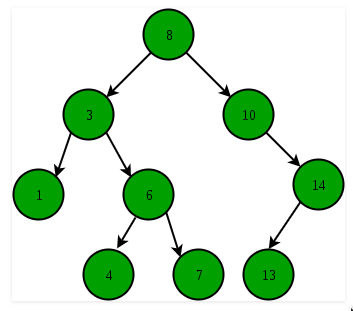
\includegraphics[width=0.45\textwidth]{imgs/Labo9/tree.png}
\caption{Estructura de datos tipo árbol}
\label{fig:tree}
\end{figure}

Un árbol binario es un árbol en el que ningún nodo puede tener más de dos subárboles. En un árbol binario cada nodo puede tener cero, uno o dos hijos (subárboles). Se conoce el nodo de la izquierda como hijo izquierdo y el nodo de la derecha como hijo derecho. Además se debe cumplir que ningún valor del árbol se puede repetir y además, el hijo de la izquierda es menor y el hijo de la derecha es mayor.

Existen tipos de árboles binarios que suelen usarse para fines específicos, como:

\begin{itemize}
    \item Árbol binario de búsqueda
    \item Árbol de Fibonacci
\end{itemize}

También es común hablar de métodos de recorrido de un árbol binario, por lo que más comunes son:

\begin{itemize}
    \item Recorrido en \texttt{preorden}
    \item Recorrido en \texttt{postorden}
    \item Recorrido en \texttt{inorden}
\end{itemize}

Por lo tanto, en este laboratorio se va a trabajar con este tipo de estructura de datos.




%%%%%%%%%%%%%%%%%%%%%%%%%%%%%%%%%%%%%%%%%%%%%%%%%%%%%%%%%%%%%%
% --> OBJETIVOS
%%%%%%%%%%%%%%%%%%%%%%%%%%%%%%%%%%%%%%%%%%%%%%%%%%%%%%%%%%%%%%
\subsection{Objetivos}

%%%%%%%%%%%%%%%%%%%%%%%%%%%%%%%%%%%%%%%%%%%%%%%%%%%%%%%%%%%%%%
% --> OBJETIVO GENERAL
%%%%%%%%%%%%%%%%%%%%%%%%%%%%%%%%%%%%%%%%%%%%%%%%%%%%%%%%%%%%%%
\subsubsection{Objetivo General}
\begin{itemize}
\item Desarrollar una estructura de datos tipo árbol binario. 
\end{itemize}

%%%%%%%%%%%%%%%%%%%%%%%%%%%%%%%%%%%%%%%%%%%%%%%%%%%%%%%%%%%%%%
% --> OBJETIVOS ESPECÍFICOS
%%%%%%%%%%%%%%%%%%%%%%%%%%%%%%%%%%%%%%%%%%%%%%%%%%%%%%%%%%%%%%
\subsubsection{Objetivos Específicos}
\begin{itemize}
\item Realizar las funciones para la insertar y remover nodos de un árbol binario y poder realizar operaciones básicas.
\item Crear algoritmos de recorrido de árboles binarios.
\item Programar el algoritmo de balanceo de un árbol.
\item Validar los códigos desarrollados con una serie de pruebas en el programa principal.
\end{itemize}

%%%%%%%%%%%%%%%%%%%%%%%%%%%%%%%%%%%%%%%%%%%%%%%%%%%%%%%%%%%%%%
% --> ENUNCIADO
%%%%%%%%%%%%%%%%%%%%%%%%%%%%%%%%%%%%%%%%%%%%%%%%%%%%%%%%%%%%%%
%\newpage
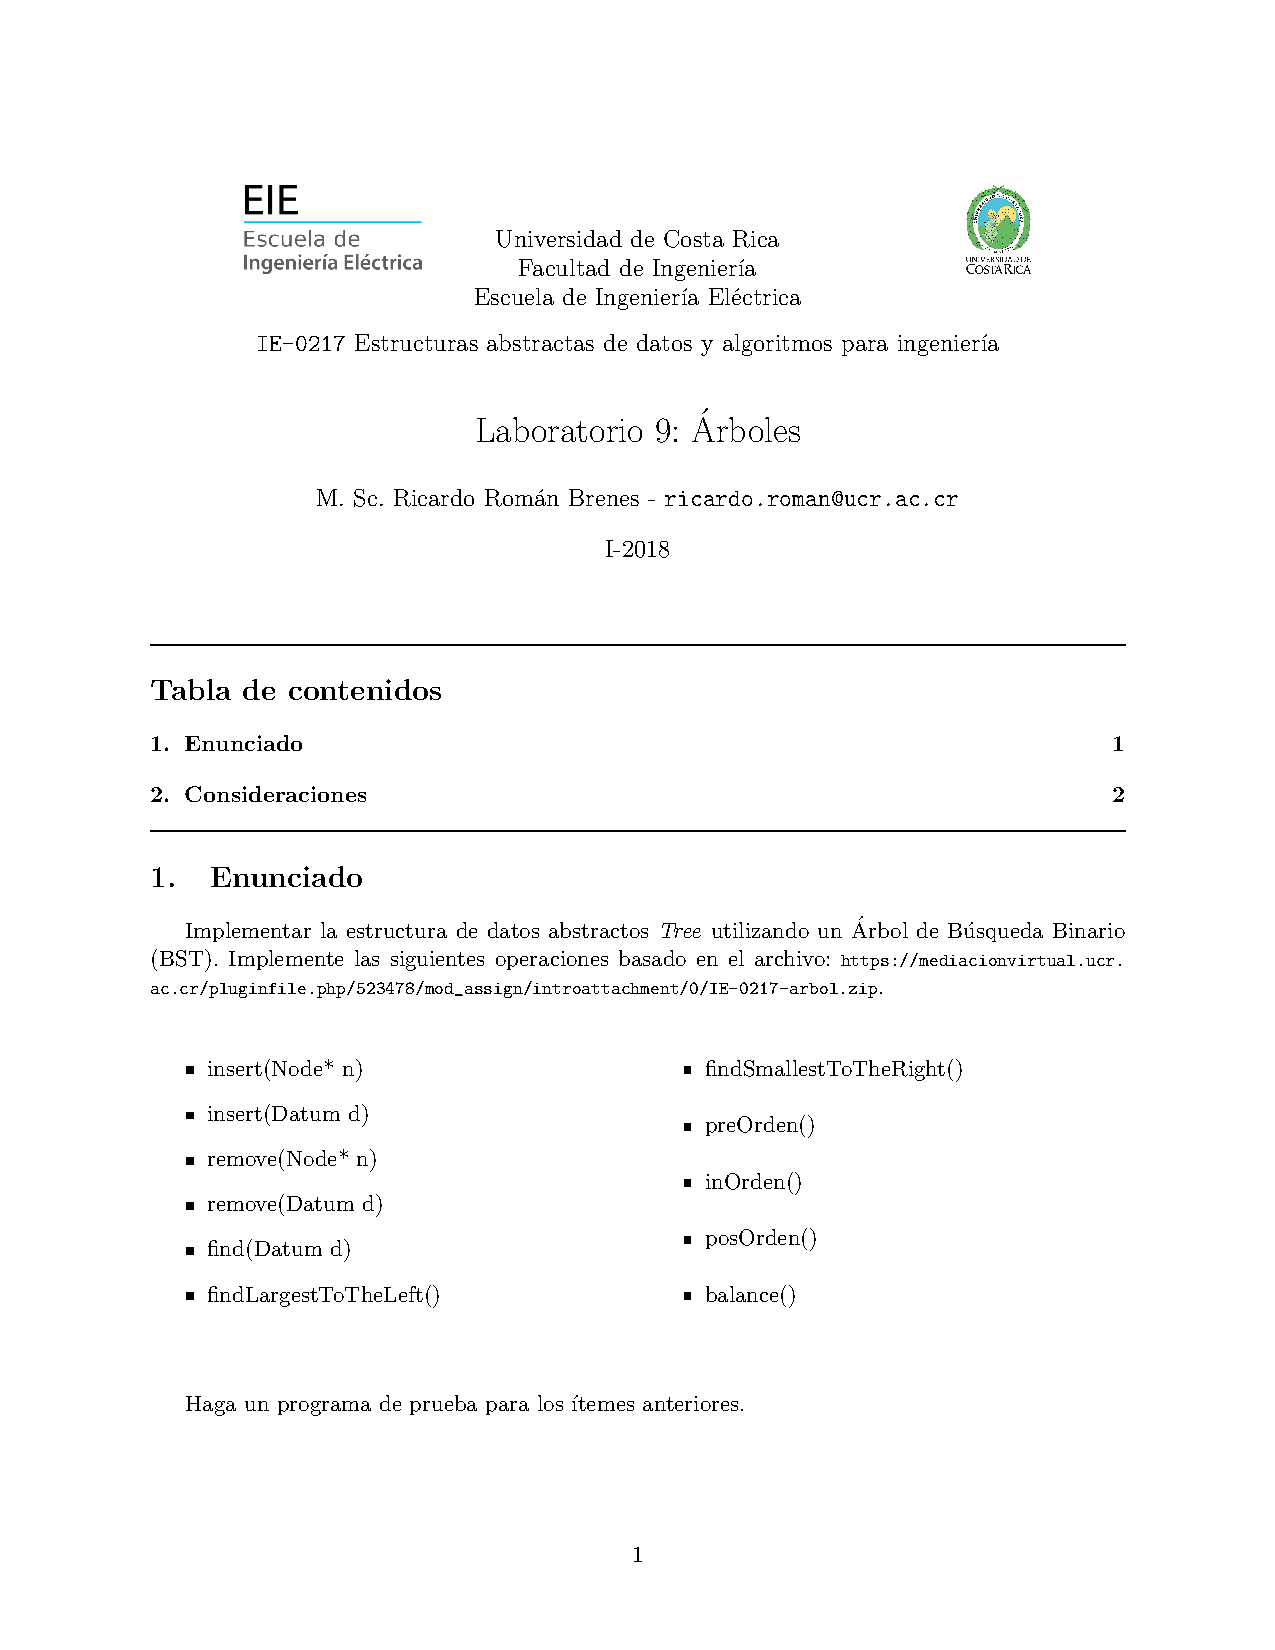
\includepdf[pages=1,pagecommand=\section{Enunciado}, scale=0.8]{enunciados/enun9} 
\includepdf[pages=2,pagecommand={},scale=0.8]{enunciados/enun9}

%%%%%%%%%%%%%%%%%%%%%%%%%%%%%%%%%%%%%%%%%%%%%%%%%%%%%%%%%%%%%%
% --> SOLUCIÓN
%%%%%%%%%%%%%%%%%%%%%%%%%%%%%%%%%%%%%%%%%%%%%%%%%%%%%%%%%%%%%%
\section{Solución}
Para la resolución del laboratorio se utilizaron los archivos proporcionados por el profesor y se procedió a la creación de una serie de métodos para operar sobre el árbol de búsqueda binaria, estos métodos se explican a continuación.
\subsection{Métodos implementados:}

\begin{itemize}
    \item \texttt{insert(Node* n)}: Esta función inserta un nodo \texttt{n} en el árbol, y lo acomoda en la posición adecuada. Para su implementación fue necesario utilizar el método \texttt{iterativeInsert(Node* n)} al que se le agregaron una serie de líneas para almacenar los datos de los hijos derechos e izquierdos.
    
    \begin{minted}[linenos,autogobble,bgcolor=bg,breaklines,fontsize=\footnotesize ]{c++}
    
    void insert(Node* n)
    {
      cout << "Inserting new node "<< n->getDatum() << endl;
      this->nodes++;
      if (!this->root) this->root = n;
      else iterativeInsert(n);
    }
    
    void iterativeInsert(Node* n) 
    {
      bool end = false;
      Node* current = this->root;
      Node* temp;
      while (!end)
      {
        if (!current)
        {
          cout<<"bug:"<< (void*)temp<< endl;
          n->setAncestor(temp);
          current = n;
          end = true;
        } else
        {
          if (current->getDatum() < n->getDatum())
          {
            temp = current;
            current = current->getRightChild();
          }
          else
          {
            temp = current;
            current = current->getLeftChild();
          }
        }
      }
      temp = current->getAncestor();
      if(n->getDatum()<temp->getDatum())
        temp->setLeftChild(n);
      else
        temp->setRightChild(n);
    }
    
    \end{minted}
    
    \item \texttt{remove(Node* n)}: El método \texttt{remove} elimina un nodo del árbol y libera la memoria de los punteros utilizados. Fue necesario implementar otro método que funciona en conjunto llamado \texttt{deleteNode(Node* n, Datum key)} y es llamado desde la función remover.
    
    \begin{minted}[linenos,autogobble,bgcolor=bg,breaklines,fontsize=\footnotesize ]{c++}
    
    void remove(Node* n)
    {
      cout << "Deleting node "<< n->getDatum() << endl;
      this->nodes--;
      this->root = deleteNode(this->root,n->getDatum());
    }
    
    Node* deleteNode(Node* n, Datum key)
    {
      if (key < n->getDatum())
          n->setLeftChild(deleteNode(n->getLeftChild(), key));

      else if (key > n->getDatum())
          n->setRightChild(deleteNode(n->getRightChild(), key));

      else
      {
          if (n->getLeftChild() == NULL)
          {
              Node *temp = n->getRightChild();
              delete n;
              return temp;
          }
          else if (n->getRightChild() == NULL)
          {
              Node *temp = n->getLeftChild();
              delete n;
              return temp;
          }

          Node* temp = findSmallestToTheRight(n);

          n->setDatum(temp->getDatum());

          n->setRightChild(deleteNode(n->getRightChild(), temp->getDatum()));
      }
      return n;
    };
    \end{minted}

    \item \texttt{find(Datum d)}: Este método es el encargado de devolver la dirección en la que se encuentra el dato \texttt{d}, para esto utiliza una función \texttt{search(Node* n, Datum d)} que comprueba si el dato se encuentra en el árbol.
    
    \begin{minted}[linenos,autogobble,bgcolor=bg,breaklines,fontsize=\footnotesize ]{c++}
    
    Node* find(Datum d)
    {
      return search(this->root,d);
    }

    Node* search(Node* n, Datum d)
    {
      if (n == 0x0) {cout<<"Data '"<<d<< "' hasn't been found in the tree"<<endl; return 0x0;}
      else if (n->getDatum() == d) return n;

      if (n->getDatum() < d) return search(n->getRightChild(), d);

      return search(n->getLeftChild(), d);
    }

    Datum find(Node* n)
    {
      return n->getDatum();
    }

    \end{minted}

    \item \texttt{findLargestToTheLeft()}: Como lo dice su nombre, esta función retorna el nodo más grande a la izquierda del árbol.
    
    \begin{minted}[linenos,autogobble,bgcolor=bg,breaklines,fontsize=\footnotesize ]{c++}
    
    Node* findLargestToTheLeft(Node* n)
    {
        Node* s = n->getLeftChild();
        if (s == NULL){
          cout << "No hay elementos a la izquierda" << endl;
          return s;
        }
        while (s->getRightChild()!= NULL)
          s = s->getRightChild();
        return s;
    }
    \end{minted}

    \item \texttt{findSmallestToTheRight()}: Función que regresa el nodo más pequeño a la derecha del árbol.
    
    \begin{minted}[linenos,autogobble,bgcolor=bg,breaklines,fontsize=\footnotesize ]{c++}
    Node* findSmallestToTheRight(Node* n)
    {
      Node* s = n->getRightChild();
      if(s == NULL) {cout << "No hay elementos a la derecha" << endl; return s;}
      while(s->getLeftChild() != NULL)
        s = s->getLeftChild();
      return s;
    }
    \end{minted}
    
    \item \texttt{Funciones de ordenamiento}: Para el ordenamiento de los elementos del árbol se implementaron tres métodos con tres tipos diferentes de ordenamiento. La función \texttt{preOrden()} ordena los elementos del árbol en orden ascendente, mientras que la función \texttt{posOrden()} lo hace al contrario, es decir, descendentemente. La última forma de ordenamiento, \texttt{inOrden()}, es peculiar debido a que coloca primero el valor de la raíz del árbol, seguido por los valores menores, y a continuación todos los valores mayores. Todos estos métodos funcionan recibiendo como parámetro el nodo raíz del árbol.
    
    \begin{minted}[linenos,autogobble,bgcolor=bg,breaklines,fontsize=\footnotesize ]{c++}
    void preOrden(Node * n)
    {
      if (n == NULL) return;
      preOrden(n->getLeftChild());
      cout << n->getDatum() << endl;
      preOrden(n->getRightChild());
    };

    void posOrden(Node * n)
    {
      if (n == NULL ) return;
      posOrden(n->getRightChild());
      cout << n->getDatum() << endl;
      posOrden(n->getLeftChild());
    };

    void inOrden(Node * n)
    {
      if (n == NULL) return;
      cout << n->getDatum() << endl;
      inOrden(n->getLeftChild());
      inOrden(n->getRightChild());
    };

    \end{minted}
    
    \item \texttt{balance()}: Se buscó implementar un método para balancear un árbol binario. Es decir, que dado un árbol que tiene una cantidad mayor de niveles que la necesaria, se modifique de tal forma que se use la menor cantidad de niveles posible y que las ramas estén distribuidas equitativamente. Para lograr esto, se decidió almacenar todos los valores de los nodos del árbol, en orden ascendente (\textit{inOrder}) en una lista enlazada (en este caso, se utilizó la clase \texttt{listWithPointer} anteriormente creada). Luego de esto, se quiso implementar un algoritmo que, partiera la lista a la mitad y tomara este valor medio para insertarlo en el árbol. Haciendo esto recursivamente, se lograría insertar los nodos en el orden óptimo de tal forma que el árbol quedara balanceado. Este último paso no se logró implementar satisfactoriamente.
    
    \begin{minted}[linenos,autogobble,bgcolor=bg,breaklines,fontsize=\footnotesize ]{c++}
    void balancear()
    {
	    if (this->getRootNode() == NULL) cout << "No se puede balancear arbol vacío" << endl;
		fillArray(this->root);
		//vaciar el árbol
		cout << "destruyendo" << endl;
		DestroyRecursive(this->root);
		//reconstruir árbol a partir de elementos de la lista
		ListToBST(this->list->getFirst(),0,this->list->getSize()-1);
    // };
    
    //funcion para pasar elementos del arbol a una lista enlazada
    void fillArray(Node * n) // l d r
    {
    if (n == NULL) return;
    fillArray(n->getLeftChild());
    this->list->insert(n->getDatum());
    fillArray(n->getRightChild());
    };
    
    void ListToBST(SimpleNode<Datum>* element, int start, int end){
		if (start>end) return;
		int mid = start + (end-start)/2;
		cout << "mid: " << mid << endl;
		Node* leftChild = listToBST(element,start,mid-1);
		cout << "created lc" << endl;
		cout << "element value: " << element->value << endl;
		Node* parent = new Node(element->value);
		cout << "created node" << endl;		parent->setLeftChild(leftChild);
		element=element->getNext();
		parent->setRightChild(listToBST(element,mid,end));
		this->insert(parent);
	};
    \end{minted}
    
\end{itemize}


%%%%%%%%%%%%%%%%%%%%%%%%%%%%%%%%%%%%%%%%%%%%%%%%%%%%%%%%%%%%%%
% --> RESULTADOS
%%%%%%%%%%%%%%%%%%%%%%%%%%%%%%%%%%%%%%%%%%%%%%%%%%%%%%%%%%%%%%
\section{Resultados}

En las siguientes figuras se observan los resultados al ejecutar las funciones creadas, para esto se utilizó el código escrito en el \texttt{main}, que se adjunta a continuación. En la Figura \ref{fig:1} se observa la creación de un árbol y además se observa que se le añaden nodos con diversos valores. EN la parte inferior se puede observar el resultado de imprimir el árbol, donde se nota la correspondencia de los punteros de los nodos, lo que nos indica que estos están correctamente enlazados, este árbol tiene una estructura como la que se observa entre las líneas 13 y 20 del código.


    
    \begin{minted}[linenos,autogobble,bgcolor=bg,breaklines,fontsize=\footnotesize ]{c++}
    #include <iostream>
    #include "../include/BST.hpp"
    #include "../include/BSTNode.hpp"
    using namespace std;
    
    int main(int argc, char** argv)
    {
        //Se crea un árbol binario
        BST< BSTNode<int>,int >* littleTree = new BST< BSTNode<int>,int >();
        //Se crean nodos para el árbol
        BSTNode<int>* _50 = new BSTNode<int>(0x0, 0x0, 50);
        BSTNode<int>* _25 = new BSTNode<int>(0x0, 0x0, 25);
        BSTNode<int>* _75 = new BSTNode<int>(0x0, 0x0, 75);
        BSTNode<int>* _10 = new BSTNode<int>(0x0, 0x0, 10);
        BSTNode<int>* _420 = new BSTNode<int>(0x0, 0x0, 420);
        BSTNode<int>* _60 = new BSTNode<int>(0x0, 0x0, 60);
        BSTNode<int>* _40 = new BSTNode<int>(0x0, 0x0, 40);
        BSTNode<int>* _15 = new BSTNode<int>(0x0, 0x0, 15);
        /* Insertando los nodos al árbol, para que quede de la siguiente manera:
        *                    50
        *                  /    \
        *                25     75
        *               /  \   /  \
        *             10  40  60  420
        *               \
        *               15
        */
        littleTree->insert(_50);
        littleTree->insert(_25);
        littleTree->insert(_75);
        littleTree->insert(_10);
        littleTree->insert(_420);
        littleTree->insert(_60);
        littleTree->insert(_40);
        littleTree->insert(_15);
        // Imprimiendo árbol manualmente nodo por nodo
        cout <<endl<<separator<<"Printing resulting tree" <<endl<<endl;
        _50->printMe();
        _25->printMe();
        _10->printMe();
        _75->printMe();
        _420->printMe();
        _60->printMe();
        _40->printMe();
        _15->printMe();
    \end{minted}



\begin{figure}[H]
\centering
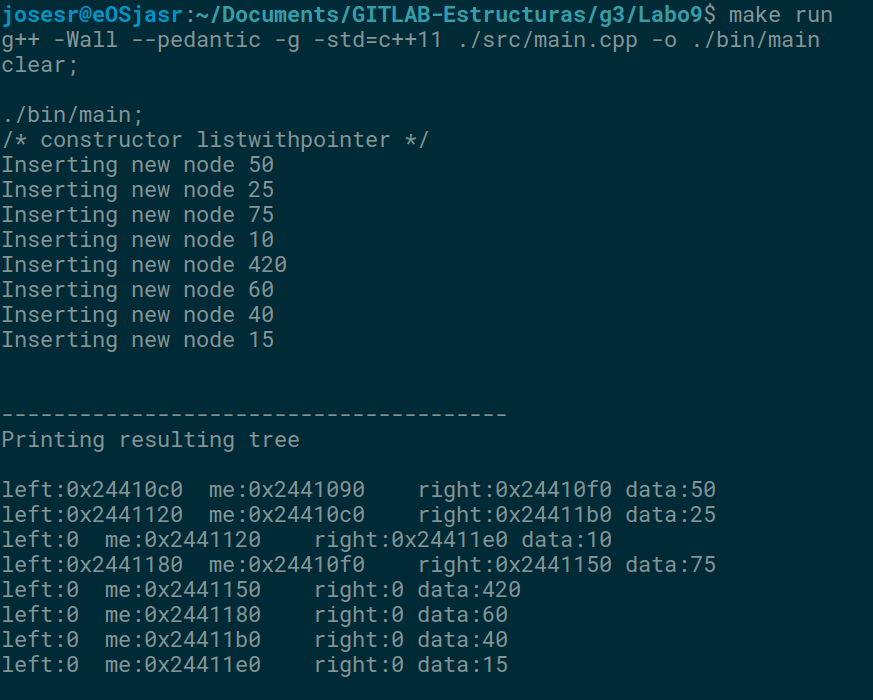
\includegraphics[width=\textwidth]{imgs/Labo9/L9-1.png}
\caption{Creación del árbol, inserción de nodos e impresión del árbol.}
\label{fig:1}
\end{figure}

En la Figura \ref{fig:2} se puede observar las pruebas realizadas para el despliegue de ciertos datos de interés, por ejemplo, podemos observar la raíz del árbol que se creó anteriormente, así como el valor que este nodo almacena. También se probaron las funciones \texttt{findLargestToTheLeft} y \texttt{findSmallestToTheRight}, que devolvieron los valores esperados. Además se comprobó el correcto funcionamiento de las funciones de búsqueda \texttt{find}.

\begin{minted}[linenos,autogobble,bgcolor=bg,breaklines,fontsize=\footnotesize ]{c++}
    const char * separator = "\n---------------------------------------\n"
    cout <<endl<<separator<<"----------- Algunas pruebas ----------- " << endl<<endl;
    BSTNode<int>* littleRoot = littleTree->getRootNode();
    cout << "Root del árbol: " << littleRoot << endl;
    cout << "Valor almacenado en el root: " << littleTree->getRootValue() << endl;
    BSTNode<int>* test = new BSTNode<int>(0);
    cout <<separator<< "Probando findLargestToTheLeft: " << endl;
    test = littleTree->findLargestToTheLeft(littleRoot);
    test->printMe();
    cout << endl << "Probando findSmallestToTheRight: " << endl;
    test = littleTree->findSmallestToTheRight(littleRoot);
    test->printMe();
    cout <<separator<< "Probando find(-2) (dato que no existe): " << endl;
    test = littleTree->find(-2);
    test->printMe();
    cout << endl << "Probando find(root): " << endl;
    cout << littleTree->find(littleRoot) << endl;
    cout << endl <<  "Probando find(root->leftChild): " << endl;
    cout << littleTree->find(littleRoot->getLeftChild()) << endl;
    cout << endl << "Probando find(root->rightChild): " << endl;
    cout << littleTree->find(littleRoot->getRightChild()) << endl;
\end{minted}

\begin{figure}[H]
\centering
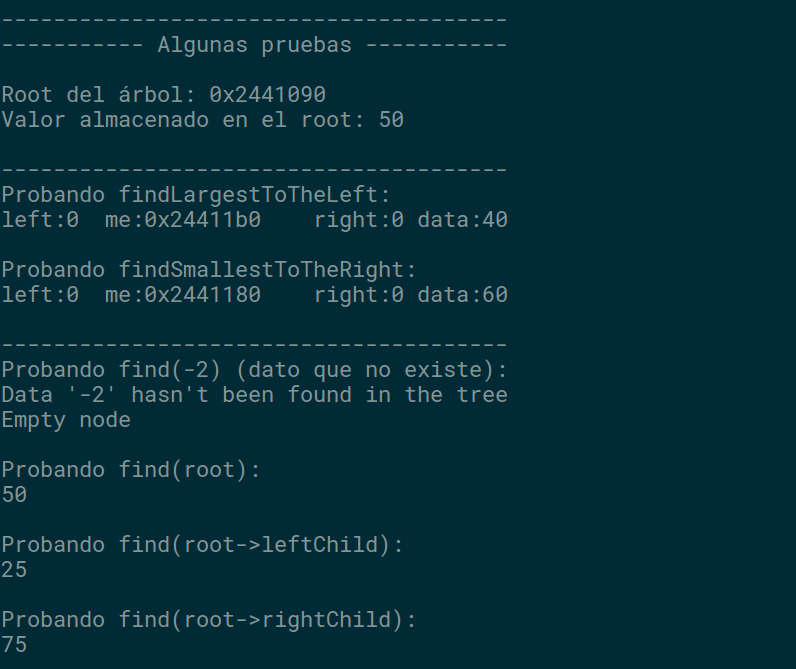
\includegraphics[width=0.85\textwidth]{imgs/Labo9/L9-2.png}
\caption{Prueba de métodos de búsqueda.}
\label{fig:2}
\end{figure}



\begin{minted}[linenos,autogobble,bgcolor=bg,breaklines,fontsize=\footnotesize ]{c++}
    cout <<separator<<"Imprimiendo preOrden " << endl<<endl;
    littleTree->preOrden(littleRoot);
    cout <<separator<<"Imprimiendo  inOrden " << endl<<endl;
    littleTree->inOrden(littleRoot);
    cout <<separator<<"Imprimiendo  posOrden " << endl<<endl;
    littleTree->posOrden(littleRoot);
    \end{minted}

Al aplicar los tres tipos de ordenamiento se obtiene el resultado de la Figura \ref{fig:3}, donde se observa que son resultados satisfactorios.

\begin{figure}[H]
\centering
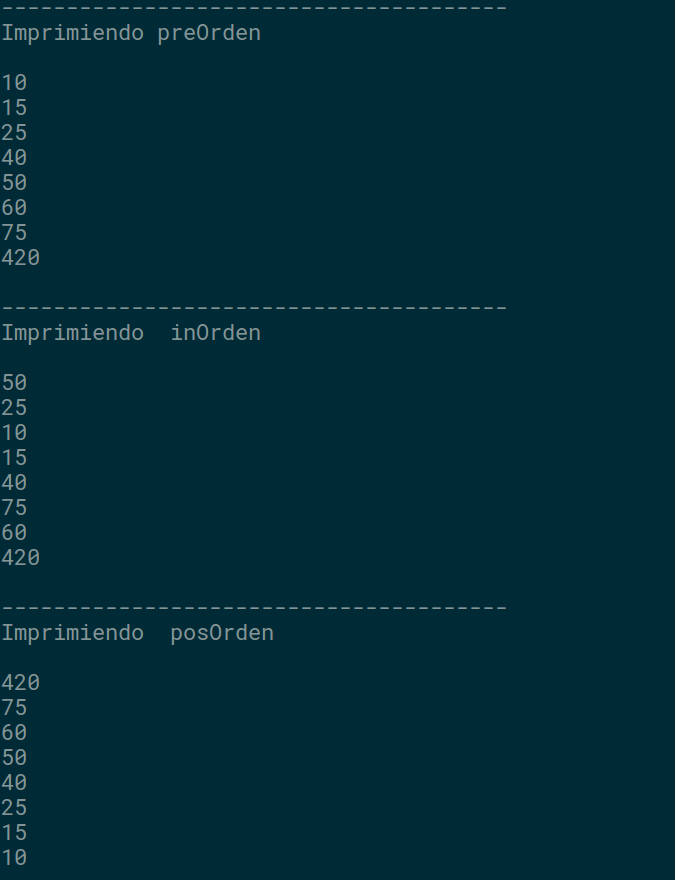
\includegraphics[width=0.8\textwidth]{imgs/Labo9/L9-3.png}
\caption{Impresión de los métodos de ordenamiento.}
\label{fig:3}
\end{figure}


\begin{minted}[linenos,autogobble,bgcolor=bg,breaklines,fontsize=\footnotesize ]{c++}
    cout <<separator<<"Cantidad de niveles:" << endl<<endl;
    cout << littleTree->getLevels() << endl;
    cout << separator << "Borrando el nodo 50" << endl;
    littleTree->remove(_50);
    cout << "Nuevo root del árbol: " << littleTree->getRootNode() << endl;
    cout << "Valor del nuevo root: " << littleTree->getRootValue() << endl;
    littleRoot = littleTree->getRootNode();
    /*                  60
    *                  /  \
    *                 25  75
    *                /  \   \
    *               10  40  420
    *                 \
    *                 15
    */
    cout << separator << "Llenar lista con valores almacenados, en orden ascendente: " << endl;
    littleTree->fillArray(littleRoot);
    littleTree->printList();
    cout <<endl<<"test----- " << endl<<endl
    littleTree->remove(_40);
    cout << "Root value: " << littleTree->getRootValue() << endl;
    \end{minted}

En la Figura \ref{fig:4} se imprimió la cantidad de niveles del árbol obtenida con el método creado y ya comentado. También se probó la eliminación del nodo raíz del árbol y seguidamente la asignación de una nueva raíz. Con el método \texttt{fillArray} se creó una lista enlazada que contiene los valores del árbol ordenados de forma ascendente.

\begin{figure}[H]
\centering
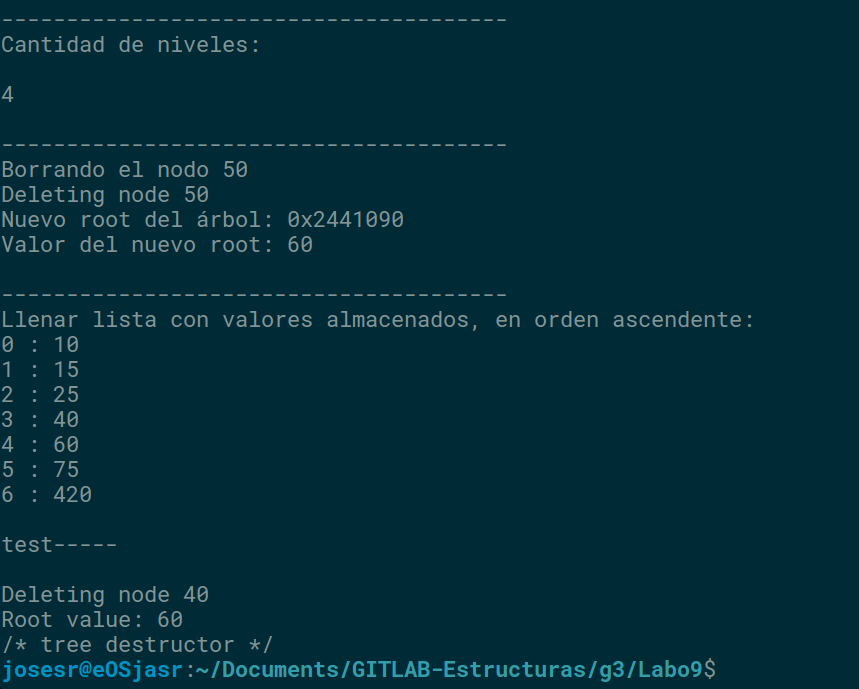
\includegraphics[width=0.9\textwidth]{imgs/Labo9/L9-4.png}
\caption{Creación de una lista con los valores ordenados del árbol.}
\label{fig:4}
\end{figure}


%%%%%%%%%%%%%%%%%%%%%%%%%%%%%%%%%%%%%%%%%%%%%%%%%%%%%%%%%%%%%%
% --> CONCLUSIONES
%%%%%%%%%%%%%%%%%%%%%%%%%%%%%%%%%%%%%%%%%%%%%%%%%%%%%%%%%%%%%%
\section{Conclusiones}


Como conclusiones se tiene que:

\begin{itemize}
\item Se implementó correctamente una estructura de datos de tipo árbol binario.
\item Se logró  implementar correctamente las funciones para insertar y remover nodos en un árbol binario.
\item Se crearon correctamente los métodos necesarios para recorrer los árboles, así como para ordenar sus elementos.
\item La creación del método de balanceo del árbol resultó satisfactoria y eficaz.
\item Se comprobó el funcionamiento de todos los métodos con una serie de pruebas desplegadas en la terminal.
\end{itemize}


%%%%%%%%%%%%%%%%%%%%%%%%%%%%%%%%%%%%%%%%%%%%%%%%%%%%%%%%%%%%%%
% --> BIBLIOGRAFIA
%%%%%%%%%%%%%%%%%%%%%%%%%%%%%%%%%%%%%%%%%%%%%%%%%%%%%%%%%%%%%%
\begin{thebibliography}{IEEE}
\bibitem{R1} Talens, S. \textbf{\textit{Curso de programación en C++}}. EUI (UPV) Valencia, 17 al 28 de Julio de 1995. 

\bibitem{R2} Raffo, E. \textbf{\textit{Programación genérica en C++, usando Metaprogramación}}. 2007. Sistemas de Informática. 

\bibitem{R3} Wikipedia \textbf{\textit{Árbol Binario}}. Tomado el 20 de Junio del 2018 en: \url{https://es.wikipedia.org/wiki/\%C3\%81rbol_binario}.

\end{thebibliography}

%%%%%%%%%%%%%%%%%%
%--> PROPUESTA PROYECTO 1
%%%%%%%%%%%%%%%%%%
%\newpage
%%%%%%%%%%%%%%%%%%%%%%%%%%%%%%%%%%%%%%%%%%%%%%%%%%%%%%%%%%%%%%%
% --> INTRODUCCIÓN
%%%%%%%%%%%%%%%%%%%%%%%%%%%%%%%%%%%%%%%%%%%%%%%%%%%%%%%%%%%%%%


\section{Enunciado}

El objetivo de este proyecto es familiarizar al estudiante con la programación forma de una
estructura de datos y/o algoritmos clásicos utilizando C++, así como  su análisis y presentación.
En particular este en este proyecto cada grupo deberá realizar el una implementación del tema
seleccionado:

\begin{itemize}
    \item Problema de optimización: método exhaustivo vs. método heurístico(programación genética).
\end{itemize}

En cada caso se debe comparar las dos opciones y verificar tiempos de duración, funciones de duración
y complejidades temporales para diferentes tamaños de N. Recuerde utilizar gráficas y tablas para
sus datos y discutir los resultados.


%%%%%%%%%%%%%%%%%%%%%%%%%%%%%%%%%%%%%%%%%%%%%%%%%%%%%%%%%%%%%%
% --> RESEÑA DEL ALGORITMO/ESTRUCTURA
%%%%%%%%%%%%%%%%%%%%%%%%%%%%%%%%%%%%%%%%%%%%%%%%%%%%%%%%%%%%%%
\section{Reseña del algoritmo/estructura}

Los problemas de optimización consisten en la búsqueda de una solución a un problema, que optimice (maximice o minimice) el resultado en términos de una o más variables de ese problema. Usualmente contiene un espacio de posibles soluciones $X$, y una función $f$ que evalúa las posibles soluciones. Existe gran cantidad de enfoques en los métodos de optimización, algunas que utilizan técnicas basadas en el cálculo, búsquedas aleatorias o técnicas enumerativas \cite{R11}. 

En este proyecto se analizarán dos enfoques específicos de algoritmos de optimización: los métodos exhaustivos y los algoritmos de programación genética. Ambos son métodos de tipo meta-heurístico, lo cual significa que son métodos que no dependen del problema específico a resolver; no tienen una prueba matemática rigurosa pero obtienen la solución buscada en todos los casos prácticos \cite{R11}. A continuación se explica brevemente el concepto detrás de estos tipos de algoritmos, y el problema que se utilizará para compararlos.

\subsection{Método Exhaustivo}
Los algoritmos exhaustivos son algoritmos que exploran todas las combinaciones posibles de elementos con el fin de encontrar la solución a un problema, por esto, también se les conoce como algoritmos de fuerza bruta \cite{R10}. A partir de un espacio de posibles soluciones, enumeran y evalúan cada una de estas para determinar si es la solución buscada para el problema. Estos algoritmos poseen la gran ventaja de ser capaces de encontrar la solución correcta de un problema determinado, no una aproximación; esto con una gran desventaja: su tiempo de ejecución aumenta de gran manera de acuerdo a la magnitud del problema. 


A este tipo de algoritmos se les puede realizar modificaciones de acuerdo a lo que se desee como solución. En algunas situaciones se requiere obtener todo el conjunto de posibles soluciones, por lo que es necesario recorrer todas las posibilidades y almacenar las soluciones. También, se puede presentar la situación en que se busque la solución óptima, en donde de igual manera se debe recorrer todas las posibles soluciones y evaluar para reconocer cuál es la mejor opción.   

\subsection{Método Heurístico (Programación Genética)}

 La programación genética, es un tipo de programación perteneciente al grupo de los Algoritmos Genéticos. Estos algoritmos están basados en el proceso genético de los organismos vivos, establecido en la biología. A partir de una "población inicial" dada, se presentan una serie de eventos de selección, evaluación, mutación y cruce de individuos, dando paso a diferentes \emph{generaciones}. Conforme pasan las generaciones, en la naturaleza las poblaciones evolucionan de acuerdo con los principios de la Selección Natural y la supervivencia de los más fuertes. Esta es la idea detrás de los Algoritmos Genéticos, que básicamente, son algoritmos capaces de evolucionar, o mejorarse a sí mismos a partir de una solución propuesta de forma aleatoria, hasta encontrar la solución al problema, imitando la forma biológica de la Selección Natural. En este tipo de algoritmos se utilizan términos biológicos como ``población'', ``codones'', ``cromosomas'', para detallar el funcionamiento del algoritmo\cite{R12}.


%%%%%%%%%%%%%%%%%%%%%%%%%%%%%%%%%%%%%%%%%%%%%%%%%%%%%%%%%%%%%%
% --> FUNCIONAMIENTO DEL ALGORITMO
%%%%%%%%%%%%%%%%%%%%%%%%%%%%%%%%%%%%%%%%%%%%%%%%%%%%%%%%%%%%%%

\section{Funcionamiento del algoritmo/estructura}

\subsection{Método Exhaustivo}

El funcionamiento básico de este tipo de algoritmos consiste en probar o generar un elemento $c_0$  que puede ser solución de cierto problema $P$. Si se cumple que este elemento $c_0$ es solución, se termina el programa, pero si no es solución, se repite el procedimiento con un elemento $c_1$ y así continuamente hasta agotar el conjunto de posibles soluciones, es decir, hasta el elemento $c_n$, asumiendo que este conjunto es finito y de dimensión $n$. Como se mencionó anteriormente, la desventaja se presenta por que en el peor de los casos la solución es el último elemento o simplemente no existe, por lo que el algoritmo debe recorrer toda la magnitud $n$ del problema; si $n\rightarrow \infty$, tardaría un tiempo infinito, lo anterior no se puede presentar en informática, pero nos indica que tardaría mucho tiempo en realizarse. 

\begin{table}[H]
\centering
\caption{Pseudocódigo del algoritmo de fuerza bruta.}
\label{T:exh}
\begin{tabular}{l}
    \hline
   \cellcolor{lightgray} \textbf{Algoritmo}. Búsqueda por fuerza bruta \\
    \hline
    \hline
     
     $\cdot$ \textbf{Begin}:\\
     \hspace{0.6cm} $\cdot$ c $\leftarrow$ Primero(P)\\
     \hspace{0.6cm} $\cdot$ \textbf{While not} c = NULL \textbf{do}:\\
     \hspace{1.2cm} $\cdot$ \textbf{If} tamaño Valido(P,c) \textbf{do}:\\
     \hspace{1.8cm} Mostrar(P,c) \\\hspace{1.2cm}  $\cdot$  c $\leftarrow$ Siguiente(P,c)\\
     \hspace{0.6cm} $\cdot$ \textbf{End}\\
     $\cdot$ \textbf{End}\\
    \hline
\end{tabular}
\end{table}


\subsection{Método Heurístico (Programación Genética)}
 De forma más detallada, estos algoritmos trabajan con una población o conjunto de individuos que representan posibles soluciones al problema tratado. A estas posibles soluciones se les asigna un valor con el cual se va a trabajar, entre más grande sea la adaptación de esta solución al problema, mayor es la probabilidad de que esta solución sea seleccionada para "reproducirse", y así "cruza" su material genético con otro individuo o solución seleccionada de la misma forma. Esta reproducción generará nuevos individuos (soluciones), también llamados descendientes, los cuales poseen ciertas características "heredadas" de sus "padres"\cite{R12}. 

Una parte primordial del funcionamiento del algoritmo es una función que modela la adaptación del individuo, es decir, al evaluar la solución en ella, nos indica que tan buena o apta es esta solución.  Cuanto menor sea la adaptación de un individuo, menor es la probabilidad de que dicha solución
sea seleccionado para la reproducción, y por tanto de que su "material genético" se herede en sucesivas
generaciones.
\begin{table}[H]
\centering
\caption{Pseudocódigo del algoritmo genético.}
\label{T:gen}
\begin{tabular}{l}
    \hline
   \cellcolor{lightgray} \textbf{Algoritmo}. Optimización genética \\
    \hline
    \hline
     $\cdot$ \textbf{Begin}:\\
     \hspace{0.6cm} $\cdot$ Generar una población inicial.\\
     \hspace{0.6cm} $\cdot$ Computar la función de evaluación de cada individuo.\\
     \hspace{0.6cm} $\cdot$ \textbf{While not} terminado \textbf{do}:\\
     \hspace{0.6cm} $\cdot$ \textbf{Begin}:\\
     \hspace{1.2cm} $\cdot$ \textbf{For} tamaño población \textbf{do}:\\
     \hspace{1.2cm} $\cdot$ \textbf{Begin}:\\
     \hspace{1.8cm} $\Rightarrow$ \texttt{Seleccionar} dos individuos de la anterior generación, para el cruce\\\hspace{1.8cm} (probabilidad de selección proporcional a la función de evaluación del individuo).\\
     \hspace{1.8cm} $\Rightarrow$ \texttt{Cruzar} con cierta probabilidad los dos individuos  obteniendo dos \\\hspace{1.8cm} descendientes. \\
     \hspace{1.8cm} $\Rightarrow$ \texttt{Mutar} los dos descendientes con cierta probabilidad. \\
     \hspace{1.8cm} $\Rightarrow$ \texttt{Computar} la función de evaluación de los dos descendientes mutados.\\
     \hspace{1.8cm} $\Rightarrow$ \texttt{Insertar} los dos descendientes mutados en la nueva generación.\\
     \hspace{1.2cm} $\cdot$ \textbf{End}\\
     \hspace{1.2cm} $\cdot$ \textbf{If}  la población ha convergido \textbf{then}\\
     \hspace{1.2cm} $\cdot$ Terminado = \textbf{True}\\
     \hspace{0.6cm} $\cdot$ \textbf{End}\\
     $\cdot$ \textbf{End}\\
     
    \hline
\end{tabular}
\end{table}

%%%%%%%%%%%%%%%%%%%%%%%%%%%%%%%%%%%%%%%%%%%%%%%%%%%%%%%%%%%%%%
% --> EXPERIMENTOS QUE SE REALIZARAN
%%%%%%%%%%%%%%%%%%%%%%%%%%%%%%%%%%%%%%%%%%%%%%%%%%%%%%%%%%%%%%
\section{Experimentos que se realizarán}

El experimento que se utilizará para probar la eficacia y tiempos de ejecución de los algoritmos consiste en una versión modificada del \textit{Problema de las 8 Reinas}. En este caso se buscará maximizar el área cubierta por antenas de telecomunicaciones. 

Cada antena cuenta con cierto radio de acción fijo $r$ e igual entre todas, se dispondrá de una cantidad fija $n$ de antenas, que deben colocarse en un terreno de dimensiones $a \cdot b$ maximizando el área cubierta, como se mencionó anteriormente. 

En el programa a desarrollar se representará el terreno como una matriz o arreglo bidimensional, a las antenas se les asignará una letras y se definirá su radio de acción como una cuadrícula 3x3 centrada en la posición de la antena. Siguiendo estas condiciones se aplicarán los algoritmos para encontrar las soluciones.

%%%%%%%%%%%%%%%%%%%%%%%%%%%%%%%%%%%%%%%%%%%%%%%%%%%%%%%%%%%%%%
% --> BIBLIOGRAFIA
%%%%%%%%%%%%%%%%%%%%%%%%%%%%%%%%%%%%%%%%%%%%%%%%%%%%%%%%%%%%%%
\begin{thebibliography}{IEEE}

\bibitem{R10} Rodríguez, L. Varona, A. \textbf{\textit{Técnicas de diseño de algoritmos: Búsqueda exhaustiva}}. Departamento de Electricidad y Electrónica,
Facultad de Ciencia y Tecnología, UPV/EHU. Visto el 17 de Junio del 2018 en: \url{https://ocw.ehu.eus/pluginfile.php/9411/mod_resource/content/1/04_Busqueda_Exhaustiva/04_Busqueda_Exhaustiva_v2.pdf}

\bibitem{R11} Peña, J. \textbf{\textit{Heuristic Optimization: Introduction and Simple Heuristics}}. Universidad Politécnica de Madrid. Visto el 19 de Junio del 2018 en: \url{http://mat.uab.cat/~alseda/MasterOpt/IntroHO.pdf}

\bibitem{R12} Lozano Alonso, J. A. \textbf{\textit{Algoritmos Genéticos Aplicados a la Clasificación no Supervisada}}.University of the Basque Country, 1998. Visto el 20 de Junio del 2018 en: \url{http://www.sc.ehu.es/ccwbayes/docencia/mmcc/docs/temageneticos.pdf}


\end{thebibliography}

%%%%%%%%%%%%%%%%%%
%--> LABORATORIO 10
%%%%%%%%%%%%%%%%%%
%%%%%%%%%%%%%%%%%%%%%%%%%%%%%%%%%%%%%%%%%%%%%%%%%%%%%%%%%%%%%%
% --> INTRODUCCIÓN
%%%%%%%%%%%%%%%%%%%%%%%%%%%%%%%%%%%%%%%%%%%%%%%%%%%%%%%%%%%%%%
\section{Introducción}

Las pilas y colas son estructuras de datos que se utilizan generalmente para simplificar ciertas operaciones de programación. Estas estructuras pueden implementarse mediante arrays o mediante listas enlazadas. 

Las pilas son estructuras de datos que tienes dos operaciones básicas: push (para insertar un elemento) y pop (para extraer un elemento). Su característica fundamental es que al extraer se obtiene siempre el último elemento que acaba de insertarse. Por esta razón también se conocen como estructuras de datos LIFO (del inglés Last In First Out).Las pilas se utilizan en muchas aplicaciones que utilizamos con frecuencia. Por ejemplo, la gestión de ventanas en Windows (cuando cerramos una ventana siempre recuperamos la que teníamos detrás). Otro ejemplo es la evaluación general de cualquier expresión matemática para evitar tener que calcular el número de variables temporales que hacen falta. Las colas también son llamadas FIFO (First In First Out), que quiere decir \"el primero que entra es el primero que sale\". \cite{R3} 

En este laboratorio se va a trabajar con tipo de estructura de datos para la implementación de funciones básicas y posibles aplicaciones de este tipo de estructuras de datos.

%%%%%%%%%%%%%%%%%%%%%%%%%%%%%%%%%%%%%%%%%%%%%%%%%%%%%%%%%%%%%%
% --> OBJETIVOS
%%%%%%%%%%%%%%%%%%%%%%%%%%%%%%%%%%%%%%%%%%%%%%%%%%%%%%%%%%%%%%
\subsection{Objetivos}



%%%%%%%%%%%%%%%%%%%%%%%%%%%%%%%%%%%%%%%%%%%%%%%%%%%%%%%%%%%%%%
% --> OBJETIVO GENERAL
%%%%%%%%%%%%%%%%%%%%%%%%%%%%%%%%%%%%%%%%%%%%%%%%%%%%%%%%%%%%%%
\subsubsection{Objetivo General}
\begin{itemize}
\item Implementar las estructuras de datos abstractos Stack, Queue utilizando plantillas, herencia y POO en C++, siguiendo el desarrollo hecho en el laboratorio anterior.
\end{itemize}

%%%%%%%%%%%%%%%%%%%%%%%%%%%%%%%%%%%%%%%%%%%%%%%%%%%%%%%%%%%%%%
% --> OBJETIVOS ESPECÍFICOS
%%%%%%%%%%%%%%%%%%%%%%%%%%%%%%%%%%%%%%%%%%%%%%%%%%%%%%%%%%%%%%
\subsubsection{Objetivos Específicos}
\begin{itemize}
\item Implementar una función en C++ que verifique si una hilera de caracteres tiene los paréntesis, llaves y paréntesis cuadrados balanceados.
\item Implementar una función en C++ que simule la operación de un sistema operativo al aten-
der procesos.
\item Utilizar estructuras de datos de pilas (stack) y  colas (queue).
\end{itemize}

%%%%%%%%%%%%%%%%%%%%%%%%%%%%%%%%%%%%%%%%%%%%%%%%%%%%%%%%%%%%%%
% --> ENUNCIADO
%%%%%%%%%%%%%%%%%%%%%%%%%%%%%%%%%%%%%%%%%%%%%%%%%%%%%%%%%%%%%%
\newpage

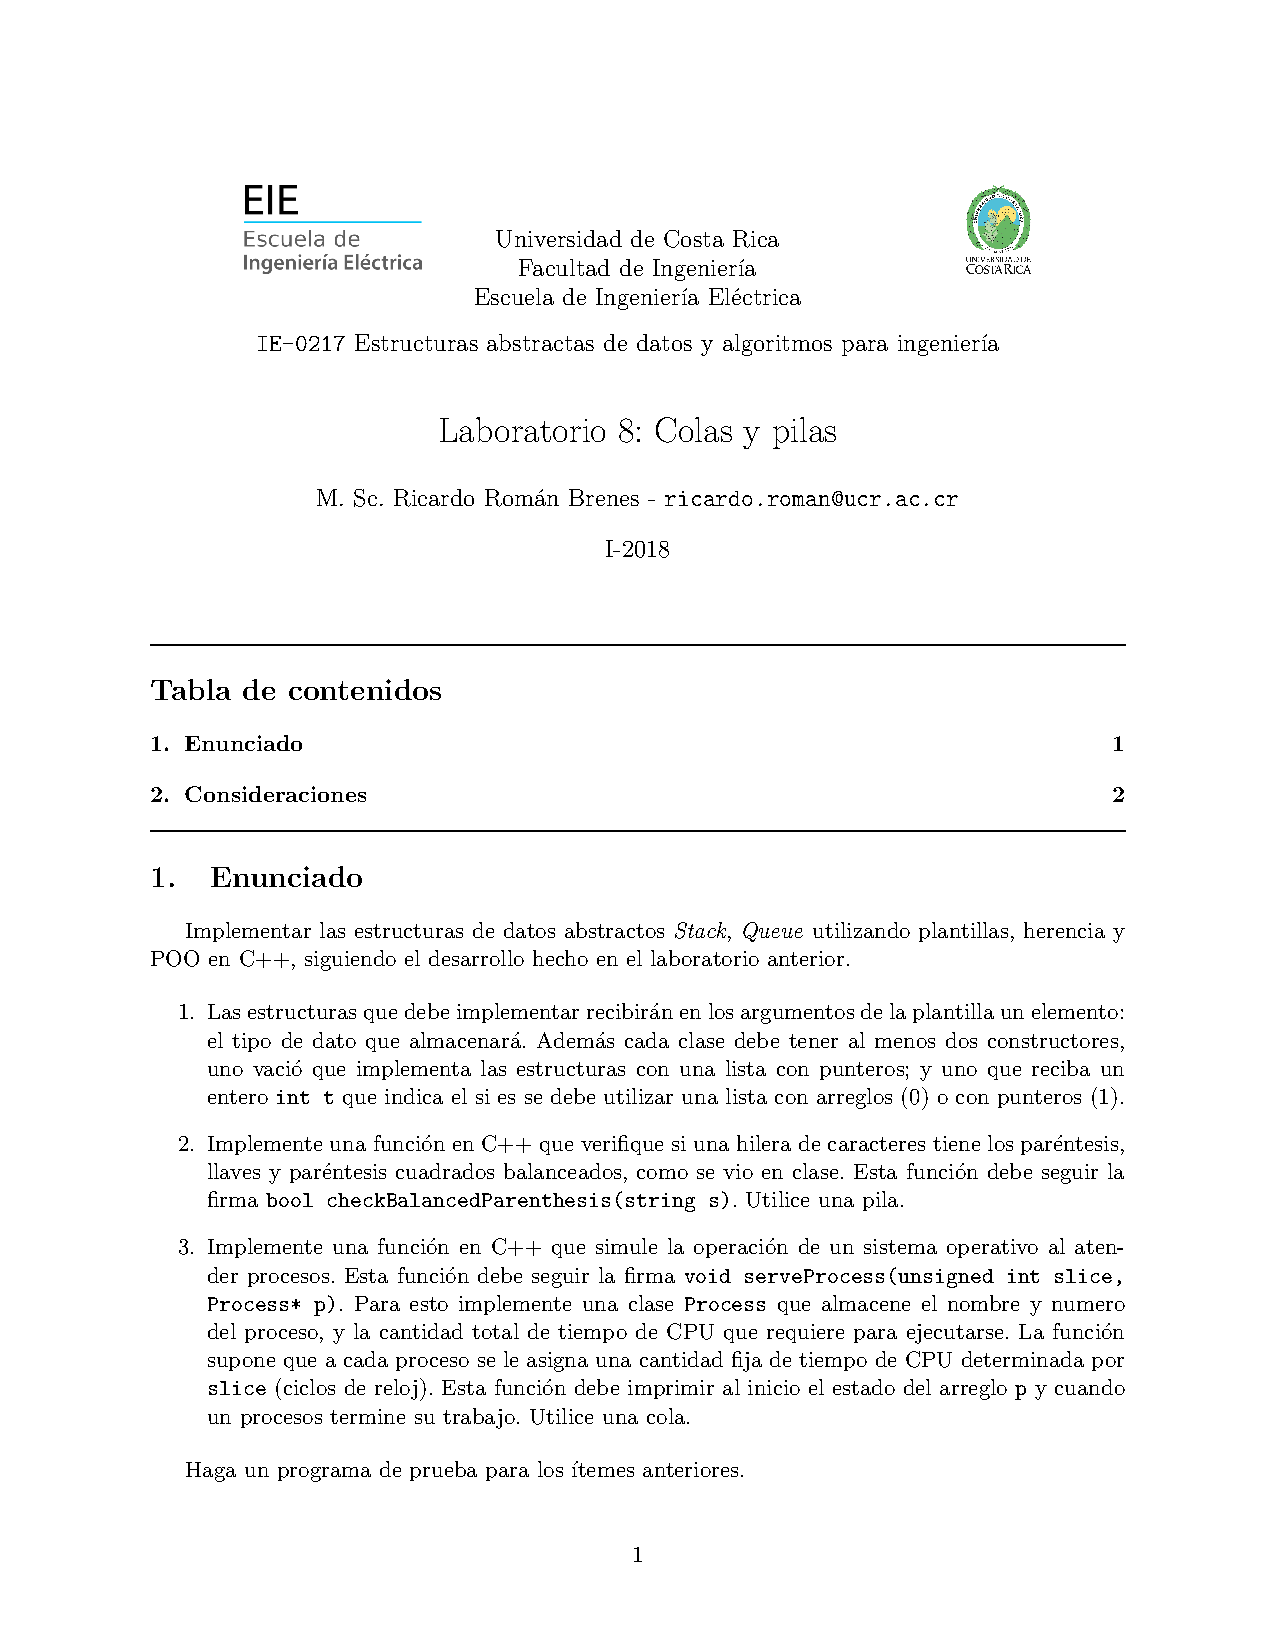
\includepdf[pages=1,pagecommand=\section{Enunciado}, scale=0.8]{enunciados/enun8} 
\includepdf[pages=2,pagecommand={},scale=0.8]{enunciados/enun8}

%%%%%%%%%%%%%%%%%%%%%%%%%%%%%%%%%%%%%%%%%%%%%%%%%%%%%%%%%%%%%%
% --> SOLUCIÓN
%%%%%%%%%%%%%%%%%%%%%%%%%%%%%%%%%%%%%%%%%%%%%%%%%%%%%%%%%%%%%%
\section{Solución}

%--------------------------------------------------------------
\subsection{Cola}
%--------------------------------------------------------------
La cola es un caso especial de una lista con punteros, ya que tiene condiciones especiales que debe cumplir. Una cola tiene una estructura de tipo FIFO (first in first out) es decir, el primer elemento que entra a la estructura es el primer elemento en salir. Por lo tanto, para seguir estas restricciones, utilizando los métodos expuestos en la clase List.h, habrán algunos que no serán implementados pues no tienen sentido en una cola. Por lo tanto se proceden a implementar los siguientes:

\begin{figure}[H]
\centering
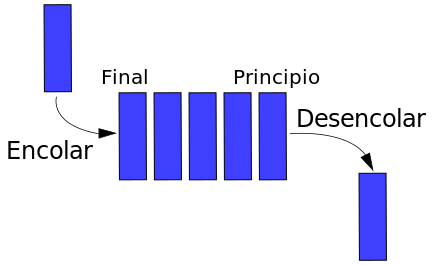
\includegraphics[width=0.35\textwidth]{imgs/Labo8/cola.png}
\caption{Estructura de datos tipo cola}
\label{fig:cola}
\end{figure}

%--------------------------------------------------------------
\subsection{Pila}
%--------------------------------------------------------------

La pila básicamente es una lista con punteros que tiene ciertas restricciones. Una pila es una estructura tipo LIFO (last in first out) de manera entonces que el último elemento que entra es el único que puede salir. Debido a esta restricción entonces limita un poco la implementación de todos los métodos definidos en la clase abstracta List.h que podemos observar en la sección 2.2. Tomando esto en cuenta nos damos que de los métodos virtuales puros solo podemos implementar los siguientes.

\begin{figure}[H]
\centering
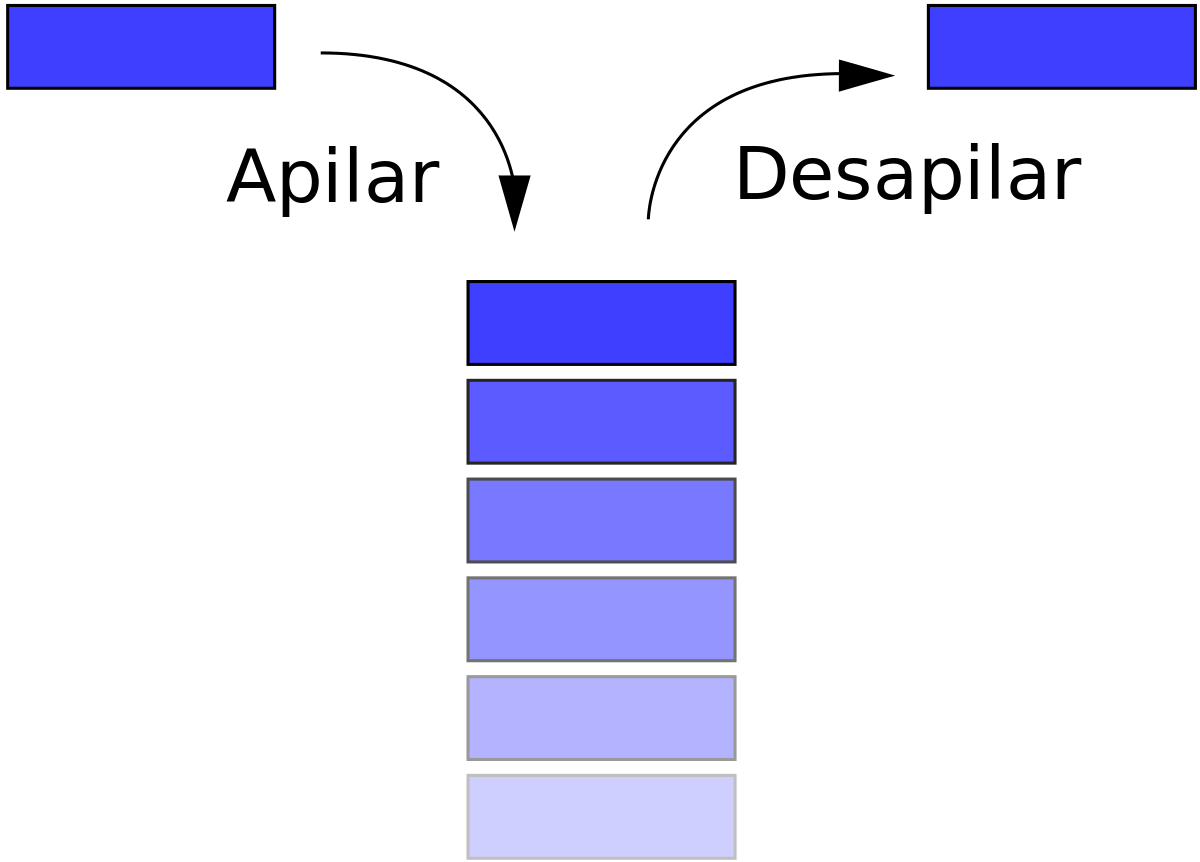
\includegraphics[width=0.35\textwidth]{imgs/Labo8/pila.png}
\caption{Estructura de datos tipo pila}
\label{fig:pila}
\end{figure}



\begin{minted}[linenos,autogobble,bgcolor=bg,breaklines,fontsize=\footnotesize ]{c++}
#include <string>
#include <iostream>
using namespace std;

class FileUtil
{
  public:
  	FileUtil(string s, ios_base::openmode p);
  	~FileUtil();
  	string read();
  	string* readLines();
  	int write(string s);
  	int write(string* s, int n);
    void countNumberLines();
    int getNumberLines();
  private:
    //Numero de lineas.
    int numLines;
    //Dirección de lectura.
    string ruta;
    //Modo de lectura.
  	ios_base::openmode modo;
    //Linea leida.
    string line;
    //Puntero con la direccion del arreglo de las lineas leidas.
    string* lines;

};
\end{minted}



%%%%%%%%%%%%%%%%%%%%%%%%%%%%%%%%%%%%%%%%%%%%%%%%%%%%%%%%%%%%%%
% --> RESULTADOS
%%%%%%%%%%%%%%%%%%%%%%%%%%%%%%%%%%%%%%%%%%%%%%%%%%%%%%%%%%%%%%
\section{Resultados}



%%%%%%%%%%%%%%%%%%%%%%%%%%%%%%%%%%%%%%%%%%%%%%%%%%%%%%%%%%%%%%
% --> CONCLUSIONES
%%%%%%%%%%%%%%%%%%%%%%%%%%%%%%%%%%%%%%%%%%%%%%%%%%%%%%%%%%%%%%
\section{Conclusiones}


Como conclusiones se tiene que:

\begin{itemize}
\item 
\item 
\item 
\item 
\end{itemize}


%%%%%%%%%%%%%%%%%%%%%%%%%%%%%%%%%%%%%%%%%%%%%%%%%%%%%%%%%%%%%%
% --> BIBLIOGRAFIA
%%%%%%%%%%%%%%%%%%%%%%%%%%%%%%%%%%%%%%%%%%%%%%%%%%%%%%%%%%%%%%
\begin{thebibliography}{IEEE}
\bibitem{R1} Talens, S. \textbf{\textit{Curso de programación en C++}}. EUI (UPV) Valencia, 17 al 28 de Julio de 1995. 

\bibitem{R2} Raffo, E. \textbf{\textit{Programación genérica en C++, usando Metaprogramación}}. 2007. Sistemas de Informática. 

\bibitem{R3} Quevedo, E.; López, R. \& Asencio, A. \textbf{\textit{Programación. Tema 4: Pilas y Colas}}. 2014. Sistemas de Informática. 

\end{thebibliography}

%%%%%%%%%%%%%%%%%%
%--> PROYECTO 1
%%%%%%%%%%%%%%%%%%
%\input{tex/proy1.tex}

\end{document}